\documentclass[a4paper,twoside,11pt]{article}
\usepackage[ngerman]{babel}
\usepackage[T1]{fontenc}
\usepackage[left=2cm,right=3cm]{geometry}
\usepackage{graphicx}
\usepackage{pdfpages}
\usepackage{tabto}
\usepackage{setspace}
\begin{document}

\begin{center}
\begin{huge}
	\par\bigskip
	\par\bigskip
	\par\bigskip
	\par\bigskip	
	\par\bigskip
	\par\bigskip	
	\textbf{Projektarbeit}\\
	\par\bigskip
	\par\bigskip	
	\par\bigskip
	\par\bigskip	
	\textbf{Auslegung eines alternativen Modellflügels für das Flugzeug „Zaunkönig“} \\
	\textbf{in Glasfaserverbund-Holm-Bauweise}\\
	\par\bigskip
	\par\bigskip
	
	\end{huge}

	\par\bigskip
\par\bigskip	
\par\bigskip
\par\bigskip
	\par\bigskip
\par\bigskip	
\par\bigskip
\par\bigskip	
	\par\bigskip
\par\bigskip	
\par\bigskip
\par\bigskip	
	Hannes Golombek, einfügen\\
	Ole Scholz, einfügen \\
	Henri Kammler, 4947286\\
	Tristan Brack, 4968977\\
\par\bigskip
\par\bigskip	
\par\bigskip

Betreut von Malte Woidt\\
\par\bigskip
\par\bigskip	
\par\bigskip
\par\bigskip	
\par\bigskip
\par\bigskip	
21.01.2021\\
\end{center}


\newpage
Test Aufgabenstellung
\newpage
\input{Projektarbeit - Übersicht}
\newpage
\tableofcontents
\newpage
\section{Bezeichnungen}
\textbf{Bezeichnungen}
\begin{table}[h]

\begin{tabular}{ll}
	$ A $&Festlager, (hoch gestellt) in Bezug auf Wirkebene, (mit 0 als Index) umschlossene Fläche\\
	$ B $&Loslager\\
	$ C $&Krafteinleitung der Querkraftbolzen\\
	$ E $&Elastizitätsmodul (allgemein)\\
	$ F $&Kraft (allgemein)\\
	FKV&Faser-Kunststoff-Verbund\\
	$ G $&Schubmodul (allgemein)\\
	GFK& Glasfaser-Kunstoffverbund\\
	$ I $&Flächenträgheitsmoment (allgemein)\\
	$ K $&Dimensionierungskennwert nach [QUELLE VDI einfügen], (zweifach unterstrichen) Elementsteifigkeistmatrix\\
	$ Q $&Querkraft (allgemein)\\
	$ R $&Integrationskonstante (allgemein), Festigkeit\\
	$ P $&Gewichtsnormalisierte Festigkeit\\
	$ S $&Statisches Moment\\
	$ T $&Bei Torsion\\
	UD&unidirektional\\
	Fb&Faserbruch\\
	Zfb&Zwischenfaserbruch\\
	
\end{tabular}
\end{table}

\begin{table}[h]
	\begin{tabular}{ll}
		$ a $&Lange Seite des Streifens nach \cite{item1}\\
		$ b $&Kurze Seite des Streifens nach \cite{item1}, bei Biegung\\
		$ f $&(mit E als Index) Anstrengung\\
		$ h $&Höhenabmessung des Holmes (allgemein)\\
		$ j $&Sicherheitsfaktor\\
		$ l $&Längenabmessung des Holmes (allgemein)\\
		$ n $&Lagenanzahl, Normalkraftfluss\\
		$ p $&Steigungs-/Neigungsparameter\\
		$ q $&Schubfluss\\
		$ \bar{q} $&Flächengewicht nach [Quelle VDI einfügen]\\
		$ s $&Dicke des Streifens nach \cite{item1}, Laufvariable in der	y-z-Ebene\\
		$ t $&Dicke des Verbunds nach \cite{item3}\\
		$ w $&Absenkung des Balkens unter Prüfkraft\\
		$ x $&x-Koordinate in Flugzeuglängsrichtung\\
		$ y $&y-Koordinate in Holmrichtung, positiv Richtung Endrippe\\
		$ z $&z-Koordinate der Rechtssystems\\
		
	\end{tabular}
\end{table}

\begin{table}[h]
	\begin{tabular}{ll}
		$ \epsilon $&Dehnung (allgemein)\\
		$ \eta $&Schwächungsfaktor\\
		$ \vartheta $&Verdrillung\\
		$ \theta $ &Winkel der Bruchebene\\
		$ \varphi $&Faservolumengehalt, Winkel zwischen Hauptachsen- und Schwerpunkt-Koordinatensystem\\
		$ \phi $&Orientierungsabweichung\\
		$ \kappa $&Steifigkeitserhöhung des Sandwich nach \cite{item1}\\
		$ \rho $&Dichte (allgemein)\\
		$ \sigma $&Zug-/Druckspannung (allgemein)\\
		$ \tau $&Schubspannung (allgemein)\\
	\end{tabular}
\end{table}

\begin{table}[h]
	\begin{tabular}{ll}
		$ 11 $&Faserhauptrichtung\\
		$ 22 $&Fasernebenrichtung\\
		$ 12 $&Wie heißt diese Richtung ?????\\
		$ \parallel $&Parallel zur Faser\\
		$ \perp $&Senkrecht zur Faser\\
		$ \# $&Unter 45° zur Faserrichtung\\
		$ + $&Bei Zugbeanspruchung\\
		$ - $&Bei Druckbeanspruchung\\
		$ \bar{ } $&Bei Schwerpunkt-Koordinaten\\
		$ \hat{ } $&Bei Hauptachsen-Koordinaten\\
		$ I $ &Holmbereich zwischen A und B\\
		$ II $ &Holmbereich zwischen B und C\\
		$ III $ &Holmbereich von C bis Flügelspitze\\
		1 bis 10? & Bereiche Schubmittelpunktberechnung????
	\end{tabular}
\end{table}


\newpage
\section{Einleitung}
\subsection{Projektbeschreibung}
Der Zaunkönig ist ein in den frühen 1940er Jahren entstandenes Flugzeug, das unter der Leitung von Hermann Winter an der TU-Braunschweig konstruiert wurde. (Quelle: Wikipedia (bessere Quelle suchen)) Da der Zaunkönig damals vornehmlich aus Holz gebaut wurde soll jetzt ein neuer Flügel im Maßstab 1:4,7 aus Glasfaser Kunststoffverbund (GFK) konstruiert werden. Der Flügel muss gewisse Anforderungen erfüllen, die im nachfolgenden definiert werden.
Bei dem Flügel handelt es sich um einen Rechteckflügel und ist an den Punkten l=1/4 l und l=1/2 l über Verstrebungen mit dem Rumpf verbunden. Diese Streben sollen in der neuen Konstruktion nicht vorhanden sein. Der Flügel soll im Rumpf verstiftet werden, wobei die Torsionsbelastung durch Querkraftbolzen aufgenommen wird. Insgesamt darf der Flügel das Gewicht von 0,750 kg nicht überschreiten.
Um die strukturmechanischen Anforderungen zu erfüllen wird der Flügel auf seine Steifigkeit und Festigkeit geprüft. Die Steifigkeit ist hinreichen, wenn der Flügel bei einer senkrechten Belastung von 100 N am L/4- Punkt, eine Durchbiegung von z=22mm nicht überschreitet. Außerdem darf der Flügel bei einer Prüfkraft von 500 N nicht brechen. Die Haut muss so ausgelegt sein, dass kein Beulen auftritt. Zusätzlich müssen der Torsionswinkel und Torsionsmittelpunkt berechnet werden.
\subsection{Motivation}
Zunächst ist zu klären, warum es überhaupt sinnvoll ist für diesen Flügel GFK zu verwenden. In der Luftfahrt wird immer nach Wegen gesucht das Gewicht zu minimieren, um die Wirtschaftlichkeit von Flugobjekten zu maximieren. Faser-Kunststoffverbunde (FKV) mit ihrer hohen spezifischen Festigkeit stellen hierbei einen idealen Kandidaten dar. Zusätzlich bieten FKV einfache Formgebung für komplexe aerodynamische Profile und auch die Korrosionsbeständigkeit ist höher, als bei konventionellen Werkstoffen. Als ein großer Nachteil ist hier jedoch der hohe Preis zu nennen, der jedoch in unserem Fall keine große Rolle spielt, da wir nur ein Modell entwerfen und der Flügel nicht für hohe Stückzahlen konstruiert wird. Glasfasern sind im Vergleich zu Kohlenstofffasern die günstigere Variante, aber auf Glasfasern wird in Kapitel 2.1 noch mal genauer eingegangen.
\subsection{Herangehensweise}
Im ersten Kapitel werden zunächst verschieden Lösungsvarianten und allgemeine Informationen zum Thema GFK Materialien vorgestellt. Daraufhin wird eine Lösungsvariante festgelegt. Um die Anforderungen zu erfüllen werden in Kapitel 3 Handbuchmethoden verwendet um eine Grobauslegung des Flügels durchzuführen. In Kapitel 4 werden diese dann mit Hilfe der Finiten Elemente Methode verifiziert. In Kapitel 5 werden die Ergebnisse mit den Konstruktionen vorheriger studentischer Arbeiten verglichen.
\newpage
\section{Grundlagen}
\subsection{Glasfaser}
Glasfasern gelten als älteste synthetische Faserart und wurden schon vor 3500 Jahren verwendet. Heute werden Glasfasern überwiegend aus SiO2 und Metalloxiden hergestellt. Die Bestandteile werden bei ca. 1400°C aufgeschmolzen und durch kleine Düsen im Boden des Kessels als dünne Fäden ausgelassen. Die Fäden werden aufgewickelt und zu größeren Fasern versponnen (vgl. \cite{item3})
Die hohe Festigkeit der Glasfaser beruht auf den kovalenten Bindungen von Silizium- und Sauerstoff-Atomen. Zugesetzte Metalloxide verhindern eine Ausbildung eines geordneten Gefüges und erhöhen somit zusätzlich die Festigkeit. Die Fasern können in Längsrichtung sehr hohe Kräfte aufnehmen, jedoch nicht in Querrichtung. Deshalb werden sie in eine Matrix integriert, die die Querkräfte aufnimmt und die Faser vor dem Knicken schützt. Glasfasern lassen sich auch um enge Radien sehr gut drapieren und sind durch ihre einfache Herstellungsweise sehr preiswert [4].
Durch die zuvor erläuterten Eigenschaften sind Glasfasern sehr gut für dieses Projekt geeignet, für einen größeren Flügel wäre jedoch der Elastizitätsmodul zu gering und es müsste auf andere Fasern, wie zum Beispiel Kohlefasern zurückgegriffen werden. 
Für die Konstruktion des Flügels stehen die Glasfasern Interglas 90070 und Interglas 92145 des Herstellers Interglas Technologies zur Verfügung. 

\subsection{Matrix}
Unter der Matrix versteht man den die Fasern umgebenden Teil des Faserverbundstoffs. Dabei werden im Bereich des Faser-Kunststoff-Verbunds Polymere wie z.B. Epoxidharz verwendet. Die Matrix ist meist der schwache Teil des FKV und ist dafür da um die Fasern gegen Knicken bei Druckbelastung zu schützen und eine gleichmäßige Krafteinleitung in die Fasern zu ermöglichen. Zusätzlich hält sie die Fasern in Position und verhindert Reibung zwischen den einzelnen Fasern.\\ 
\subsection{Netztheorie}
Text folgt noch
\subsection{Klassische Laminattheorie}
Text folgt noch
\subsection{Versagenskriterium nach Puck}
Text folgt noch
\subsection{Bauweise}
In der Aufgabenstellung wird gefordert, dass der Flügel in der Holm-Bauweise konstruiert wird. Ein Holm besteht aus zwei parallelen Gurten, die durch einen oder mehrere Stege miteinander verbunden werden. Dabei sind verschiedene Varianten möglich. Abbildung ~\ref{fig: Holmarten} veranschaulicht Konstruktionsmöglichkeiten. Neben der Festigkeit ist die Steifigkeit die einzige strukturmechanische Anforderung. Somit lässt sich das Problem als Biegebalken betrachten, der bei der vorgegebenen Prüflast $ F_{pruef}=100N $ am freien Ende die vorgegebene Durchbiegung $ w(100N)=22mm $ einhält. Das entstehende Biegemoment wird hauptsächlich von den Gurten getragen, weswegen man sich bei der Wahl des Steges auf andere Kriterien konzentrieren kann. Da kein maximaler Drillwinkel vorgegeben ist und die Torsionssteifigkeit fast ausschließlich von der Haut bewirkt wird, führen mehrere Stege, wie man sie bei einem geschlossenen Profil hat, nur zu unerwünschter Gewichtszunahme. Nach diesen Überlegungen wurde der I-Holm ausgewählt, da dieser bei einfacher Fertigung die gewünschten Eigenschaften mit sich bringt.
\begin{figure}
	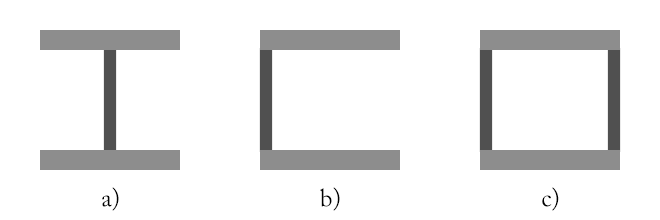
\includegraphics[width=1.0\textwidth]{Bilder/Holmarten.png}
	\caption{a) I-Holm   b) C-Holm    c) Kastenholm}
	\label{fig: Holmarten}
\end{figure} 
Das aerodynamische Profil des Flügels wird durch Schalenbauweise erreicht. Hierbei wir eine dünne Haut nur an kritischen Stellen mit der Sandwichbauweise beziehungsweise Rippen an den kritischen Stellen verstärkt, um Beulen zu verhindern. Die Schale trägt dabei so gut wie gar nicht die Last des Flügels, jedoch ist sie für die Torsionssteifigkeit entscheidend.

\newpage
\section{Modellierung des Holms}
\subsubsection{Einführung in die Balkenbiegung (T.B.)}
Anhand der \textit{Balkentheorie nach Bernoulli} soll im Folgenden das mechanische Verhalten des Holms unter gegebenen Bedingungen ermittelt werden. Dazu werden einführend diese Theorie und andere Zusammenhänge kurz dargestellt.\\

\noindent Die Balkentheorie beschreibt elastische Längs- und Querverformungen eines Balkens beliebigen Querschnitts, resultierend durch angreifende Kräfte, Streckenlasten und Momente. Diese können durch Lager oder äußere angreifende Lasten in einen solchen Körper eingeleitet werden. Ergänzend sei angemerkt, dass es sich bei einem Balken um einen Körper handelt, dessen Länge sehr viel größere Werte als die der Breite und der Höhe besitzt. Durch die Lasten herrschen im Balken innere Normal- und Querkräfte und innere Momente $(N, Q, M)$. Mittels des Freischneidens können diese an beliebigen Stellen berechnet werden. Folgend ergeben sich Normal- (Zug, Druck) und Schubspannungen $(\sigma, \tau)$, die wiederum über das \textit{Hooke´sche Gesetz} zu Dehnungen und Verzerrungen $(\epsilon, \gamma)$ führen, sodass letztendlich anhand derer beschriebene Verformungen $(u, v, w)$ zu erkennen sind. Durch das hohe Verhältnis der Abmessungen zueinander werden Schubspannungen im Weiteren vernachlässigt. \\

\noindent Für die Reaktionseigenschaften auf angreifende Lasten sind Materialkennwerte und die Geometrie des Balkens verantwortlich, welche mit der Biegesteifigkeit $EI$ repräsentiert werden. Gebildet wird sie durch den E-Modul $E$ und das Flächenträgheitsmoment $I$. Während ersteres eine wichtige Eigenschaft eines Materials ist, ist letzteres von der Querschnittsform abhängig. Neben der eigentlichen Form können ebenfalls Steiner-Anteile das Flächenträgheitsmoment erhöhen. Für die zu verwendenden Formeln wird auf das spätere Kapitel 5.1.3 verwiesen.\\


\noindent Innerhalb des gebogenen Balkens gibt es stets eine neutrale Faser, die eine Linie bzw. Fläche ohne eine relative Längenänderung unter angreifenden Kräften und Momenten repräsentiert. Diese Linie wird auch Biegelinie genannt, für welche die vereinfachte \textit{Differentialgleichung des Biegebalkens}
\begin{equation}
	w^{''}=-\frac{M}{EI}
\end{equation}
aufgestellt wurde. Neben der Krümmung $w^{''}$ kann mittels Integration der Biegewinkel $w^{'}$ und die Absenkung $w$ bestimmt werden. Über Differentiationen werden auch äußere Momente, Kräfte und Streckenlasten in der Balkentheorie mit einbezogen. Durch Integrationskonstanten können geometrische Rand- und Übergangsbedingungen beachtet werden. Während in der neutralen Faser keine Normalspannungen auftreten, sind diese in den Randfasern maximal.\\

\noindent Es sei außerdem angemerkt, dass jederzeit Superpositions-Eigenschaften gelten. Dadurch können einerseits mehrere Balken in einem System betrachtet werden, andererseits aber auch Balken mit mehreren Belastungen in einzelne einfache Berechnungen überführt werden.\\

\noindent Für die Berechnung einer Balkenbiegung kann nach folgendem Schema vorgegangen werden: Vorerst werden die notwendigen Lagerkräfte und -momente bestimmt. Wichtige Lagerarten bilden dabei das Festlager (ein rotatorischer Freiheitsgrad), das Loslager (ein rotatorischer und ein translatorischer Freiheitsgrad) und eine Einspannung (keine Freiheitsgrade), die Freiheitsgrade seien dabei auf den zweidimensionalen Fall bezogen. Anschließend wird der Balken bereichsweise an  Unstetigkeiten (z.B. Lager oder Krafteinleitungspunkte und ändernde Geometrien) geschnitten, um innere Kräfte am entstandenen positiven und negativen Schnittufer zu ermitteln. Dadurch lassen sich in diesen markanten Orten relevante Rand- und Übergangsbedingungen der Differentialgleichung des Biegebalkens bestimmen. Abschließend führen Integrationen und Differentiationen dieser Gleichung und deren Lösung  zur Absenkung, dem Biegewinkel, der Krümmung sowie innerem Kraft- bzw. Momentverlauf.


\subsubsection{Annahmen zur Modellierung (T.B.)}
Das Koordinatensystem des Flügels entspricht einem allgemeinen Flugzeug-Koordinatensystem, sodass die Flügellängskoordinate durch $y$ definiert ist. Der Koordinatenursprung ist im Lager A positioniert, da es keinen allgemeinen Flugzeugschwerpunkt gibt. \\

\noindent Der Holm inklusive des Holmstummels wird für die Belastung durch eine Prüfkraft $F_{pruef}$ in negative z-Richtung als Biegebalken ausgelegt. Dafür ist er an zwei Stellen gelagert, am Lager $A$ und am Lager $B$. Die Lager entsprechen den Verstiftungen (siehe Bauteil U-Profil). Um eine Überbestimmung des Systems zu vermeiden, wird das Lager $B$ als Loslager angenommen. Die Querkraftbolzen werden nicht durch ein Lager, sondern durch eine zusätzlich angreifende Kraft $F_{Q}$ simuliert, da eine biegeweiche Wurzelrippe eine nicht definierbare, unbekannte Absenkung erlaubt.\\

\noindent Als Randbedingungen der Modellierung sind die Halbspannweite $s$ und die Absenkung $w$ (bezogen auf KOS) gegeben. Für die Absenkung $w$ soll eine Sicherheit $j=1,1$ gesetzt werden. Zwischen Lager $A$ und $B$ wird die Länge $l_{1}$ angenommen, zwischen Lager $B$ und der Wurzelrippe $C$ die Länge $l_{2}$. Die verbleibende Länge bis zur Flügelspitze, an der die Prüfkraft $F_{pruef}$ wirkt, wird $l_{3}$ bezeichnet. Die Halbspannweite $s$ wird, beginnend in der Mitte der Verstiftungen, bis zur Flügelspitze gemessen. Ausgehend von dem Holmstummelende bis zum Lager $A$ wird $l_{0}$ als Länge definiert. Diese Länge ist jedoch unerheblich für die Modellierung, sie wird erst für die Massenbestimmung benötigt.\\

\noindent Anhand der Randbedingungen und der Einspannvorrichtung für den Versuchsaufbau ergeben sich folgende Längen (ebenfalls in Abb. ~\ref{fig:Holmmodellierung}~ dargestellt): 
\begin{equation}
	s = 0,848 m
\end{equation}
\begin{equation}
	l_{0} = 0,03 m
\end{equation}
\begin{equation}
	l_{1} = 0,076 m
\end{equation}
\begin{equation}
	l_{2} = 0,037 m 
\end{equation}
\begin{equation}
	l_{3} = s - \frac{l_{1}}{2} - l_{2} = 0,773 m
\end{equation}
\begin{equation}
	w_{j=1,1} = \frac{1}{j} * w = \frac{1}{1,1} * 0,022 m = 0,02 m
\end{equation}
\begin{figure}
	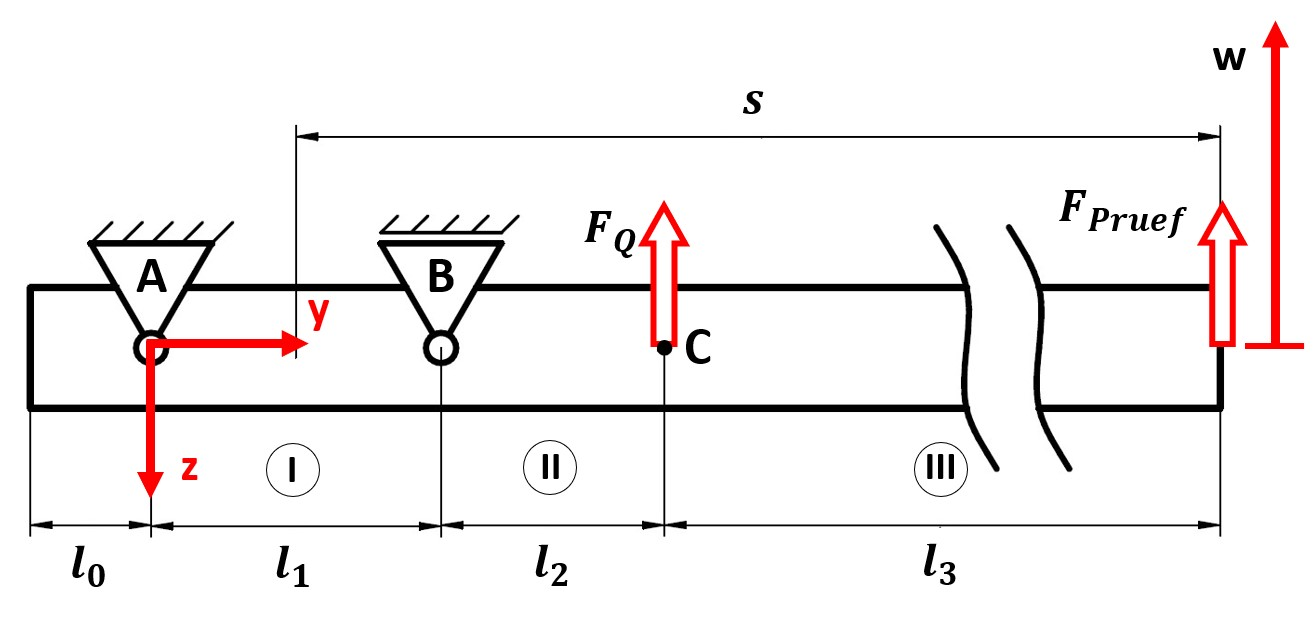
\includegraphics[width=1.0\textwidth]{Bilder/Balkenmodell2.jpg}
	\caption{Modellierung des Holms}
	\label{fig:Holmmodellierung}
\end{figure}

\subsubsection{Analytische Lösung der Modellierung (T.B.)}
Um die Differentialgleichungen der Balkenbiegung lösen zu können, wird der Biegebalken vorerst in drei Teilbereiche $I$, $II$ und $III$ aufgeteilt, die sich von Lager $A$ zu $B$, von Lager $B$ zur Wurzelrippe $C$ und von dort aus bis zur Flügelspitze erstrecken. \\

\noindent Dadurch ergeben sich folgende zwölf Differentialgleichungen:
\begin{equation} \label{eq:7}
	EI_{x}\cdot w_{I}^{''''}(y) = q_{I}(y)
\end{equation}
\begin{equation}\label{eq:8}
	EI_{x}\cdot w_{I}^{'''}(y) = q_{I}(y)\cdot y + R_{1} = -Q_{I}(y)
\end{equation}
\begin{equation}\label{eq:9}
	EI_{x}\cdot w_{I}^{''}(y) = \frac{q_{I}(y)}{2}\cdot y^{2} + R_{1}\cdot y + R_{2} = -M_{I}(y)
\end{equation}
\begin{equation}\label{eq:10}
	EI_{x}\cdot w_{I}^{'}(y) = \frac{q_{I}(y)}{6}\cdot y^{3} + \frac{R_{1}}{2}\cdot y^{2} + R_{2}\cdot y + R_{3} 
\end{equation}
\begin{equation}\label{eq:11}
	EI_{x}\cdot w_{I}(y) = \frac{q_{I}(y)}{24}\cdot y^{4} + \frac{R_{1}}{6}\cdot y^{3} + \frac{R_{2}}{2}\cdot y^{2} + R_{3}\cdot y + R_{4}
\end{equation}\\
\begin{equation}\label{eq:12}
	EI_{x}\cdot w_{II}^{''''}(y) = q_{II}(y)
\end{equation}
\begin{equation}\label{eq:13}
	EI_{x}\cdot w_{II}^{'''}(y) = q_{II}(y)\cdot y + R_{5} = -Q_{II}(y)
\end{equation}
\begin{equation}\label{eq:14}
	EI_{x}\cdot w_{II}^{''}(y) = \frac{q_{II}(y)}{2}\cdot y^{2} + R_{5}\cdot y + R_{6} = -M_{II}(y)
\end{equation}
\begin{equation}\label{eq:15}
	EI_{x}\cdot w_{II}^{'}(y) = \frac{q_{II}(y)}{6}\cdot y^{3} + \frac{R_{5}}{2}\cdot y^{2} + R_{6}\cdot y + R_{7} 
\end{equation}
\begin{equation}\label{eq:16}
	EI_{x}\cdot w_{II}(y) = \frac{q_{II}(y)}{24}\cdot y^{4} + \frac{R_{5}}{6}\cdot y^{3} + \frac{R_{6}}{2}\cdot y^{2} + R_{7}\cdot y + R_{8}
\end{equation}\\
\begin{equation}\label{eq:17}
	EI_{x}\cdot w_{III}^{''''}(y) = q_{III}(y)
\end{equation}
\begin{equation}\label{eq:18}
	EI_{x}\cdot w_{III}^{'''}(y) = q_{III}(y)\cdot y + R_{9} = -Q_{I}(y)
\end{equation}
\begin{equation}\label{eq:19}
	EI_{x}\cdot w_{III}^{''}(y) = \frac{q_{III}(y)}{2}\cdot y^{2} + R_{9}\cdot y + R_{10} = -M_{I}(y)
\end{equation}
\begin{equation}\label{eq:20}
	EI_{x}\cdot w_{III}^{'}(y) = \frac{q_{III}(y)}{6}\cdot y^{3} + \frac{R_{9}}{2}\cdot y^{2} + R_{10}\cdot y + R_{11} 
\end{equation}
\begin{equation}\label{eq:21}
	EI_{x}\cdot w_{III}(y) = \frac{q_{III}(y)}{24}\cdot y^{4} + \frac{R_{9}}{6}\cdot y^{3} + \frac{R_{10}}{2}\cdot y^{2} + R_{11}\cdot y + R_{12}
\end{equation}\\

\noindent Die Randbedingungen der Modellierung ergeben sich folgend nach gegebenen Definitionen von Lagern und angreifenden Kräften: 
\begin{equation}\label{eq:22}
	w_{I}(y=0)=0
\end{equation}
\begin{equation}\label{eq:23}
	M_{I}(y=0)=0
\end{equation}\\
\begin{equation}\label{eq:24}
	w_{I}(y=l_{1}) = 0
\end{equation}
\begin{equation}\label{eq:25}
	w_{II}(y=l_{1}) = 0
\end{equation}
\begin{equation}\label{eq:26}
	w_{I}^{'}(y=l_{1}) = w_{II}^{'}(y=l_{1})
\end{equation}
\begin{equation}\label{eq:27}
	M_{I}(y=l_{1}) = M_{II}(y=l_{1})
\end{equation}\\
\begin{equation}\label{eq:28}
	w_{II}(y=l_{1}+l_{2}) = w_{III}(y=l_{1}+l_{2})
\end{equation}
\begin{equation}\label{eq:29}
	w_{II}^{'}(y=l_{1}+l_{2}) = w_{III}^{'}(y=l_{1}+l_{2})
\end{equation}
\begin{equation}\label{eq:30}
	M_{II}(y=l_{1}+l_{2}) = M_{III}(y=l_{1}+l_{2})
\end{equation}
\begin{equation}\label{eq:31}
	Q_{II}(y=l_{1}+l_{2}) = Q_{III}(y=l_{1}+l_{2})+F_{Q}
\end{equation}\\
\begin{equation}\label{eq:32}
	M_{III}(y=l_{1}+l_{2}+l_{3})=0
\end{equation}
\begin{equation}\label{eq:33}
	Q_{III}(y=l_{1}+l_{2}+l_{3})=F_{pruef}
\end{equation}
Zusätzlich wird angenommen, dass $q_{I}(y)=q_{II}(y)=q_{III}(y)=0$ gilt, da keine Streckenlast angreift. Unter anderem bildet die Schwerkraft der Erde eine Streckenlast, diese kann jedoch aufgrund ihres kleinen Einflusses auf die Absenkung gegenüber der Prüfkraft vernachlässigt werden. Ein weiteres Beispiel für eine Streckenlast bildet die Auftriebsverteilung eines Flügels während einer Anströmung. Jedoch wird genau auf diese im Versuchsstand verzichtet und durch die Prüfkraft repräsentiert.\\

\noindent Als Lösung dieser Differentialgleichungen lässt sich die Querkraft $Q(y)$, das Moment $M(y)$ und die Biegelinie $w(y)$ ermitteln:\\

\begin{equation}\label{eq:34}
	Q(y,F_{pruef},F_{Q},EI_{x})=\left\{\begin{array}{ll}
		F_{pruef}\cdot \frac{l_{2}+l_{3}}{l_{1}}-F_{Q}\cdot \frac{l_{2}}{l_{1}}&,y\epsilon (0,l_{1})\\
		F_{pruef}+F_{Q}&,y\epsilon (l_{1}, l_{1}+l_{2})\\
		F_{pruef}&,y\epsilon (l_{1}+l_{2}, l_{1}+l_{2}+l_{3})
	\end{array}\right.
\end{equation}\\
\begin{equation}\label{eq:35}
	M(y,F_{pruef},F_{Q},EI_{x})=\left\{\begin{array}{ll}
		(-F_{pruef}\cdot \frac{l_{2}+l_{3}}{l_{1}}-F_{Q}\cdot \frac{l_{2}}{l_{1}})\cdot y&,y\epsilon (0,l_{1})\\
		F_{pruef}\cdot (y-l_{1}+l_{2}+l_{3})+F_{Q}\cdot (y-l_{1}+l_{2})&,y\epsilon (l_{1}, l_{1}+l_{2})\\
		F_{pruef}\cdot (y-l_{1}+l_{2}+l_{3})&,y\epsilon (l_{1}+l_{2}, l_{1}+l_{2}+l_{3})
	\end{array}\right.
\end{equation}\\
\begin{equation}\label{eq:36}
	w(y,F_{pruef},F_{Q},EI_{x})=\left\{\begin{array}{ll}
		\frac{1}{EI_{x}}\cdot\frac{1}{6}\cdot\biggl((F_{pruef}\cdot \frac{l_{2}+l_{3}}{l_{1}}-F_{Q}\cdot \frac{l_{2}}{l_{1}})\cdot y^{3}-\Bigl((l_{2}+l_{3})\cdot l_{1}\cdot F_{pruef}-l_{1}\cdot l_{2}\cdot F_{Q}\Bigl)\cdot y \biggr)&\\,y\epsilon (0,l_{1})\\
		\frac{1}{EI_{x}}\cdot\biggl(\frac{(-F_{pruef}-F_{Q})}{6}\cdot y^{3} + \frac{F_{pruef}\cdot (l_{1}+l_{2}+l_{3})+F_{Q}\cdot (l_{1}+L_{2})}{2}\cdot y^{2}\\ + \Bigl(F_{pruef}\cdot(-\frac{1}{2}\cdot l_{1}^{2}-\frac{2}{3}\cdot l_{1}\cdot l_{2}-\frac{2}{3}\cdot l_{1}\cdot l_{3})+ F_{Q}\cdot(-\frac{1}{2}l_{1}^{2}-\frac{2}{3}\cdot l_{1}\cdot l_{2})\Bigr)\cdot y \\+ F_{pruef}\cdot\frac{1}{6}\cdot(l_{1}^{3}+l_{1}^{2}\cdot l_{2}+l_{1}^{2}\cdot l_{3}) + F_{Q}\cdot\frac{1}{6}\cdot(l_{1}^{3}+l_{1}^{2}\cdot l_{2})\biggr)&\\,y\epsilon (l_{1}, l_{1}+l_{2})\\
		\frac{1}{EI_{x}}\cdot\biggl(-\frac{F_{pruef}}{6}\cdot y^{3} + \frac{ F_{pruef}\cdot (l_{1}+l_{2}+l_{3})}{2}\cdot y^{2} + \Bigl(F_{pruef} \\
		\cdot(-\frac{1}{2}\cdot l_{1}^{2} -\frac{2}{3}\cdot l_{1}\cdot l_{2}-\frac{2}{3}\cdot l_{1}\cdot l_{3}) + F_{Q}\cdot(\frac{1}{2}\cdot l_{2}^{2}+\frac{1}{2}\cdot l_{1}\cdot l_{2})\Bigr)\cdot y \\ +F_{pruef}\cdot\frac{1}{6}\cdot(l_{1}^{3}+l_{1}^{2}\cdot l_{2}+l_{1}^{2}\cdot l_{3}) + F_{Q}\cdot(-\frac{1}{6}\cdot l_{2}^{3}-\frac{1}{3}\cdot l_{1}^{2}\cdot l_{2}-\frac{1}{2}\cdot l_{2}^{2}\cdot l_{1})\biggr)&\\,y\epsilon (l_{1}+l_{2}, l_{1}+l_{2}+l_{3})
	\end{array}\right.
\end{equation}\\
Die Herleitung der Lösung kann im Kapitel \ref{Lösung} nachvollzogen werden.\\

\noindent Um nun für die später geforderte Biegesteifigkeit $EI_{x}$ ein Ergebnis zu erhalten, wird die Gleichung $w(y,F_{pruef},F_{Q}, EI_{x})$ nach $EI_{x}(y,F_{pruef},F_{Q},w)$ umgestellt. Die eingesetzten Werte ergeben sich aus der Auslegung auf Steifigkeit. Über die Wurzelrippe werden Kräfte des Holms in die Querkraftbolzen abgesetzt. Aufgrund der biegeweichen Wurzelrippe als Verbindungselement zwischen Holm und den Querkraftbolzen, darf die Absenkung des Holms dort nicht mit null angenommen werden. Vereinfacht wird definiert, dass die eingeleitete Prüfkraft $F_{pruef}$ an den Querkraftbolzen um ihren Betrag abgesetzt wird, wie es tatsächlich an einem Flugzeugrumpf geschehen würde. Dieses entspricht sehr wahrscheinlich jedoch nicht der tatsächlichen Kraftaufnahme im Versuchsaufbau.
\begin{equation}
	\begin{array}{l}
		EI_{x}(0.886m, 100N, -100N, 0.02m)= \\
		\frac{1}{w}\cdot\biggl(-\frac{F_{pruef}}{6}\cdot y^{3} + \frac{ F_{pruef}\cdot (l_{1}+l_{2}+l_{3})}{2}\cdot y^{2} + \Bigl(F_{pruef}\cdot(-\frac{1}{2}\cdot l_{1}^{2} -\frac{2}{3}\cdot l_{1}\cdot l_{2}-\frac{2}{3}\cdot l_{1}\cdot l_{3}) \\ +F_{Q}\cdot(\frac{1}{2}\cdot l_{2}^{2}+\frac{1}{2}\cdot l_{1}\cdot l_{2})\Bigr)\cdot y + F_{pruef}\cdot\frac{1}{6}\cdot(l_{1}^{3}+l_{1}^{2}\cdot l_{2}+l_{1}^{2}\cdot l_{3}) + F_{Q}\cdot(-\frac{1}{6}\cdot l_{2}^{3}-\frac{1}{3}\cdot l_{1}^{2}\cdot l_{2}-\frac{1}{2}\cdot l_{2}^{2}\cdot l_{1})\biggr)\\
		=962,552Nm^{2}
	\end{array}
\end{equation}

\subsubsection{Analyse der Modellierung (T.B.)}
In Abb. ~\ref{fig:Steifigkeitsauslegung} werden die Querkraftverläufe $Q(y,F_{pruef},F_{Q},EI_{x})$ als innere Schnittkraft, der Momentenverlauf $M(y,F_{pruef},F_{Q},EI_{x})$ als inneres Schnittmoment und die Biegelinie $w(y,F_{pruef},F_{Q},EI_{x})$ für den Nachweis der Steifigkeit graphisch dargestellt, über die gesamte Holmlänge und in einem vergrößerten Ausschnitt im Bereich der Lager. \\

\begin{figure}
	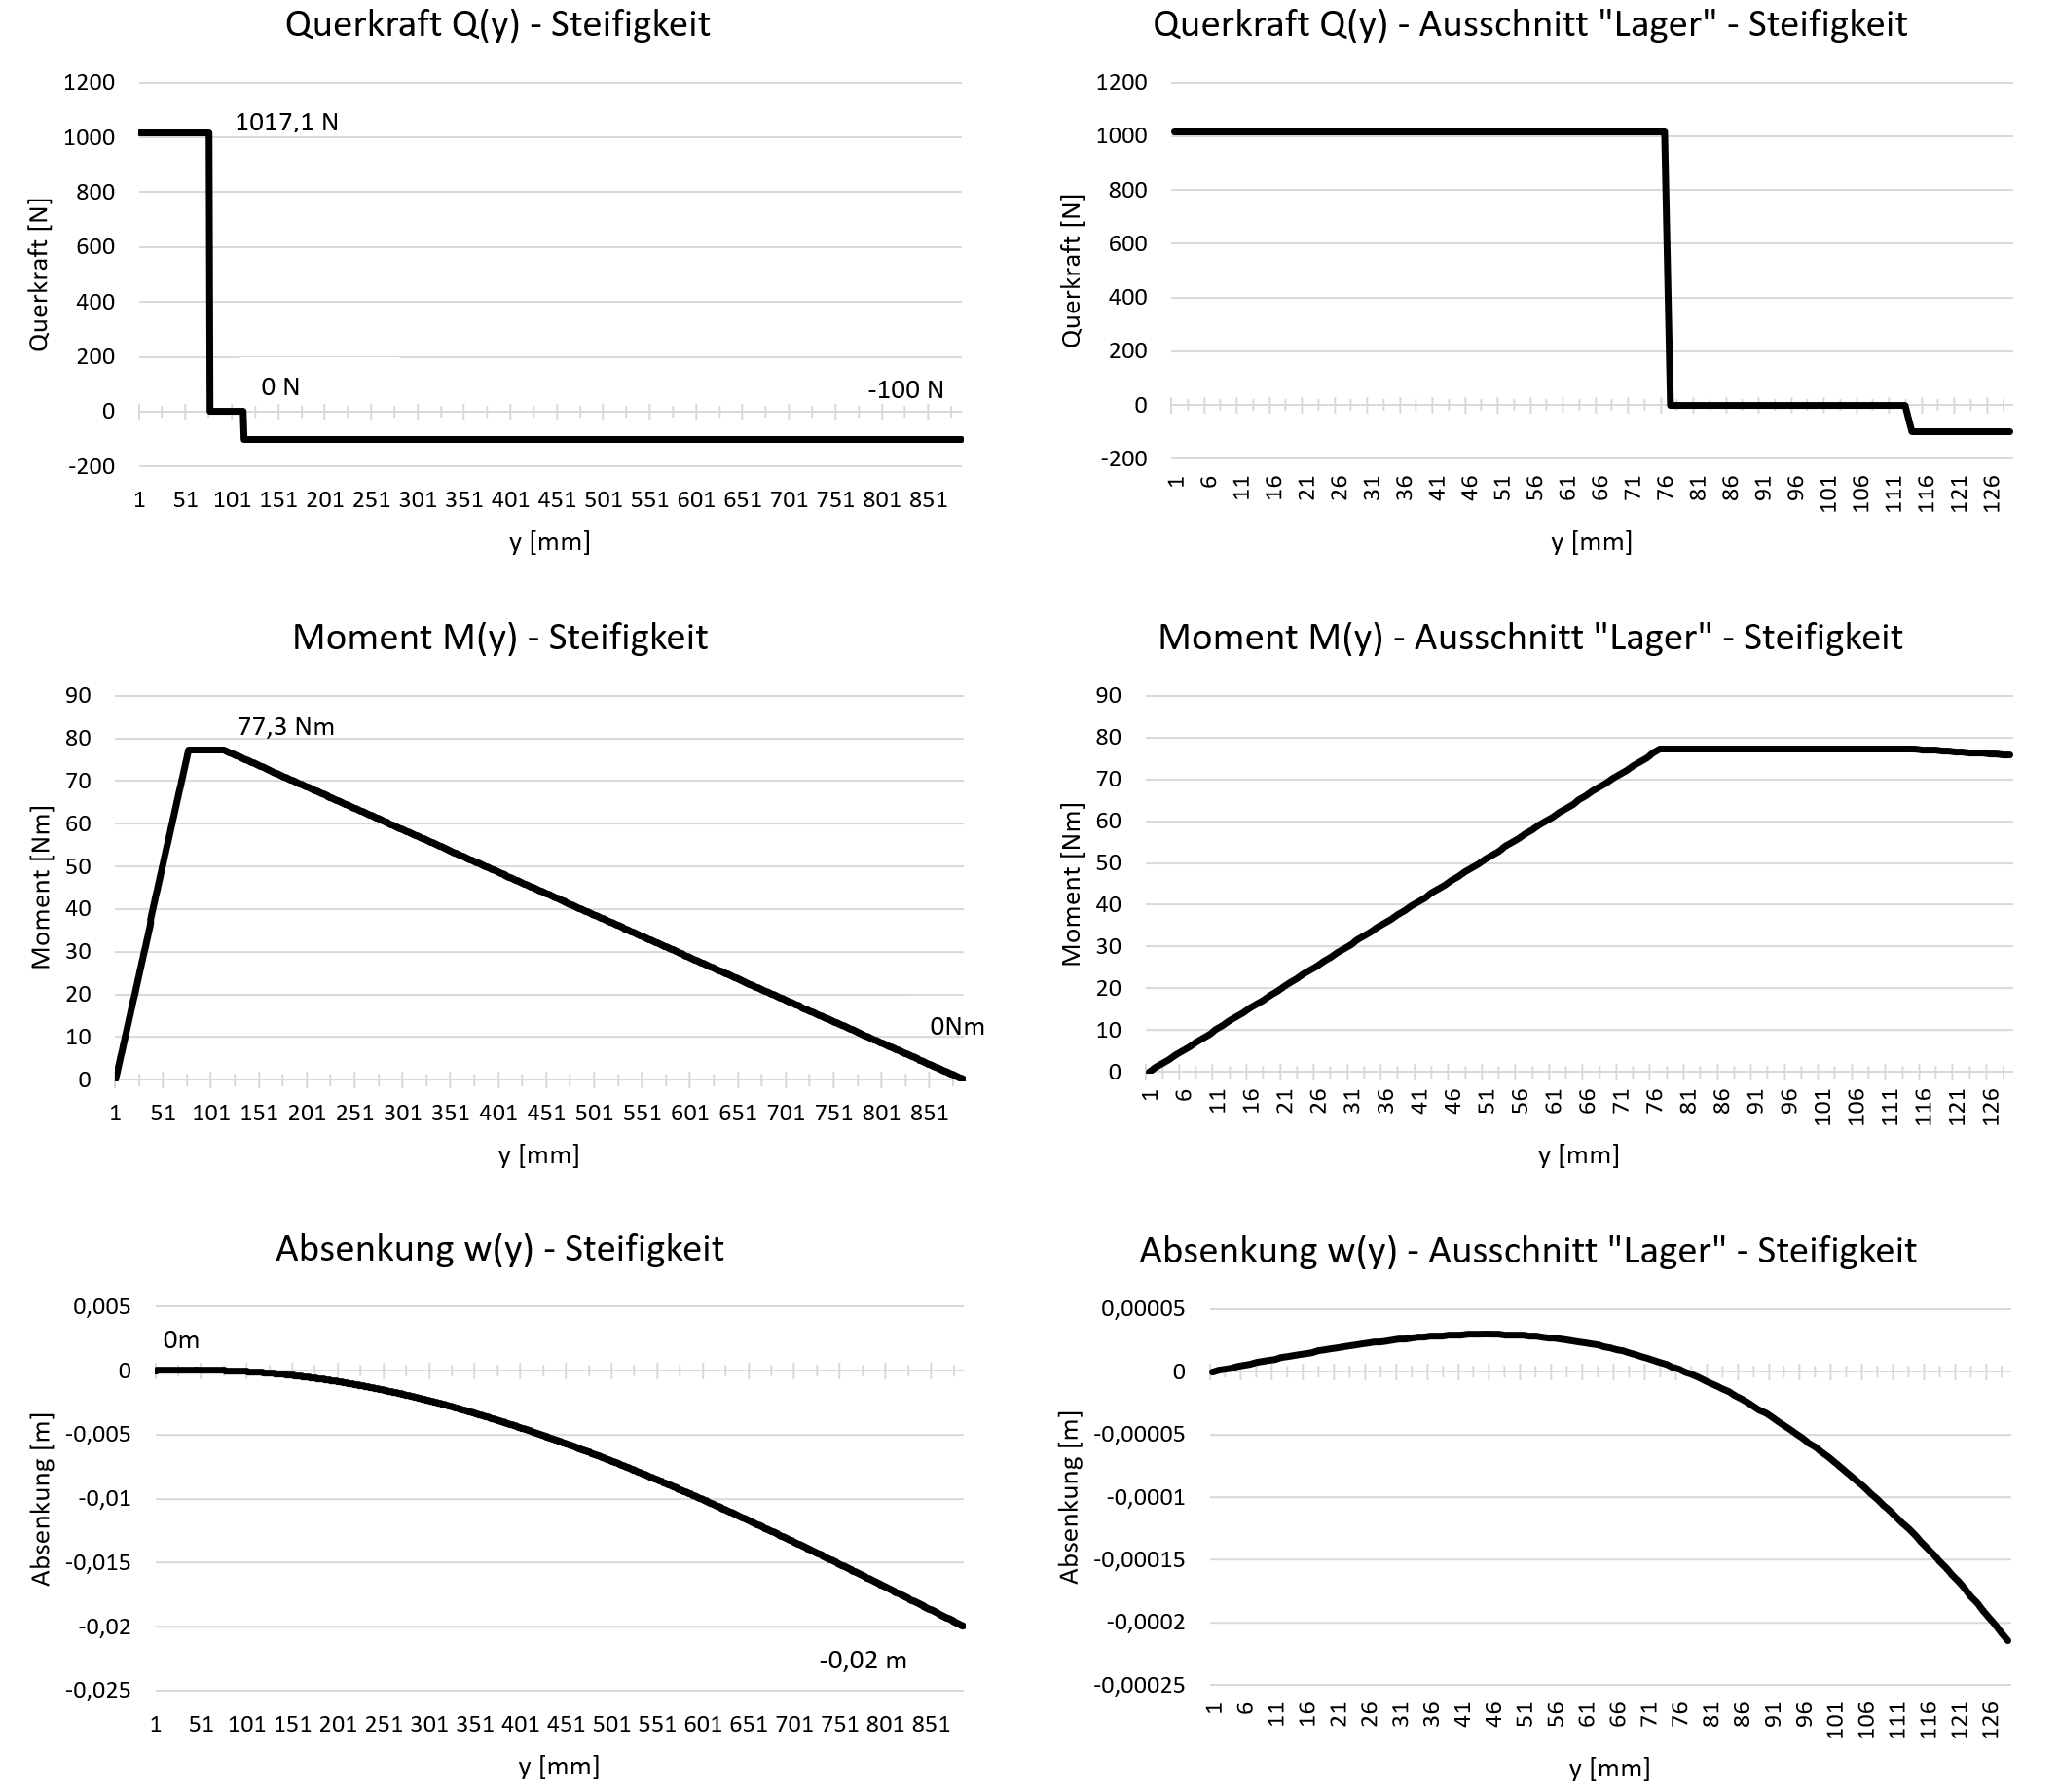
\includegraphics[width=1.0\textwidth]{Bilder/Grafiken Steifigkeit.png}
	\caption{Steifigkeitsauslegung}
	\label{fig:Steifigkeitsauslegung}
\end{figure}

\noindent Jedoch werden nicht bei dem Nachweis der Steifigkeit, sondern bei dem Nachweis der Festigkeit das maximale Schnittmoment und die maximale Schnittkraft erreicht. Bei diesem Nachweis beträgt die Prüfkraft $F_{pruef} = 500N$ und somit auch $|F_{Q}| = 500N$. Diese Kraft wird bei der Berechnung von $EI_{x}$ nicht beachtet, da bei dem Nachweis der Festigkeit die Absenkung $w$ kein Rolle spielt. In Abb. ~\ref{fig:Festigkeitsauslegung} werden die genannten Verläufe nun für den Festigkeitsnachweis dargestellt.
\begin{figure}
	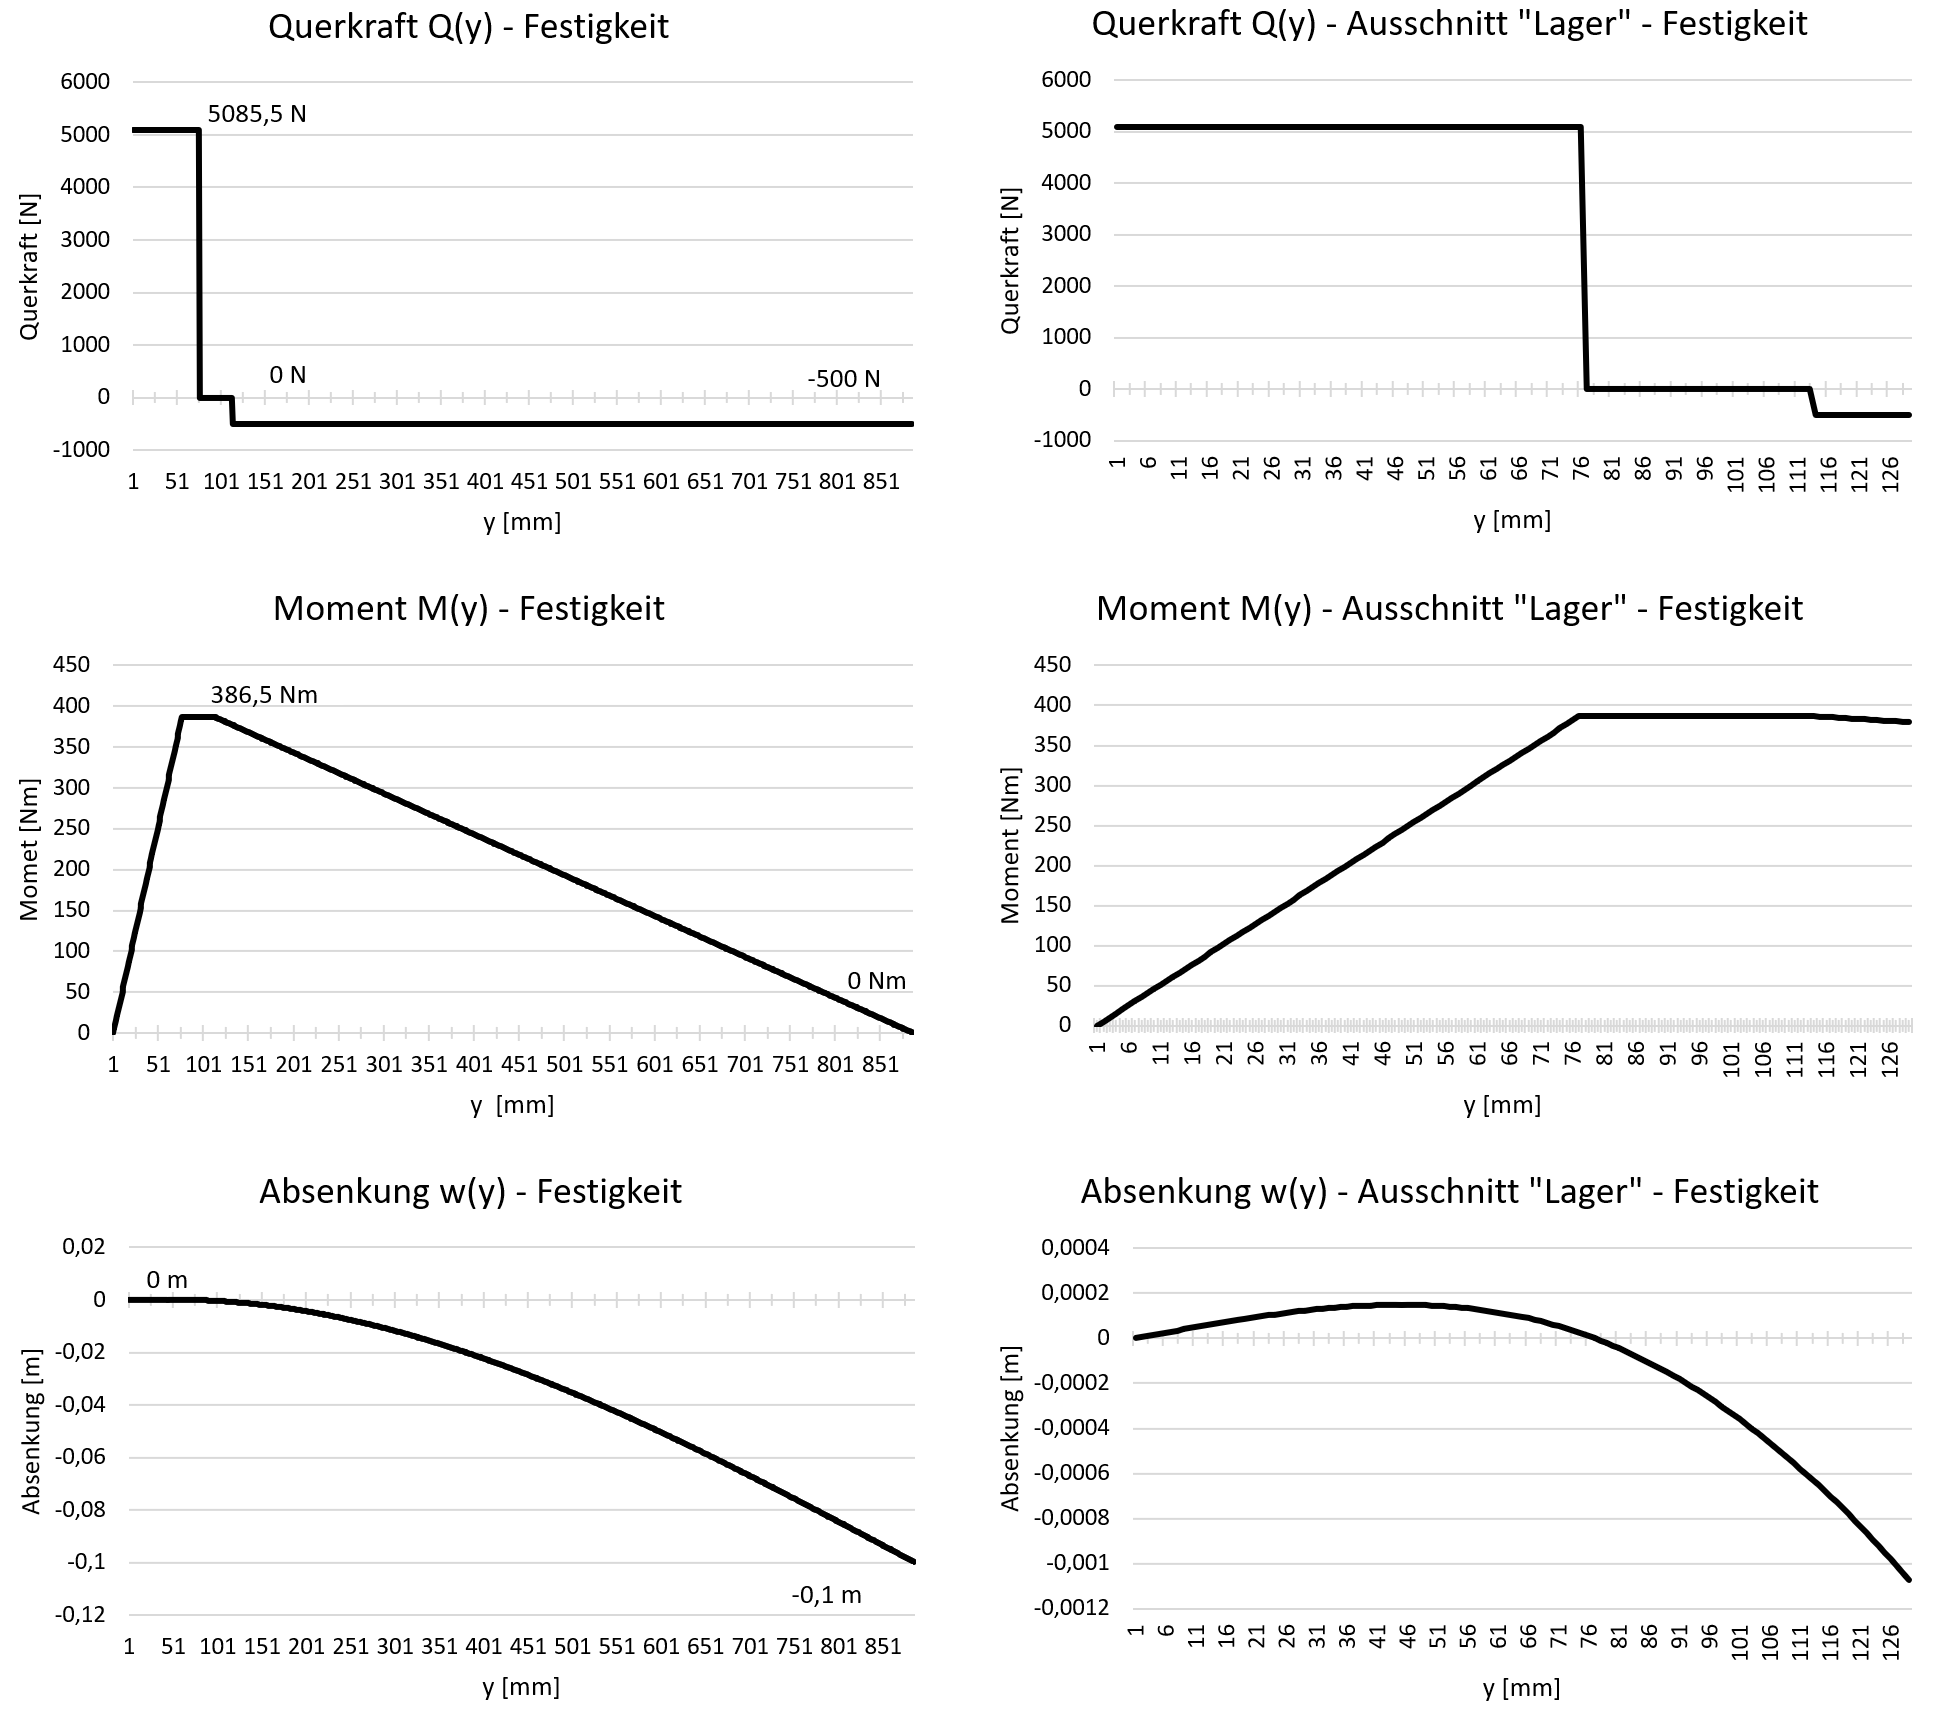
\includegraphics[width=1.0\textwidth]{Bilder/Grafiken Festigkeit.png}
	\caption{Festigkeitsauslegung}
	\label{fig:Festigkeitsauslegung}
\end{figure}


\newpage
\section{Auslegung des Holms nach VDI 2013 (H.K.)}
\label{VDI2013}

Auf Basis der in der Balkenberechnung bestimmten Parameter Biegesteifigkeit, maximales Biegemoment und der maximalen Querkraft, sollen die Gurte und der Steg dimensioniert werden. Die Vorauslegung soll dabei anhand der VDI- Richtlinie 2013 erfolgen, diese enthält in einem Unterkapitel Informationen speziell zur Auslegung eines I-Trägers. Dabei ist zu beachten, dass bei einigen Berechnungen Vereinfachungen angenommen werden, die an den betreffenden Stellen spezifiziert werden. Zusätzlich sei angemerkt, dass die erste Auslegung nur an an ausgewählten Stellen Sicherheitsfaktoren ungleich eins berücksichtigt. Grund dafür ist die Annahme, dass in den bereitgestellten Materialkennwerten ausreichende Sicherheiten verrechnet worden sind.

\subsection{Dimensionierung der Gurte}
\begin{figure}
	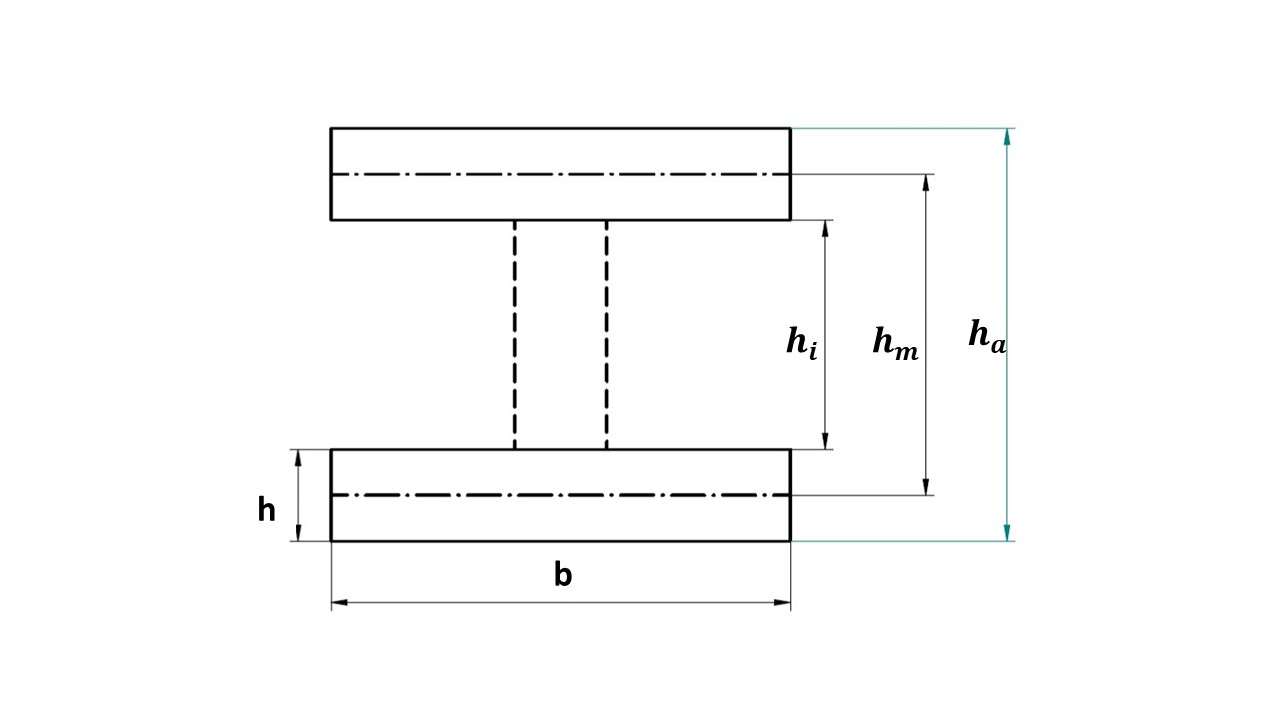
\includegraphics[width=1.0\textwidth]{Bilder/RechteckHolm.jpg}
	\caption{Maße des rechteckigen I-Holms}
	\label{fig: Rechteckholm}
\end{figure}

Bei der Auslegung der Gurte auf Steifigkeit wird angenommen, dass der Steg des I-Trägers keine Längskräfte aufnimmt und der Biegung nicht entgegenwirken kann. Die in der Balkenberechnung ermittelte Biegesteifigkeit $ EI_{x} = 952,55 Nm^{2} $, die erforderlich ist, damit bei einer Kraft $ F_{pruef}=100N $ die Flügelspitze eine Absenkung von $ w_{j=1,1}=20mm $ erfährt, muss allein durch die Gurte aufgebracht werden. Im Sinne der kraftflussgerechten Gestaltung sollen die Glasfasern unidirektional in Längsrichtung des Gurtes angeordnet werden. Die Bezeichnungen der Längenangaben des Holmes orientieren sich an Abb.~\ref{fig: Rechteckholm}~.\\



\noindent Die Gurte werden zur Bestimmung der notwendigen Lagenanzahl als rechteckig angenommen, erst in einem späteren Schritt soll die Form der Kontur der vorgegebenen Haut angepasst werden. Die Maße sind über die gesamte Länge des Holms als konstant anzusehen.\\
Zur Bestimmung des Flächenträgheitsmomentes $ I_{x} $ wird der E-Modul in Längsrichtung der Fasern nach der Mischungsregel nach [3] berechnet.\\
\begin{equation}
 E_{11}=  \phi*E_{f,11}+\left( 1-\phi \right) * E_{M}
\end{equation}
Mit den gegebenen Materialkennwerten bestimmt sich $ E_{11} = 31580 MPa $. Damit ergibt sich ein benötigtes Flächenträgheitsmoment von $ I_{x} = 3,01631 * 10^{-8} m^{4} $.\\

\noindent Das Flächenträgheitsmoment der Gurte bestimmt sich aus den Flächenträg-heitsmomenten der beiden Rechteckquerschnitte und ihren zugehörigen Steiner-Anteilen.
\begin{equation}
	\label{Ix}
	I_{x}=2*\left(\frac{b*h^{3}}{12}+b*h*\left(\frac{h_{m}}{2}\right)^{2}\right)
\end{equation}

\noindent Es wird nach einer Kombination aus Gurtbreite $ b $ und Gurthöhe $ h $ gesucht, die die Anforderungen an das Flächenträgheitsmoment erfüllt, aber dennoch zu einer möglichst geringen Gurtquerschnittsfläche und damit zu einer möglichst geringen Masse der Gurte führt. Um die Steiner-Anteile der Gurte zu maximieren, sollen die Gurte in einem möglichst großen Abstand zur neutralen Faser angeordnet werden. Vorgegeben ist eine Profildicke von $ 37,5mm $, allerdings muss berücksichtigt werden, dass die nach innen gelegte Haut, die Wölbungsrücklage und die Dickenrücklage die maximale Höhe des Holmes einschränken. Deshalb wird die gesamte Gurthöhe auf $ h_{a}=36mm $ abgeschätzt.\\ 

\noindent Die nachstehende Tabelle ~\ref{bh} enthält Werte der Gurtquerschnittsfläche bei verschiedenen Kombinationen von $ b $ und $ h $, die zu einem gesamten Flächenträg-heitsmoment von $ I_{x} = 3,01631 * 10^{-8} m^{4} $ führen.\\
\begin{table}
	\caption{Verschiedene Kombinationsmöglichkeiten von $ b $ und $ h $}
	\label{bh}
	\begin{center}
		\begin{tabular}{l|c|r}
			$h$&$b$&$2*b*h$\\
			\hline
			$1mm$&$38,3mm$&$76,6mm^{2}$\\
			$1,25mm$&$31,1mm$&$77,7mm^{2}$\\
			$1,5mm$&$26,3mm$&$78,8mm^{2}$\\
			$2,25mm$&$18,3mm$&$82,3mm^{2}$\\
		\end{tabular}
	\end{center}
\end{table}



\noindent Den Daten ist zu entnehmen, dass breite Gurte geringer Dicke bei gleichem Flächenträgheitsmoment geringere Querschnittsflächen aufweisen. Aus diesem Grund sollen die Gurte möglichst breit gewählt werden. Die Breite der Gurte ist durch die vorgegebene Konstruktion der Platte zur Aufnahme der Tragfläche am Teststand begrenzt. Die vorgesehene Aussparung weist eine Breite von $ 30mm $ auf. Für die weitere Berechnung soll $ b=28mm $ gelten. Diese Annahme wird dadurch begründet, dass die Fertigung des Holms im Bereich des Modellbaus von Hand erfolgen würde, womit nur grobe Toleranzen einhaltbar sind.\\

\noindent Mithilfe eines Solvers bestimmt sich aus dem Flächenträgheitsmoment und der Gurtbreite die Gurthöhe $ h=1,845mm $.\\
\noindent Im nächsten Schritt wird die zu stapelnde Lagenanzahl ermittelt. Als unidirektionales Material steht das Glasgewebe Interglas 92145 mit einem Flächengewicht von $ 220\frac{g}{m^{2}} $zur Verfügung. Nach [3] berechnet sich die Lagenanzahl $ n $ für eine Dicke des Verbundes $ t_{soll} $ zu:\\

\begin{equation}
	\label{gurtlagen}
	n=t_{soll}*\frac{\phi*\rho_{f}}{\left(\frac{m_{f}}{L*b}\right)}
\end{equation}

\noindent Mit $ \left(\frac{m_{f}}{L*b}\right) = 220\frac{g}{m^{2}} $ und $ t_{soll}=h $ ergibt sich $ n=8,55 $. Es sind also 9 Lagen des Gewebes 92145 für jeden Gurt vorzusehen.Die sich aus 9 Lagen ergebende Gurthöhe kann durch Umstellen von Gleichung ~\ref{gurtlagen} zu $ \tilde{h}=1,941mm $ bestimmt werden. Für den zunächst angenommenen Fall von Gurten mit rechteckigen Querschnitten ist die Auslegung zur Einhaltung der Anforderungen an die Steifigkeit damit abgeschlossen.\\



\subsection{Nachrechnung der angepassten Gurte}
 Die Modellierung der Haut und der Holmgurte in einem CAD-Programm zeigt, dass die Gurte mit den berechneten Bemaßungen nicht innerhalb des Profils mit der als $ 0,75mm $ dick angenommenen Haut liegen. Die Anpassung der Konstruktion der Gurte erfolgt so, dass sich die Gurtoberseite der Innenseite der Haut anschmiegt.Die Gesamtbreite von $ 28mm $, sowie die Gurtdicke bleiben dabei gleich. Da die Wölbungsrücklage ungleich der Dickenrücklage ist, muss die Gesamthöhe $ h_{a} $ auf $ \tilde{h_{a}}=35,8mm $ leicht verringert werden. Abbildung ~\ref{KrummerGurt} veranschaulicht die gekrümmte Form des oberen Holmgurtes.\\
 \begin{figure}
 	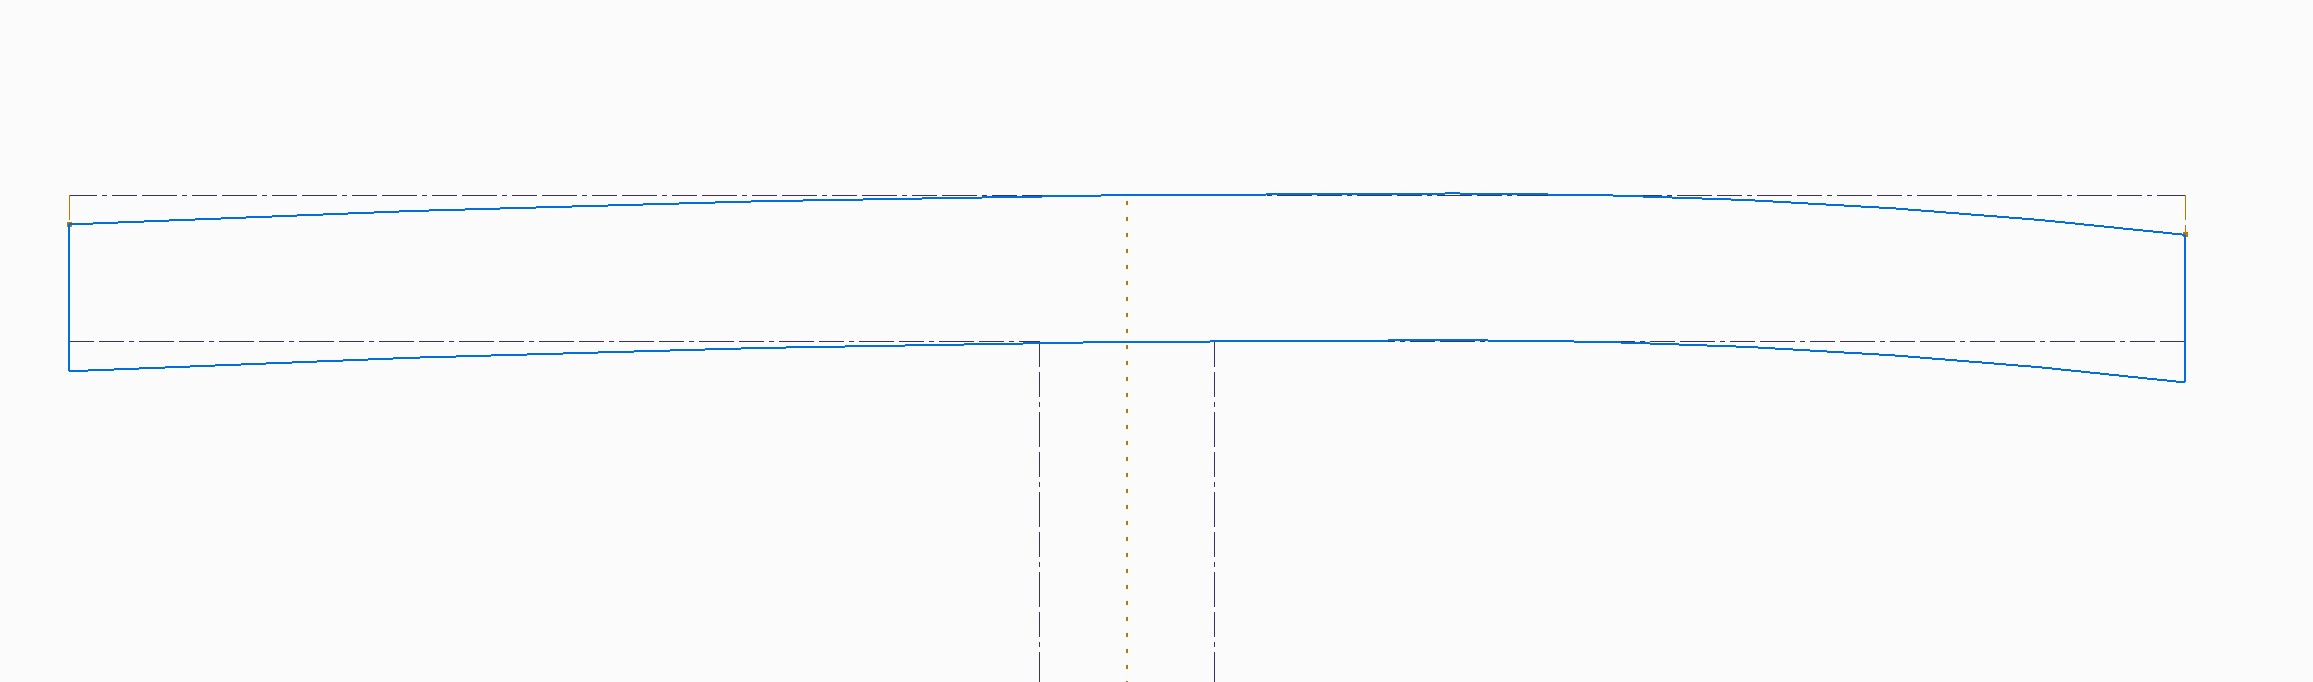
\includegraphics[width=1.0\textwidth]{Bilder/KrummerGurt.jpg}
 	\caption{Der rechteckige Gurt ist gestrichelt dargestellt, der angepasste gekrümmte Gurt mit einer durchgezogenen Linie.}
 	\label{fig: KrummerGurt}
 \end{figure}

\noindent Die angepasste Krümmung der Gurte führt zu einem veränderten Flächenträg-heitsmoment $ \tilde{I_{x}} $ des Balkens, dass mithilfe des CAD-Programms exakt zu $ \tilde{I_{x}}=3,075406*10^{-8}m^{4} $ bestimmt werden kann. Da $ 3,075406*10^{-8}m^{4} > 3,01631*10^{-8}m^{4} $ ist, genügen auch die veränderten Gurte der Steifigkeitsanforderung.\\
 
\noindent Abschließend wird gezeigt, dass die Festigkeit der Gurte einer Belastung der Flügelspitze durch $ F_{pruef}=500N $ standhält. Die aus der Biegung resultierenden und betragsmäßig gleichen Zug- und Druckspannungen werden dazu mit den vorhandenen UD-Festigkeitskennwerten des Handlaminats verglichen. Die Resultate der Balkenberechnungen zeigen, dass das maximale Biegemoment im Holm an Punkt C auftritt und $ M^{b}=500N*0,773m=386,5Nm $ beträgt.In den Randfasern der Gurte resultieren Spannungen, die sich nach\\
\begin{equation}
	\sigma_{b}=\frac{M_{b}*\tilde{h_{a}}}{\tilde{I_{x}}*2}
\end{equation} 
zu $ \sigma_{b}=224,96MPa $ berechnen. Da $ \sigma_{b}< R^{(+)}_{||}=597,9 MPa < R^{(-)}_{||}=650,0 MPa $, ist der Festigkeitsnachweis erbracht. Es kann davon ausgegangen werden, dass die Gurte bei einer Prüfkraft von $ F_{pruef}=500N $ nicht versagen. \\

\subsection{Bestimmung der Lagenanzahl des Steges}
Die Auslegung des Steges erfolgt auch anhand der VDI 2013. Dabei muss beachtet werden, dass der Steg sowohl durch Schubkräfte als auch durch Normalkräfte senkrecht und parallel zu den Gurten Belastungen erfährt. Die Dehnungen der Innenseiten der Gurte werden dem Steg aufgeprägt, da beide Bauteile stoffschlüssig miteinander verbunden sind. Anders als in der VDI 2013 wird jedoch nicht die Bruchdehnung der Gurte betrachtet, sondern die Dehnungen der Innenseiten bei einer Prüfkraft von 500N. So soll die Dimensionierung des Steges auf die Anforderungen an die Festigkeit angepasst werden, um Leichtbaupotentiale bestmöglich auszuschöpfen.\\

\noindent Die größte Längsdehnung der Gurte tritt an der Stelle C auf, da dort das größte Biegemoment wirkt. Sie lässt sich für die Innenseite der Gurte durch
\begin{equation}
	\epsilon_{Gurt}=\frac{\sigma_{innen}}{E_{11}}=\frac{\frac{F_{pruef}*l_{3}*h_{i}}{\tilde{I}_{x}*2}}{E_{11}}
\end{equation}  
 zu $ \epsilon_{Gurt}=6,351*10^{-3} $ berechnen. Auf der Zugseite ist die Dehnung positiv, auf der Druckseite negativ. Die dem Steg aufgeprägte Dehnung führt in Längsrichtung des Steges zu einem Normalkraftfluss, der sich nach VDI 2013 mit
 \begin{equation}
 	p_{\epsilon}=n*\bar{q}*K_{Ex}*\epsilon_{Gurt}
 \end{equation} 
ermitteln lässt. $ K_{Ex} $ ist dabei ein verallgemeinerter Dimensionierungskennwert, der Tafel 3 der VDI 2013 zu $ K_{Ex}=1150*10^{3}m $ entnommen wird. Die Dimensionierungskennwerte der VDI sind nur für bestimmte Verbunde als exakt anzusehen, dennoch liefern sie für die Vorauslegung hinreichend genaue Werte, die in einem späteren Schritt mithilfe eines Laminatrechners überprüft werden können.\\

\noindent Es ist zu beachten, dass in der VDI mit veralteten Einheiten, wie dem Kilopond, gerechnet wird. Flächengewichte $ \bar{q} $ sind durch Multiplikation der auf die Fläche bezogene Masse $ \frac{m_{f}}{L*b} $ mit der Erdbeschleunigung $ \vec{g} $ zu ermitteln. $ n $ kennzeichnet erneut die Lagenanzahl.\\

\noindent Zur kraftflussgerechten Gestaltung des Steges werden die Gewebelagen unter einem Winkel von $ 45^{\circ} $ zu den Holmgurten angeordnet. Deshalb muss die Belastung parallel zu den Fadenrichtungen mithilfe einer Transformationsformel nach VDI 2013 berechnet werden.
\begin{equation}
	p_{\epsilon||}=p_{\epsilon}*cos^{2}\left(45^{\circ} \right)=p_{\epsilon}*0,5 
\end{equation}

Die Normalkräfte an den Gurten bilden im Allgemeinen einen Winkel $ \neq180^{\circ} $ zueinander, da der Holm eine Absenkung erfährt. Daraus resultiert eine Normalkraft auf den Steg, die senkrecht zu den Gurten steht. Diese Abtriebskraft berechnet sich nach VDI 2013 zu:
\begin{equation}
	p_{A}=\frac{2*F_{pruef}*l_{3}*\epsilon_{Gurt}}{h_{m}^{2}}
\end{equation}
 Mit der oben genannten Transformationsformel ergibt sich die Belastung in Faserrichtung.
 \begin{equation}
 	p_{A||}=p_{A}*cos^{2}\left(45^{\circ} \right)
 \end{equation} 

Darüber hinaus erfährt der Steg einen Schubkraftfluss durch den Querkraftschub. Wegen der vernachlässigbaren Längskraftaufnahme des Steges im Vergleich zu den Gurten, kann der Querkraftschub über die Höhe des Steges als konstant angenommen werden. Es muss berücksichtigt werden, dass die Modellierung des Holmes als Balken, der an zwei Punkten gelagert ist und durch die Querkraftbolzen eine weitere Kraft erfährt, zu einem anderen Querkraftverlauf führt als dem konstanten, der in der Richtlinie für den Kragbalken angenommen wurde. Den Berechnungen des Holms als Balken kann eine maximale Querkraft von $ 5085,5N $ im Bereich $ 2 $ und eine maximale Querkraft von $ 500N $ im Bereich $ 3 $ entnommen werden. Mit dem Ziel, im langen Bereich $ 3 $ Gewicht einzusparen, ist es vorteilhaft diesen Bereich geringer Querkraft getrennt von den höher beanspruchten Bereichen $ 1 $ und $ 2 $ auszulegen. Die resultierende Druckbeanspruchung berechnet sich mithilfe der folgenden Formel.
\begin{equation}
	p_{s||}=p_{s}=\frac{Q}{h_{i}}
\end{equation}
Der Kraftfluss, der durch den Steg aufgenommen werden muss, ergibt sich aus der Überlagerung der drei Kraftflüsse $ p_{s||}, p_{A||}, p_{\epsilon||} $. Die Tragfähigkeit einer Schicht des Verbundes wird durch $ K_{\sigma d} $ charakterisiert und kann ebenfalls Tafel 3 der VDI entnommen werden.Da ein Teil der Schubbeanspruchung durch die Matrix geleitet wird, besteht die Gefahr eines Zwischenfaserbruches. VDI 2013 schlägt deshalb die Verwendung von $ K_{\sigma d}=30*10^{3}m $ vor.  Zusätzlich muss der Anteil der Glasmengen in Kette und Schuß durch den Faktor $ k_{||} $ berücksichtigt werden. Das zur Verfügung stehende Gewebe Interglas 90070 hat annähernd gleiche Fadenanzahlen in Kette- und Schußrichtung, damit ist $ k_{||}=0,5 $. 
\begin{equation}
	n*\bar{q}*K_{\sigma d}*k_{||}=p_{s||}+p_{A||}+p_{\epsilon||}
\end{equation}
Die Anzahl der notwendigen Gewebelagen n im Steg lässt sich nun durch Umstellen der Gleichungen und Einsetzen der bekannten Werte ermitteln.\\
\begin{equation}
	n=\frac{\frac{2*F_{Pruef}*l_{3}*\epsilon_{Gurt}}{h_{m}^{2}*2}+\frac{Q}{h_{i}}}{\bar{q}*\left(k_{||}*K_{\sigma d}-K_{Ex}*\epsilon_{Gurt}*0,5\right)}
\end{equation}
Damit ergibt sich die Lagenanzahl von $ n\left(500N\right)=1,99 $ für den Bereich $ 3 $ und $ n\left(5085,5N\right)=18,13 $ für die Bereiche $ 1 $ und $ 2 $. Um einen symmetrischen Lagenaufbau zu ermöglichen, sind also $ 2 $ Lagen für den Bereich $ 3 $ und $ 20 $ Lagen für die Bereiche $ 1 $ und $ 2 $ vorzusehen.\\

\noindent Es ist zu betonen, dass diese Lagenanzahlen maßgeblich durch die Annahmen der Dimensionierungskennwerte $ K_{Ex} $ und $ K_{\sigma d} $ beeinflusst werden. 

\newpage
\section{Auslegung nach CLT}
\subsubsection{Beispielrechnung nach Klassischer Laminattheorie (T.B.)}
Nachdem im Kapitel \ref{CLT} eine Einführung in die klassische Laminattheorie gegeben wurde, wird im Folgenden eine Beispiel-Berechnung eines Lagenaufbaus vorgestellt. Diese beginnt mit den Materialdaten der verwendeten Faser und Matrix und führt bis zu den resultierenden Ingenieurskonstanten. Als repräsentatives Beispiel wird ein Laminat aus zwei Lagen Interglas 92145 mit einer Faserwinkeldifferenz von $\Delta\alpha =90°$ gewählt. Wie zuvor wird auch hier der Faservolumengehalt $\varphi = 40\%$ genutzt, sodass die Gesamtdicke sich zu $t= 2\cdot 0,216mm=0,432mm$ nach den Formel \ref{Dicke}. \\

\noindent Anhand der gegebenen Aufgabenstellung sind Materialdaten der Fasern und der Matrix gegeben, die nachfolgend benötigt werden:\\

\begin{tabular}{ll|ll}
	\multicolumn{2}{c}{Fasermaterial} &\multicolumn{2}{c}{Matrixmaterial}\\
	\hline
	$\rho_{f}$ & $2,55 \frac{g}{cm^{3}}$  & $\rho_{m}$ & $1,18 \frac{g}{cm^{3}}$\\
	\hline
	$E_{f,\parallel}$ & $74000MPa$  & $E_{m}$ & $3300MPa$\\
	\hline
	$E_{f,\perp\perp}$ & $74000MPa$  &  & - \\
	\hline
	$G_{f,\parallel\perp}$ & $30800MPa$ &  & - \\
	\hline
	$\nu_{f,\perp\parallel}$ & $0,2$  &$\nu_{m}$ &  $0,35$\\
\end{tabular}\\

\noindent Da es sich dabei nur um rein isotrope Materialien handelt, gelten $\nu_{f,\perp\parallel} = \nu_{f,\parallel\perp}$ und $G_{f,\parallel\perp} = G_{f,\perp\parallel}$. Der Schubmodul der Matrix berechnet sich zu
\begin{equation}
 	G_{m}=\frac{E_{m}}{2\cdot (1+\nu_{m})}=1222MPa
\end{equation}.\\

\noindent Nun werden anhand der Mischungsregel, jedoch ohne eine Beachtung von Querkontraktionsbehinderungen der Matrix durch die Fasern, Kennwerte einer einzelnen Lage Interglas 92145 bestimmt:

\begin{equation}
	\rho=\rho_{F}\cdot\varphi +\rho_{M}\cdot (1-\varphi)=1,728\frac{g}{cm^{3}}
\end{equation}
\begin{equation}
	E_{\parallel}=E_{f,\parallel}\cdot \varphi+E_{m}\cdot (1-\varphi)=31580 MPa
\end{equation}
\begin{equation}
	E_{\perp}=\frac{E_{f,\perp}\cdot E_{m}}{E_{m}\cdot \varphi+E_{f,\perp}\cdot (1-\varphi)}=5341MPa
\end{equation}
\begin{equation}
	\nu_{\perp\parallel}=\nu_{f,\perp\parallel}\cdot\varphi+\nu_{m}\cdot(1-\varphi)=0,29
\end{equation}
\begin{equation}
	\nu_{\parallel\perp}=\nu_{\perp\parallel}\cdot\frac{E_{\parallel}}{E_{\perp}}=0,049
\end{equation}\\

\noindent Mit diesen Moduln und Querkontraktionszahlen wird im weiteren die Steifigkeitsmatrix des gesamten Laminats, transformiert in Koordinatensystem-Hauptrichtungen $x$ und $y$, bestimmt. Begonnen wird mit der Steifigkeitsmatrix einer einzelnen Gewebelage, bezogen wird sich auf dessen Faserrichtung. Damit kann  
\begin{equation}
	\underline{\sigma}=\underline{\underline{Q}} \cdot \underline{\epsilon}
\end{equation}\\aufgestellt werden. Bei den Steifigkeitsmatrix $\underline{\underline{Q}}$ handelt es sich um Scheiben-Steifigkeiten.

\begin{equation}
\underline{\underline{Q}}=
\begin{bmatrix}
	\frac{E_{\|}}{1-\nu_{\perp \|}\cdot \nu_{\| \perp}}&	\frac{\nu_{\| \perp}\cdot E_{\|}}{1-\nu_{\perp \|}\cdot \nu_{\| \perp}}&0\\
	
	\frac{\nu_{\perp \|}\cdot E_{\perp}}{1-\nu_{\perp \|}\cdot \nu_{\| \perp}}&\frac{E_{\perp}}{1-\nu_{\perp \|}\cdot \nu_{\| \perp}}&0\\
	
	0&0&G_{\perp\parallel}
\end{bmatrix} =
\begin{bmatrix}
	32035 & 1570 & 0\\
	1570 & 5418 & 0\\
	0 & 0 & 1985
\end{bmatrix} [MPa]
\end{equation}\\

\noindent Bevor die einzelnen Lagen in ihrer Wirkung zusammengefasst werden können, müssen sie der Ausrichtung entsprechend um den Faserwinkel rotiert werden:

\begin{equation}
	\underline{\underline{T}}=
	\begin{bmatrix}
		\cos^{2}\alpha&\sin^{2}\alpha&-\sin 2\alpha\\
		\sin^{2}\alpha&\cos^{2}\alpha&\sin 2\alpha\\
		0,5\cdot \sin2\alpha&-0,5\cdot\sin2\alpha&\cos 2\alpha
	\end{bmatrix}
\end{equation}\\

\noindent Somit lauten die neuen Steifigkeitsmatrizen nach 
\begin{equation}
	\overline{\underline{\underline{Q}}}=\underline{\underline{T}}\cdot \underline{\underline{Q}} \cdot \underline{\underline{T}}^{T}  
\end{equation}\\

\begin{equation}
\underline{\underline{\overline{Q}_{k=1}}}=
\begin{bmatrix}
	32035 & 1570 & 0\\
	1570 & 5418 & 0\\
	0 & 0 & 1985
\end{bmatrix} [MPa], \alpha = 0°
\end{equation}\\
\begin{equation}
	\underline{\underline{\overline{Q }_{k=2}}}=
	\begin{bmatrix}
		5418 & 1570 & 0\\
		1570 & 32035 & 0\\
		0 & 0 & 1985
	\end{bmatrix} [MPa], \alpha = 90°
\end{equation}\\

\noindent Mittels dessen einzelnen Werten $\overline{Q}_{ij, k}$ lassen sich der Scheiben-, der Koppel- und der Plattenquadrant des Mehrschichtverbundes berechnen. In diesem können die Berechnungen teilweise vereinfacht werden, da die beiden Lagendicken $t_{k}$ dem Betrag der Abstände $|z_{k}|$ entspricht.

\begin{equation}
	A_{ij}= \sum_{k=1}^{2} \overline{Q}_{ij,k}\cdot t_{k}
\end{equation}
\begin{equation} \underline{\underline{A}}=
	\begin{bmatrix}
		8090,1 & 678,8 & 0\\
		678,8 & 8090,1 & 0\\
		0 & 0 & 857,3\\
	\end{bmatrix} \Bigl[\frac{N}{mm}\Bigr]
\end{equation}


\begin{equation}
	B_{ij}= \cdot \sum_{k=1}^{2} \overline{Q}_{ij,k}\cdot t_{k}\cdot \left(z_{k}-\frac{t_{k}}{2}\right)
\end{equation}
\begin{equation} \underline{\underline{B}}=
	\begin{bmatrix}
		620,9 & 0 & 0\\
		0 & -620,9 & 0\\	
		0 & 0 & 0\\
	\end{bmatrix} [N]
\end{equation}

\begin{equation} 
	D_{ij}=\sum_{k=1}^{2} \overline{Q}_{ij,k}\cdot \left(\frac{t_{k}^{3}}{12}+t_{k}\left(z_{k}-\frac{t_{k}}{2}\right)^{2}\right)
\end{equation}
\begin{equation}\underline{\underline{D}}=
	\begin{bmatrix}
		125,8 & 10,6 & 0\\
		10,6 & 125,8 & 0\\
		0 & 0 & 13,3
	\end{bmatrix} [Nmm]
\end{equation}\\

\noindent Aus diesen Matrizen lässt sich nun das \textit{ Elastizitätsgesetz des kombinierten Scheiben-Plattenelements} anwenden:

\begin{equation}
	\begin{pmatrix}
		\hat{\underline{n}}\\
		\hat{\underline{m}}
	\end{pmatrix}
	= \begin{bmatrix}
		\underline{\underline{A}}&\underline{\underline{B}}\\
		\underline{\underline{B}}&\underline{\underline{D}}
	\end{bmatrix}
	\cdot \begin{pmatrix}
		\underline{\epsilon}\\
		\underline{\kappa}
	\end{pmatrix}
\end{equation}\\

\noindent Damit kann für jede einzelne Lage das Festigkeitskriterium nach Puck überprüft werden. Eine Fortsetzung der Beispielrechnung mittels dieses Festigkeitskriteriums wird ab dieser Stelle nicht mehr durchgeführt, da sie bis auf wenige Ausnahmen nicht mehr analytisch zu lösen ist.\\

\noindent Mit der Inversen der Scheibenmatrix $\underline{\underline{A^{-1}}}$ werden abschließend die Ingenieurskonstanten des Mehrschichtverbundes ohne Querkontraktionsbehinderung ermittelt:

\begin{equation}
	\hat{E}_{x}=\frac{1}{A_{11}^{-1}\cdot t} = 18727 MPa
\end{equation}
\begin{equation}
	\hat{E}_{y}=\frac{1}{A_{22}^{-1}\cdot t} = 18727 MPa
\end{equation}
\begin{equation}
	\hat{G}_{xy}=\frac{1}{A_{66}^{-1}\cdot t} = 1984,5 MPa
\end{equation}
\begin{equation}
	\hat{\nu}_{xy}=-\frac{A_{12}^{-1}}{A_{22}^{-1}} = 0,084
\end{equation}
\begin{equation}
	\hat{\nu}_{yx}=-\frac{A_{12}^{-1}}{A_{11}^{-1}} = 0,084
\end{equation}


\subsubsection{$eLamX^{2}$ (T.B.)}\label{elamx}
$eLamX^{2}$ ist ein Laminat-Berechnungsprogramm der TU Dresden. Es kann anhand der klassischen Laminattheorie mit unterschiedlichen Versagenskriterien berechnen, inwiefern ein gewählter Lagenaufbau den Festigkeitskriterien gerecht wird. Zusätzlich sind weitere Funktionen, wie zum Beispiel Beulberechnungen, Optimierungen etc. nutzbar und andere Einflüssse, z.B. Temperatureinflüsse anwendbar, jedoch für diese Auslegung irrelevant.

\noindent Auch hier wurden vorerst die gegeben Materialeigenschaften der Aufgabenstellung als Fasermaterial, Matrixmaterial und  UD-Festigkeitskennwerte definiert (Anmerkung: In $eLamX^{2}$ wird bei der Indizierung die Notierung \glqq Ursache - Wirkung\grqq\: statt \glqq Wirkung - Ursache\grqq\: verwedet). )\\

\begin{tabular}{ll|ll|ll}
	\multicolumn{2}{c}{Fasermaterial} &\multicolumn{2}{c}{Matrixmaterial}  &\multicolumn{2}{c}{UD-Festigkeitskennwerte} \\
	\hline
	$\rho_{f}$ & $2,55 \frac{g}{cm^{3}}$  & $\rho_{m}$ & $1,18 \frac{g}{cm^{3}}$  & $R_{\parallel}^{+}$ & $597,9MPa$ \\
	\hline
	$E_{f,\parallel}$ & $74000MPa$  & $E_{m}$ & $3300MPa$  & $R_{\parallel}^{-}$ & $650,0MPa$\\
	\hline
	$E_{f,\perp\perp}$ & $74000MPa$  &  &   & $R_{\perp}^{+}$ & $37,7MPa$\\
	\hline
	$G_{f,\parallel\perp}$ & $30800MPa$ & $G_{m}$ & $1222MPa$ & $R_{\perp}^{+-}$ & $130,0MPa$\\
	\hline
	$\nu_{f,\perp\parallel}$ & $0,2$  &$\nu_{M}$ &  $0,35$  & $R_{\parallel\perp}$ & $37,5MPa$\\
\end{tabular}\\

\noindent Mit einem Faservolumenanteil $\varphi=0,4$ ergeben sich folgende weitere Materialeigenschaften:\\

\begin{tabular}{ll}
	$\rho$ & $1,728 \frac{g}{cm^{3}}$ \\
	\hline
	$E_{\parallel}$ & $31580 MPa$\\
	\hline
	$E_{\perp}$ & $5341,2MPa$\\
	\hline
	$\nu_{\parallel\perp}$ & $0,29$\\
	\hline
	$G_{\parallel\perp}$ & $1984,5 MPa$\\
\end{tabular}\\

\noindent Anschließend werden die nach Kapitel ~\ref{VDI2013} berechneten Laminate bzw. Schichtverbunde aus mehreren Gewebe-Lagen zusammengesetzt. Eine bidirektionale Gewebelage wird dabei durch zwei einzelne Materiallagen mit einem Winkel von $90^{\circ}$ zueinander simuliert, sodass sich die doppelte Anzahl des Materials gegenüber der Gewebeanzahl ergibt. Für die Holmgurte ergibt sich ein Lagenaufbau nach Abbildung ~\ref{fig:Lagenaufbau Holmgurte} und für den dünnen Steg nach Abbildung ~\ref{fig:Lagenaufbau Steg dünn}. Für den dicken Steg ergibt sich der gleiche Aufbau wie bei dem dünnen Steg, allerdings mit 24 Materiallagen (siehe Abb. ~\ref{fig:Lagenaufbau Steg dick}). Weshalb sich die Anzahl der Gewebelagen gegenüber der Auslegung nach VDI 2013 unterscheidet, wird im Weiteren beschrieben.\\ 

\noindent Anschließend werden die nach VDI 2013 im Kapitel \ref{VDI} errechneten Normalkraft- und Schubflüsse bzw. Dehnungen eingegeben, sodass nun die Sicherheiten nach den Versagenskriterien von Puck ermittelt werden können. Dabei handelt es sich um leicht abweichende Flüsse bzw. Dehnungen gegenüber der Realität. Diese Werte stammen aus der Auslegung nach VDI 2013, in der teilweise die Lagenanzahl, wie bereits beschrieben, geringer ist. Zu beachten ist außerdem, dass die Flüsse und Dehnungen auf das allgemeine Koordinatensystem und nicht auf die der einzelnen Lagen bezogen werden. Es wird automatisch die niedrigste Sicherheit mit der jeweiligen Versagensart ausgegeben. Auch muss berücksichtigt werden, dass für die komplette Überprüfung der Auslegung ebenfalls $\epsilon_{x}$ negativ angenommen werden muss, um den gegenüberliegenden Gurt mit Druckbelastungen zu betrachten. Dabei ergeben sich jedoch stets höhere Sicherheiten.\\

\noindent Um immer eine Sicherheit von $j>1$ zu garantieren, müssen im Steg nachträglich noch weitere Lagen zu der ursprünglich berechneten Anzahl hinzugefügt werden, sodass sich eine Gesamt-Lagenanzahl von 4 und 24 statt 2 und 20 ergibt. Diese Abweichung kann u.a. daran liegen, dass die VDI 2013 mit Konstanten rechnet, die nur beispielhaft an einem Gewebe ermittelt wurden und somit nicht exakt für die gegebenen Gewebe der Aufgabenstellung gelten können. Außerdem kann der Einfluss, dass lediglich mit der einfachen Mischungsregel ohne Querkontraktionsbehinderung der Matrix gerechnet wurde, eine leichte Abweichung gegenüber anderen Berechnungsmethoden verursachen.
Dargestellt sind die Rechnungen in Abb. ~\ref{fig:Berechnung Holmgurte}, Abb.~\ref{fig:Berechnung Steg dünn} und Abb.~\ref{fig:Berechnung Steg dick}.\\

\noindent Als nächstes können die Ingenieurskonstanten (E-Moduln des gesamten Laminats in Hauptachsenrichtungen) ermittelt werden, welche für die spätere Stabilitätsabschätzung benötigt werden (siehe Abb. ~\ref{fig:Ingenieurskonstanten Holmgurte}, Abb. \ref{fig:Ingenieurskonstanten Steg dick} und Abb.~\ref{fig:Ingenieurskonstanten Steg dünn}).\\

\noindent Der Übersichtlichkeit halber werden die Abbildung im Kapitel \ref{Abbildungen} dargestellt.
\newpage
\section{Beulabschätzung des Holms}
\input{Projektarbeit - Beulabschätzung des Holms}
\newpage
\section{Auslegung der Klebeverbindung}
Als letzte analytische Auslegung sollen die Klebeflächen berechnet werden.
\subsection{Klebeverbindung Steg - Gurt (T.B.)}
Die Klebverbindung wird ähnlich der [VDI 2013]  ausgelegt, sodass nur die Abtriebskraft des Holms und die übertragene Querkraft den Schubfluss für die Belastung definieren:
\begin{equation}
	p=\sqrt{p_{A}^{2}+p_{s}^{2}}
\end{equation}
Die Länge ergibt sich aus 
\begin{equation}
	l=\frac{p}{\tau_{zul}}
\end{equation}
wobei 
\begin{equation}
	\tau_{zul}=7MPa
\end{equation}
nach [Kennwerte Idaflieg] beträgt.\\

\noindent Bereich $I$ und $II$ werden, ähnlich der Beulberechnung, zusammen ausgelegt mit den kritischsten Werten, sodass 
\begin{equation}
	l=\frac{\sqrt{(4282,26\frac{N}{m})^{2}+(159330,16\frac{N}{m})^{2}}}{7\frac{N}{m^{2}}}=22,8mm
\end{equation}
als Klebebreite benötigt werden. Für den Bereich $III$ ergibt sich
\begin{equation}
	l=\frac{\sqrt{(4282,26\frac{N}{m})^{2}+(15665,14\frac{N}{m})^{2}}}{7\frac{N}{m^{2}}}=2,32mm
\end{equation}
Beide Klebebreiten passen auf die verbleibende innere Holmgurtflächen und sollen durch Mumpe ohne zusätzliche Gewebelagen realisiert werden.

\subsection{Klebeverbindung Holm - Rippen (T.B.)}
Die vergrößerten Klebeflächen der Rippen gegenüber dem Holm sollen durch Holzklötze ermöglicht werden, die auf beide Seiten des Stegs zwischen die Holmgurte geklebt werden. Die Breite dieser Klötze errechnet sich aus 
\begin{equation}
	A=\frac{F}{\tau_{zul}}
\end{equation}
mit der maximal abgesetzten Kraft von $F=500N$.
Somit haben die Holzklötze eine Breite von 
\begin{equation}
	b=1,12mm
\end{equation}
bei einer Höhe von $35,8mm-2\cdot 1,941mm$.
\newpage
\section{Bolzenauslegung}


\subsection{Bolzenberechnung}
Zunächst muss eine Auslegung für die Flächenpressung erfolgen. Dabei ist für Buche $\sigma_{p,zul}=60\frac{N}{mm^2}$
Die projizierte Fläche ist $A=a*d$ , d ist hierbei der Durchmesser des Bolzens und a die Länge des Lochs im Steg.\\
Die Flächenpressung ist nun: 
\begin{equation}
	p=\frac{F}{A}=\frac{5085,5\mathrm{N}}{a*8mm}
\end{equation}
Mit der zulässigen Flächenpressung für Buchenholz lässt sich die Gleichung nun nach a auflösen:
\begin{equation}
	a=\frac{F}{\sigma_{p,zul}*d}=\frac{5085,5\mathrm{N}}{60\frac{N}{mm^{2}}*8mm}=10,59mm
\end{equation}
Somit muss die Holzverstärkung des Stegs an der Stelle der Lager mindestens eine Breite von 10,59$\mathrm{mm}$ aufweisen. Im Weiteren wird eine Breite von 11$\mathrm{mm}$ angenommen.\\
 
Nun werden die Bolzen, die den Holm im für den Versuchsaufbau vorgegebenen U-Profil fixieren, ausgelegt. Die Bolzen sind auf Biegung belastet, wodurch sich die Gleichung:
\begin{equation}
	\sigma_{b}=\frac{M_{b}}{W} 
\end{equation}
,ergibt.\\
 Mit: 
 \begin{equation}
 	W_{Kreis}=\frac{\pi*d^{3}}{32}
 \end{equation}
 und 
 \begin{equation}
 	M_{b}=F*l
 \end{equation}
 ergibt sich die Biegespannung zu
 \begin{equation}
 	\sigma_{b}=F*\frac{32*l}{\pi*d^{3}}
 \end{equation}
Die zu ertragende Kraft ist $5085,5 \mathrm{N}$. Diese lässt sich jetzt noch halbieren, da mit der oben genannten Annahme nur die Hälfte des Bolzens betrachtet wird. Damit ergibt sich:
 \begin{equation}
 	F_{bel}=\frac{F}{2} =2542,75 \mathrm{N}
 \end{equation}
 Nun kann mit $d=8mm$ und $l=8,559mm$ ein passendes Material gesucht werden. Für Stahl gilt $\sigma_{b,F}\approx1,2*R_{e}$, somit muss 
 \begin{equation}
 	F*\frac{32*l}{1,2*\pi*d^{3}}=360,8\mathrm{MPa}\leq
R_{e} \end{equation}  sein.\\

 Mit den getroffenden Annahmen ist S620Q (anderer) mit einer Streckgrenze von $R_{e}=620\frac{N}{mm^{2}}$ ein geeigneter Stahl.\cite{item6}\\
 
 
 
 
  
 

\newpage
\section{Schubfluss}

\subsubsection{Theorie (O.S.)}
Im Leichtbau ist es wichtig geeignete Konstruktionen zu entwerfen, um Eigenschaften der Werkstoffe ideal nutzen zu können. Das Gesamtbauteil ist dann meist so kompliziert, dass sich die für das Bauteil zu lösenden Differenzialgleichungen, wie zum Beispiel die der Elastostatik, keine geschlossenen Lösungen finden lassen. Das Ziel ist es nun durch Annahmen und Vereinfachungen ein sinnvolles und lösbares Ingenieursmodell zu finden. Alternativ könnten auch Lösungen mittels numerischer Methoden ermittelt werde, hierzu mehr in Kapitel \ref{FEM}.

\paragraph{Zylindrische, dünnwandige Profile}~\\
Häufig werden zylindrische, dünnwandige Profil genutzt, da sie bei vergleichsweiser niedriger Masse noch immer gut Werte bei zum Beispiel der Biegesteifigkeit liefern. Sie kennzeichnen sich dadurch aus, dass deutlich höhere Ausmaße in x-Richtung haben, als in jede andere (zylindrisch). Eine Laufvariable $s$ verläuft in der y-z-Ebene durch die Mitte der Profildicke $t(s)$. Die Dicke ist nicht zwangsläufig über $s$ konstant, muss aber deutlich kleiner als alle anderen Abmessungen sein (dünnwandig) \cite{item15}. Man kann vereinfacht annehmen
\begin{equation}
	\iint dA=\int t(s)ds.
\end{equation} 
Der Querschnitt muss in x-Richtung konstant sein und auch bei Belastung seine Gestalt beibehalten. Der Schubfluss im Profil ist als
\begin{equation}\label{tau}
	q=\tau t(s)
\end{equation}
und der Normalkraftfluss als
\begin{equation}
	n_x=\sigma_x t(s)
\end{equation}
definiert. Für diese Kraftflüsse gilt das hydrodynamische Analogon. Das heißt mit einer Änderung der Dicke muss der Kraftfluss antiproportional ab- bzw. zunehmen, damit das Kräftegleichgewicht erfüllt bleibt. Für Knotenpunkte muss auch gelten, dass der Betrag der Kraftflüsse in den Knoten hinein denen aus ihm heraus gleichen. Des Weiteren lässt sich noch zwischen offenen und geschlossenen Profilen unterscheiden, wobei es sich bei zweiterem um Ein- oder Mehrzeller handeln kann.\cite{item15}

\paragraph{Koordinatensysteme}~\\
Bei den Berechnungen kann viel Arbeit gespart werden, indem das Koordinatensystem mit Ursprung und Achsenausrichtung klug gewählt wird. Das allgemeine Koordinatensystem, das unabhängig vom betrachteten Profil ist, bietet hierbei die wenigstem um nicht zu sagen keine Vorteile. Verschiebt man seinen Ursprung in den Schwerpunkt erhält man das Schwerpunkt-Koordinatensystem. Es wird mit einem Querstrich über den Koordinaten gekennzeichnet ($\bar{x},\bar{y},\bar{z}$). Hier ergibt sich das Flächenmoment 1. Ordnung  $S$ (siehe Gleichungen \ref{SM1}, \ref{SM2}), auch statisches Moment genannt, über das gesamte Profil zu null.

Aus dem Kräftegleichgewicht an einem infinitesimalen Volumen des dünnwandigen Profils ergibt sich der Zusammenhang zwischen den Kraftflüssen zu
\begin{equation}
	q(s)=-\int\frac{\partial n_x(x,s)}{\partial x}ds+q_0.
\end{equation}
Wird nun der Normalkraftfluss in Abhängigkeit von der Querkraft $Q$ gesetzt, ergibt sich die $Q$-$SI$nen-Formel:
\begin{equation}\label{qs}
	q(s)=-(Q_{\bar{z}}\frac{S_{\bar{y}}(s)I_{\bar{z}}-S_{\bar{z}}(s)I_{\bar{yz}}}{I_{\bar{y}}I_{\bar{z}}-I_{\bar{yz}}^2}+Q_{\bar{y}}\frac{S_{\bar{z}}(s)I_{\bar{y}}-S_{\bar{y}}(s)I_{\bar{yz}}}{I_{\bar{z}}I_{\bar{y}}-I_{\bar{yz}}^2})+q_0
\end{equation}
Mit den Flächenträgheitsmomenten $I$ (siehe Gleichungen \ref{FT1}-\ref{FT3}). Spätestens hier zeigt sich, dass für dieses Modell das Superpositionsprinzip anwendbar ist und man die Kräfte $Q_y$ und $Q_z$ getrennt betrachten kann.
Hier lässt sich direkt erkennen, wie diese Formel durch die Wahl eines besseren Koordinatensystems vereinfacht werden kann. Für das Hauptachsen-Koordinatensystem bleibt der Schwerpunkt weiterhin der Ursprung, jedoch werden die Achsen so um die x-Achse gedreht, dass die Deviationsmomente $I_{yz}$ verschwinden. Es wird mit einem Dach über den Koordinaten gekennzeichnet ($\hat{x},\hat{y},\hat{z}$). Die Integrationskonstante
\begin{equation}
	q_{0} = q_{0b}+q_{0T}
\end{equation}
ist nur bei geschlossenen Profilen ungleich null. Sie sich aus einem Teil, der aus der Biegung entsteht $q_{0b}$ und einem aus der Torsion $q_{0T}$ zusammen. Es gibt einen Punkt in der y-z-Ebene für jedes Profil, wo eine angreifende Kraft keine Torsion verursacht. Dieser Punkt ist von hoher Bedeutung und wir Schubmittelpunkt genannt.
\subsubsection{Idealisierung}
Für die Berechnung des Schubmittelpunkts wird das Flügelprofil als vereinfachter Mehrzeller angenommen.
Dabei wird der Ursprung des Koordinatensystems am unteren rechten Rand gesetzt. Das Modell wird in 10 Teilstrecken $s_{i}$ aufgeteilt. Die Dicke $t$ wird über die Schale konstant angenommen. Der Schaum wird in allen Abschnitten der Schale und im Holm vernachlässigt, da seine Hauptaufgabe der Beulsteifigkeit gilt und er bei der Schubaufnahme im Vergleich zum Laminat nur eine unbedeutende Rolle spielt. Der Steg ist in 2 Abschnitte unterteilt. Für die maximale Belastung und somit für die Auslegung relevant ist nur der Teil mit dem dünneren Gewebe, sodass hier für die Dicke des Stegs $t_{1}=0,314\mathrm{mm}$ angenommen wird. Für die Gurte gilt, dass alle Fasern parallel in x-Richtung ausgerichtet sind. Sie werden in dieser Rechnung ignoriert, da sie folglich im Gegensatz zum $\pm45^\circ$-Gewebe vernachlässigbare Schubkräfte aufnehmen können (D = $t$). Außerdem würde ein über die Dicke variabler Schubmodul die Rechnung unnötig verkomplizieren, da die uns bekannten Methoden zur Schubflussberechnung nur für homogene Werkstoffe gültig sind \cite{item15}.

Diese Annahmen bezüglich des Schaums und der Gurte sind unproblematisch, da sie so getroffen wurden, dass der Flügel sogar noch höheren Belastungen als errechnet standhalten könnte. Als einziges ist zu betrachten, dass durch das Wegfallen des Schaums in der Schale die GFK-Schichten des Sandwichs aufeinander fallen und ihre Position somit um wenige Millimeter ungenau ist. Da die genau errechnete Dicke auf eine Lagenschicht aufgerundet werden muss, ist dies vermutlich kompensierbar, sollte jedoch im Hinterkopf behalten werden.

Abbildung \ref{Fluegel1} zeigt, dass der Profil durch 4 geraden Strecken und einen viertel Kreis modelliert wurde. Die Längen der einzelnen Teilabschnitte lassen sich im Anhang der Abbildung \ref{fig:LaengenS} entnehmen.
\begin{figure}[h]
 \centering
 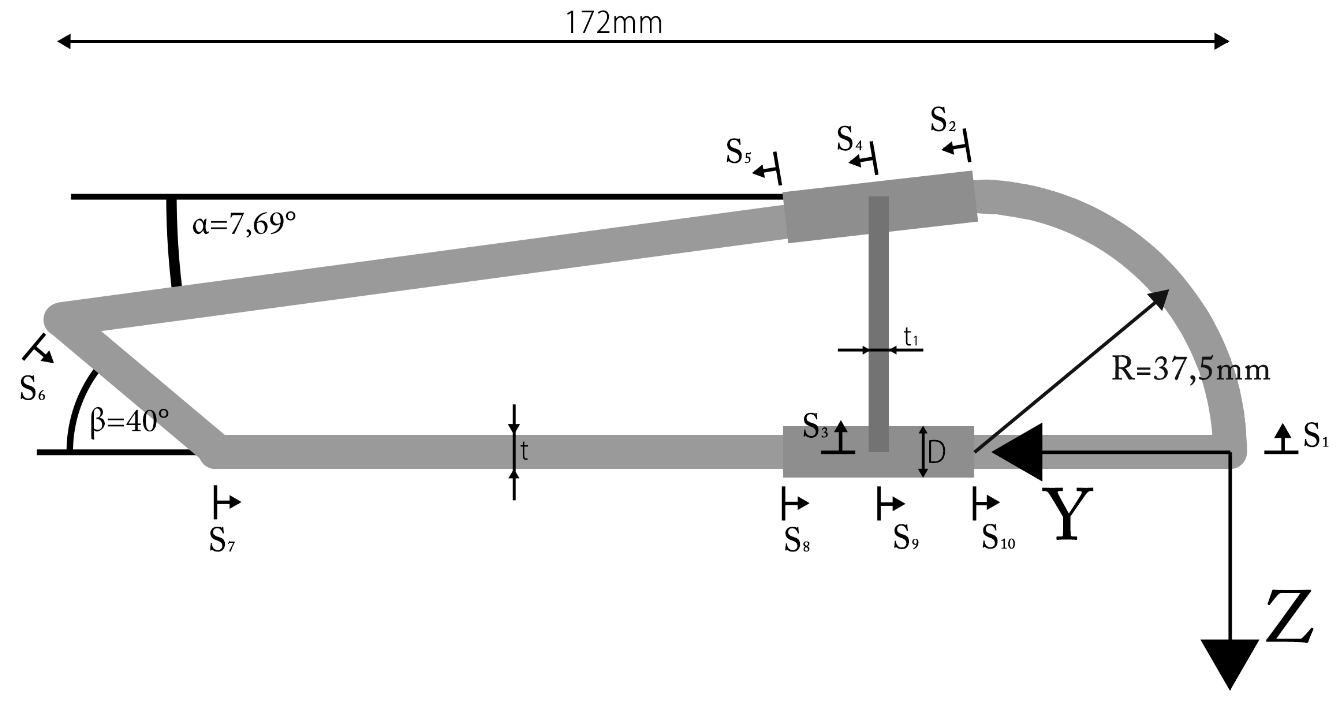
\includegraphics[width=1\textwidth]{Bilder/Model1}
 \caption{vereinfachtes Model}
 \label{Fluegel1}
\end{figure}
\subsubsection{Schwerpunktkoordinaten}\label{SP-Koord}
Zunächst wird von einer Dicke $t=0,2\mathrm{mm}$ ausgegangen und die statischen Momente in den einzelnen Teilstücken berechnet.
\begin{equation}\label{SM1}
	S_{z}=\int_{A}^{}y \mathrm{d}A =t\int_{s}^{}y \mathrm{d}s
\end{equation}
\begin{equation}\label{SM2}
	S_{y}=\int_{A}^{}z \mathrm{d}A =t\int_{s}^{}z \mathrm{d}s 
\end{equation}
Damit ergeben sich für die statischen Momente in $\mathrm{mm}^3$:

\begin{center}
\begin{tabular}[h]{l|c|c}
	
Bauteilabschnitt&$S_{y}/\mathrm{mm}^3$&$S_{z}/\mathrm{mm}^3$\\
\hline
1& -281,25&160,54\\
2&-120,382&124,42\\
3&-220,78&605,24\\
4&-97,13&163,27\\
5&-571,91&2555,63\\
6&-58,13&965,14\\
7&0&1789,88\\
8&0&163,80\\
9&0&124,60\\
10&0&140,63\\
\end{tabular}
\end{center}

\noindent Nun kann aus den statischen Momenten der Schwerpunkt bestimmt werden, indem das Statische Moment über alle Flächen zusammenaddiert wird:
\begin{equation}
	y_{0}=\frac{\int_{s}{}t(s)y\mathrm{d}s}{\int_{s}{}t(s)\mathrm{d}s}=\frac{S_{z}}{A}
\end{equation}
\begin{equation}
	z_{0}=\frac{\int_{s}{}t(s)z\mathrm{d}s}{\int_{s}{}t(s)\mathrm{d}s}=\frac{S_{y}}{A}
\end{equation}
Mit einer Dicke von $t=0,2\mathrm{mm}$ ergeben sich Lagen der Schwerpunktkoordinaten zu:
$$
	y_{0}=78,53\mathrm{mm}
$$
$$
	z_{0}=-15,39\mathrm{mm}
$$

Damit können nun mit
\begin{equation}
	S_{\bar{y}}=S_y-z_0A
\end{equation} 
\begin{equation}
S_{\bar{z}}=S_z-y_0A
\end{equation} 
die Verläufe der statischen Momente in Bezug auf den Schwerpunkt ermittelt werden, wobei die Endwerte der vorherigen Verläufe nach dem hydrodynamischen Analogon den Anfangswert $s_0$ des folgenden Bereichs bestimmen. Dabei ergeben sich folgende Endwerte in $\mathrm{mm}^3$:
\begin{center}
\begin{tabular}[h]{l|c|c}
Bauteilabschnitt&$S_{\bar{y}}/\mathrm{mm}^3$&$S_{\bar{z}}/\mathrm{mm}^3$\\
\hline
1&-99,91&-764,60\\
2&-159,18&-860,06\\
3&-39,53&-319,43\\
4&-252,75&-1236,10\\
5&-493,03&-372,27\\
6&-458,59&120,60\\
7&-201,65&599,69\\
8&-158,55&543,61\\
9&-155,45&448,34\\
10&0&0\\
\end{tabular}
\end{center}
Für ein offenes Profil muss gelten, dass an den freien Rändern das statische Moment $ 0 $ ist. Das Profil wird in diesem Fall an den Stellen 1 und 3 geschnitten. Für die nun freien Enden an den diesen Bereichen wird $s_0=0$ und auch die Endwerte des Bereichs 10 werden zu $0$.

Nun werden die Flächenträgheitsmomente 
\begin{equation}\label{FT1}
	I_{y} = \int_{A}^{}z^2dA
\end{equation}
\begin{equation}
I_{z} = \int_{A}^{}y^2dA
\end{equation}
\begin{equation}\label{FT3}
I_{yz} = \int_{A}^{}zydA
\end{equation}
 zuerst aus ihrem eigenen Schwerpunkt aus errechnet, sodass die auf den Gesamtschwerpunkt bezogenen Flächenträgheitsmomente $I_{\bar{y}}$, $I_{\bar{z}}$ und $I_{\bar{y}\bar{z}}$ mit Hilfe des Steinerschen Satz
 \begin{equation}
 	I_{\bar{y}} = I_{y} + z^2A
 \end{equation}
\begin{equation}
I_{\bar{z}} = I_{z} + y^2A
\end{equation}
\begin{equation}
I_{\bar{y}\bar{z}} = I_{yz} + zyA
\end{equation}
 ermittelt werden können.
Es ergibt sich:
\begin{center}

\begin{tabular}[h]{l|c|c|c||c|c|c}
Bauteilabschnitt&$I_{y}/\mathrm{mm}^4$&$I_{z}/\mathrm{mm}^4$&$I_{zy}/\mathrm{mm}^4$&$I_{\bar{y}}/\mathrm{mm}^4$&$I_{\bar{z}}/\mathrm{mm}^4$&$I_{\bar{y}\bar{z}}/\mathrm{mm}^4$\\
\hline
1&2857,61&2857,61&140,63&5649,01&22688,56&-7299,54\\
2&0,83&44,91&6,06&1255,75&3299,07&2026,88\\
3&1379,88&0,10&0&1512,59&8665,70&1072,37\\
4&0,83&44,91&6,06&1043,48&1189,34&1098,42\\
5&373,09&20459,31&2762,56&3053,01&55094,88&-6871,78\\
6&187,25&265,93&-223,13&284,51&20659,15&2599,67\\
7&0,06&9689,11&0&3955,08&23439,99&7374,62\\
8&0,01&45,731&0&663,45&1168,88&-863,21\\
9&0,01&45,731&0&663,45&3287,88&-1466,61\\
10&0,03&878,91&0&1777,09&27679,54&-6901,18\\
\hline
$\sum{}$&-&-&-&19957,41&187173,00&-9230,37
\end{tabular}
\end{center}
Es kann sofort erkannt werden, dass $I_{\bar{y}\bar{z}} \neq 0$ ist und es sich somit nicht um ein Hauptachensystem handelt. Das Deviationsmoment  $I_{\bar{y}\bar{z}}$ ist jedoch im Vergleich zu den anderen Flächenträgheitsmomenten sehr niedrig. 
Aus dem Zusammenhang
\begin{equation}
	tan(\varphi)=\frac{2I_{\bar{y}\bar{z}}}{I_{\bar{z}}-I_{\bar{y}}}
\end{equation}
lässt sich erkennen, dass der Winkel ($\varphi =-3,15^\circ$) zwischen dem Hauptachsen- und Schwerpunkt-Koordinatensystem nur sehr gering ist. Im Folgenden finden alle Betrachtungen trotzdem weiterhin mit den Koordinatenachsen in dieser Ausrichtung statt.

\subsubsection{Schubmittelpunkt}
\begin{figure}[h]
	\centering
	\includegraphics[width=1\textwidth]{Bilder/Flügel-Pol-offen}
	\caption{offenes Profil mit Pol}
	\label{Fluegel2}
\end{figure}
Nun ist es von Interesse, und im Rahmen der Aufgabenstellung auch gefordert, den Schubmittelpunkt, an dem eine angreifende Kraft reine Biegung ohne Torsion bewirkt, zu bestimmen.
Zunächst wird der Schubmittelpunkt des wie in Abschnitt \ref{SP-Koord} aufgeschnittenen Profils betrachtet (siehe Abb. \ref{Fluegel2}). Wir betrachten die Kraft $Q$, die im Schubmittelpunkt angreift und äquivalent zu $q(s)$ nach
\begin{equation}
	Q=\int_{s}^{}q(s)ds
\end{equation}
ist. Gleichzeitig muss aus der Momentenäquivalenz gelten
\begin{equation}
	Qr=\int_{s}q(s)r(s)ds
\end{equation}
wobei $r$ der jeweilige Hebelarm zu einem beliebigen Pol ist. Unter Anwendung des Superpositionsprinzips lässt sich die Querkraft $Q$ in ihre Komponenten der Koordinatenrichtungen zerlegen und jeweils eine gleich null setzten. Zusammen mit Gleichung (\ref{qs}) erhält man dadurch die folgenden Gleichungen zur Bestimmung des Schubmittelpunkts beim offenen Profil:
\begin{equation}
	y_{M}=\frac{-I_{\bar{z}}\int S_{\bar{y}}(s) r_{t}\mathrm{d}s+I_{\bar{yz}}\int S_{\bar{z}}(s) r_{t}\mathrm{d}s}{I_{\bar{y}}I_{\bar{z}}-I_{\bar{yz}}^2}
\end{equation}
\begin{equation}
	z_{M}=\frac{-I_{\bar{yz}}\int S_{\bar{y}}(s) r_{t}\mathrm{d}s+I_{\bar{y}}\int S_{\bar{z}}(s) r_{t}\mathrm{d}s}{I_{\bar{y}}I_{\bar{z}}-I_{\bar{yz}}^2}
\end{equation}
Daraus folgt:
$$
	y_{M}=174,74\mathrm{mm}
$$
$$
	z_{M}=-37,62\mathrm{mm}
$$
Im nächsten Schritt wird das Profil geschlossen, sodass ein Zweizeller entsteht. An den vorher noch geschnittenen Kanten kann nun Schubfluss herrschen. Dies wird durch die Konstanten $q_{0b,1}$ und $q_{0b,2}$ in der jeweiligen Zelle erreicht.
Da die Verwindung $\vartheta$ für beide Zellen gleich und im Falle der weiterhin reinen Biegung null sein müssen, erhält man für jede Koordinatenrichtung zwei Gleichungen mit zwei unbekannten.
\begin{equation}
	\vartheta_{1}=\vartheta_{2}=0
\end{equation}
\begin{equation}
	\vartheta_{i} = \frac{1}{2A_{0i}G}\oint\frac{q(s)}{t(s)}ds
\end{equation}
\begin{equation}
	\vartheta_{i} = \frac{1}{2A_{0i}G}(\oint\frac{q_{offen}(s)}{t(s)}ds+q_{0b,i}\oint\frac{1}{t(s)}ds-q_{0b,i\pm1}\int\frac{1}{t(s)})
\end{equation}
Mit den Werten für die umschlossenen Flächen
$$
	A_{01}=3087,57\mathrm{mm}^2
$$
$$
	A_{02}=1616,41\mathrm{mm}^2
$$
ergeben sich die Konstanten:
$$
	q_{0b,1\bar{z}}=-1,72\cdot10^{-2}\mathrm{mm}Q_{\bar{z}}
$$$$
	q_{0b,2\bar{z}}=-4,47\cdot10^{-4}\mathrm{mm}Q_{\bar{z}}
$$$$
	q_{0b,1\bar{y}}=-2,54\cdot10^{-3}\mathrm{mm}Q_{\bar{y}}
$$$$
	q_{0b,2\bar{y}}=-4,53\cdot10^{-4}\mathrm{mm}Q_{\bar{y}}
$$
Mit den Schubfluss des geschlossenen Profils in die Momentenäquivalenz eingesetzt, ergibt sich der Schubmittelpunkt ($y_{Mg}, z_{Mg}$) zu:
\begin{equation}
	Q_{\bar{z}}(y_{Mg}-y_{M})=\sum_{i=0}^{2}q_{0b,i\bar{z}}2A_{0,i}
\end{equation}
\begin{equation}
Q_{\bar{y}}(z_{Mg}-z_{M})=\sum_{i=0}^{2}q_{0b,i\bar{y}}2A_{0,i}
\end{equation}

$$
	y_{M_{g}}=70,09\mathrm{mm}
$$
$$
	z_{M_{g}}=-20,46\mathrm{mm}
$$
\begin{figure}[h]
	\centering
	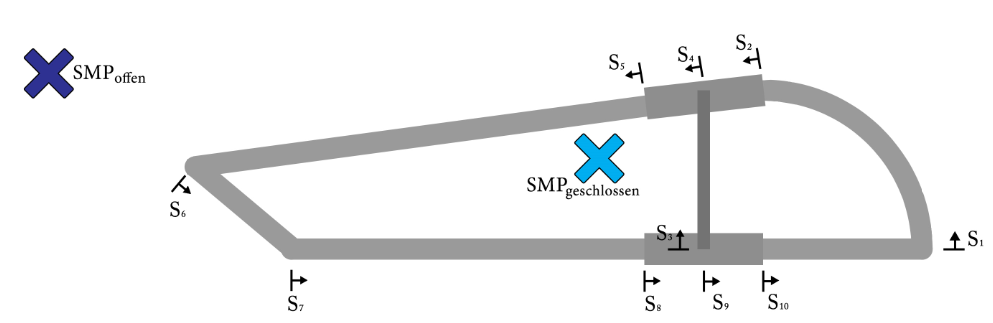
\includegraphics[width=1\textwidth]{Bilder/SMP}
	\caption{Schubmittelpunkt des geschlossenen und offenen Profils}
\end{figure}
\subsubsection{Torsion (O.S.)}
\begin{figure}[h]
	\centering
	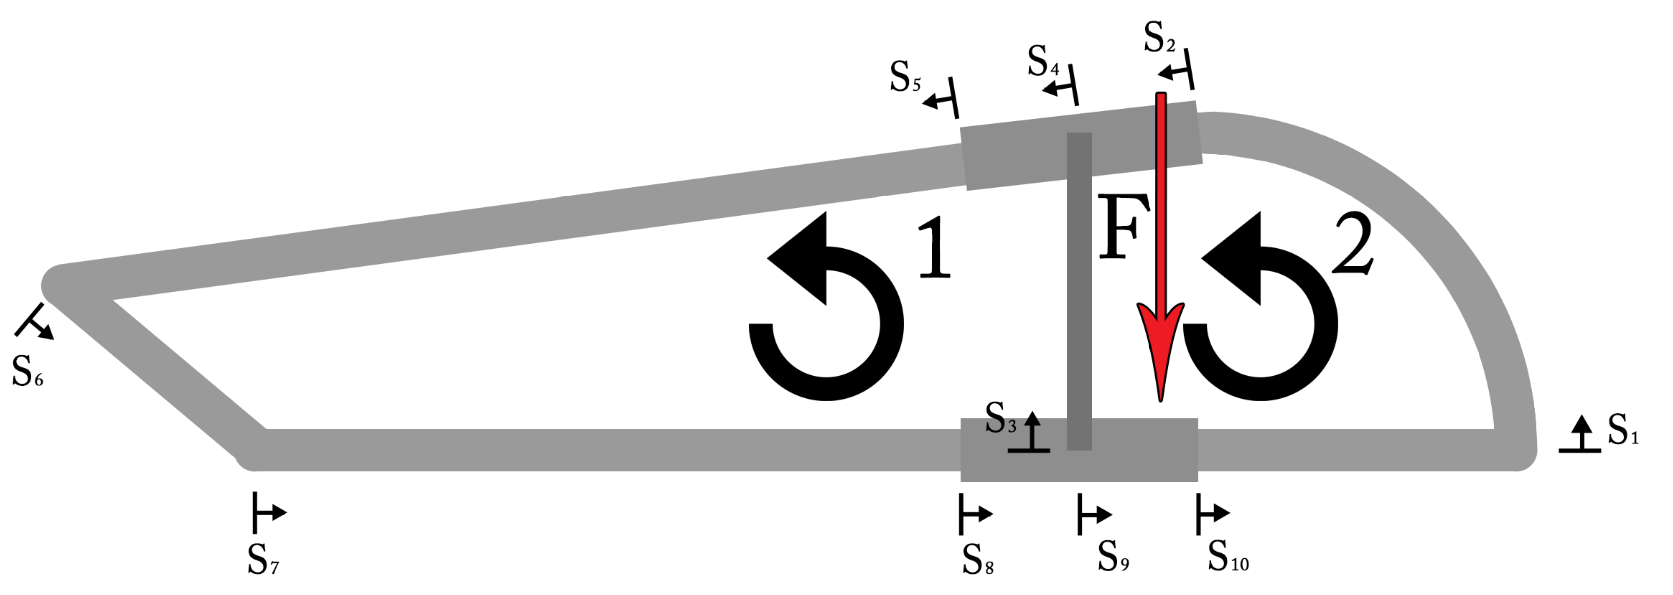
\includegraphics[width=1\textwidth]{Bilder/Torsion}
	\caption{Angreifende Kraft und positive Drehrichtung}
\end{figure}
In den bisherigen Berechnungen wurde immer davon ausgegangen, dass die Kraft im Schubmittelpunkt angreift. Durch den Versuchsaufbau ist jedoch vorgegeben, dass eine Prüflast in z-Richtung an den $l/4$-Linie aufgebracht wird. Mit dem errechneten Schubmittelpunkt lässt sich erkennen, dass ein Torsionsmoment 
\begin{equation}
	M_{xT}=(y_{l/4}-y_{0})\cdot F
\end{equation}
entsteht, das noch zusätzlichen Schubfluss und eine Verdrillung $\vartheta$ bewirkt. Genauer gesagt wird hier die St. Vernatsche Torsion behandelt, bei der zwar Verwölbung auftritt, diese aber nicht behindert wird \cite{item15}. Wieder können die konstanten Schubanteile $q_{0T,i}$ aus der Momentenäquivalenz und der Verdrillung bestimmt werden. Wobei zu beachten ist, dass der Drillwinkel hier nicht mehr wie bei der reinen Biegung null ist, aber über die Verträglichkeitsbedingung weiterhin gelten muss
\begin{equation}
	\vartheta_{1}=\vartheta_{2}=\vartheta.
\end{equation}
Da die bisherigen Anteile des Schubflusses definitionsgemäß weder Verdrillung verursachen, noch bezüglich des Schubmittelpunkts ein Moment kompensieren, fallen sie aus den Gleichungen raus. Es bleiben nur noch die Konstanten $q_{0T,i}$ übrig. Damit ergeben sich die vereinfachten Formeln für die Verdrillung und die Momentenäqivalenz:
\begin{equation}\label{verdrillung}
	\vartheta_{i} = \frac{1}{2A_{0i}G}(q_{0T,i}\oint\frac{1}{t(s)}ds-q_{0T,i\pm1}\int\frac{1}{t(s)}ds)
\end{equation}
\begin{equation}
		M_{xT}=2\sum q_{0T,i}\cdot A_{0i}
\end{equation}
Für eine maximale Prüflast von $F=500\mathrm{N}$ die der Flügel aushalten muss, erhält man
$$
	q_{0T,1}=-1,45\mathrm{N/mm}
$$
$$
	q_{0T,2}=-1,51\mathrm{N/mm}.
$$
Setzt man nun diese Werte in Gleichung (\ref{verdrillung}) erhält man für beide Zellen einen Drillwinkel von
$$
	\vartheta =-0,00195 ^\circ.
$$

\subsubsection{Schubspannung (O.S.)}
Das Ziel dieser Berechnung war nicht nur den Schubmittelpunkt und die Verdrillung zu bestimmen, sondern hauptsächlich die Schubspannung in der Haut zu erhalten, um diese auslegen zu können. Da die Hautdicke auf dem gesamten Umfang konstant bleiben soll, ist an dieser Stelle nur die maximale Schubspannung für alle Bereiche der Haut $\tau_{max}$, die sich einfach aus Gleichung (\ref{tau}) ermitteln lässt, interessant. Die Dicke $t$ ist jedoch nicht einfach aus den gesamten Rechnungen rausziehbar, weil es auch Anteile, wie zum Beispiel den Holm, gibt, die von $t$ unabhängig sind. Deswegen wird iterativ vorgegangen, wobei zuerst mit einer zufällig gewählten Dicke die Rechenschritte durchgeführt werden, in dem in diesem Kapitel gezeigten Fall mit $t=0,2\mathrm{mm}$. Am Ende der Berechnung wird aus den maximalen Schubfluss die minimale Dicke
\begin{equation}
	t_{min} = \frac{q_{max}}{R_{\tau}}.
\end{equation} 
bestimmt. Die Festigkeit bei reiner Schubbelastung $R_{\tau} = 166,67\mathrm{N/mm^2}$ wurde mittels ELamX bestimmt. Diese Dicke kann jedoch nicht als einfach so als Ergebnis genommen werden, da sich der Schubfluss mit variabler Dicke mit verändert. Die Rechnung muss mit dem neuen Wert erneut durchgeführt werden. Somit nähert man sich Schritt für Schritt dem Idealwert, bei dem die vorliegende Dicke der minimalen Dicke entspricht.

Nach einigen Iterationen bildet sich der Wert $t = 0,03\mathrm{mm}$ als Grenzwert heraus. Da dies ungefähr 0,4 Lagen bei einer Dicke $0,0783\mathrm{mm}$ des $\pm45^\circ$-Gewebes entspricht, muss für die Fertigung des Flügels auf eine ganzzahlige Lagenanzahl aufgerundet werden. Hier wurde eine Dicke von 
\begin{equation}
	t = 0,1566 \mathrm{mm}
\end{equation}
gewählt, was $2$ Lagen entspricht. Dies macht einen symmetrischen Aufbau der Haut möglich und gewährleistet die beste Beulsteifigkeit. Außerdem ist eine ausreichende Sicherheit in Folge der getroffenen Vereinfachungen gewährleistet.

Mit dieser Dicke verändern sich die Werte des endgültigen Flügels im Vergleich zu den bisher in diesem Kapitel mit $t=0,2\mathrm{mm}$ durchgeführten Berechnungen. Der Schubmittelpunkt verschiebt sich minimal zu
$$
	y_{M_{g}}=69,29\mathrm{mm}
$$
$$
	z_{M_{g}}=-20,27\mathrm{mm}.
$$
Auch der Drillwinkel vergrößert sich leicht durch die gesenkte dünnere Haut Steifigkeit zu
$$
	\vartheta =-0,0024 ^\circ.
$$
Aus den Verläufen der Schubflüsse, wie sie in Abbildung \ref{fig:S1}-\ref{fig:S10} zu sehen, erkennt man, dass die betragsmäßig maximale Schubspannung am Endpunkt des Bereichs 8 auftritt.
$$
	|\tau_{max}|=\tau(s_8=14)=42,35\mathrm{N/mm^2}\leq R_{\tau}
$$
Im Steg (Bereich 3) tritt zwar ein deutlich höherer Schubfluss auf, jedoch ergibt sich durch die ebenfalls deutlich höhere Dicke eine geringere Spannung.








\newpage
\section{CAD-Modell (H.K.)}
Auf Basis der dimensionierten Haut und des Holms soll nun ein CAD-Modell des Flügels erstellt werden. Zur Konstruktion wird das CAD-Programm Solid Edge in der Studentenversion verwendet. Als Grundlage dient eine gegebene unvollständig bemaßte technische Zeichnung der Profilkontur, aus der exakt entnommen werden kann, dass das Profil ohne die Hochauftriebselemente oder Querruder von einem Rechteck der Kantenlängen $ 172mm $, diese entspricht der Profiltiefe, und $ 37,5mm $ gerade umschlossen wird. Aus den bekannten Längenangangaben kann der Maßstab der gedruckten Zeichnung zu $ 1:1,039 $ berechnet werden. Markante Punkte entlang der Kontur können in der Zeichnung vermessen werden und mithilfe des Maßstabs auf Punkte im CAD-Modell umgerechnet werden. Im CAD-Programm werden Tangentenbögen von Punkt zu Punkt gelegt, um die Kontur hinreichend glatt anzunähern. Die verwendeten Punkte werden durch die im Anhang befindliche technische Zeichnung der Profilkontur illustriert.\\

\subsection{Konstruktion der Gurte}
\label{GurtKonstrukt}
\noindent In den Bereichen oberhalb und unterhalb des Holms soll die Haut nicht in Sandwich-Bauweise ausgeführt sein. Für die Auslegung des Holms wurde davon ausgegangen, dass eine Dicke des Verbundmaterials der Haut von $ 0,75mm $ ausreichend ist, die nach Gleichung ~\ref{gurtlagen} 9 Lagen des Interglas 90070 Gewebes entspricht. Die genauere Auslegung der Haut hat gezeigt, dass nur zwei Lagen des Gewebes notwendig sind. Der entstehende Freiraum $t_{frei}= 0,75mm-2\cdot 0,078mm=0,594mm $ zwischen der Haut und den weiter innen liegenden Gurten kann bei der Fertigung mit Harz aufgefüllt werden.\\
\noindent Der zu Beginn des Abschnitts ~\ref{GurtDim} dimensionierte Holm mit rechteckigen Gurtquerschnitten, $ b=28mm $ und $ h_{a}=36mm $, wird nun so auf die Kontur des Profils gelegt, dass die Überdeckung der Gurte mit der umgebenden Haut möglichst gering ausfällt. Dann wird die Höhe $ h_{a} $ an den örtlichen inneren Abstand der oberen und unteren Haut auf $\tilde{h_{a}}=35,8mm $ angepasst. Der rechteckige Querschnitt der Gurte wird mithilfe eines Offsets von $ {h}=1,941mm $ der Hautkrümmung angepasst. Diese Anpassungsmaßnahmen senken das Flächenträgheitsmoment leicht. Das resultierende Flächenträgheitsmoment $ \tilde{I_{x}} $ lässt sich aufgrund der komplexen Querschnittsgeometrie der Gurte nur mit dem CAD-Programm exakt bestimmen. 
\begin{figure}[h]
	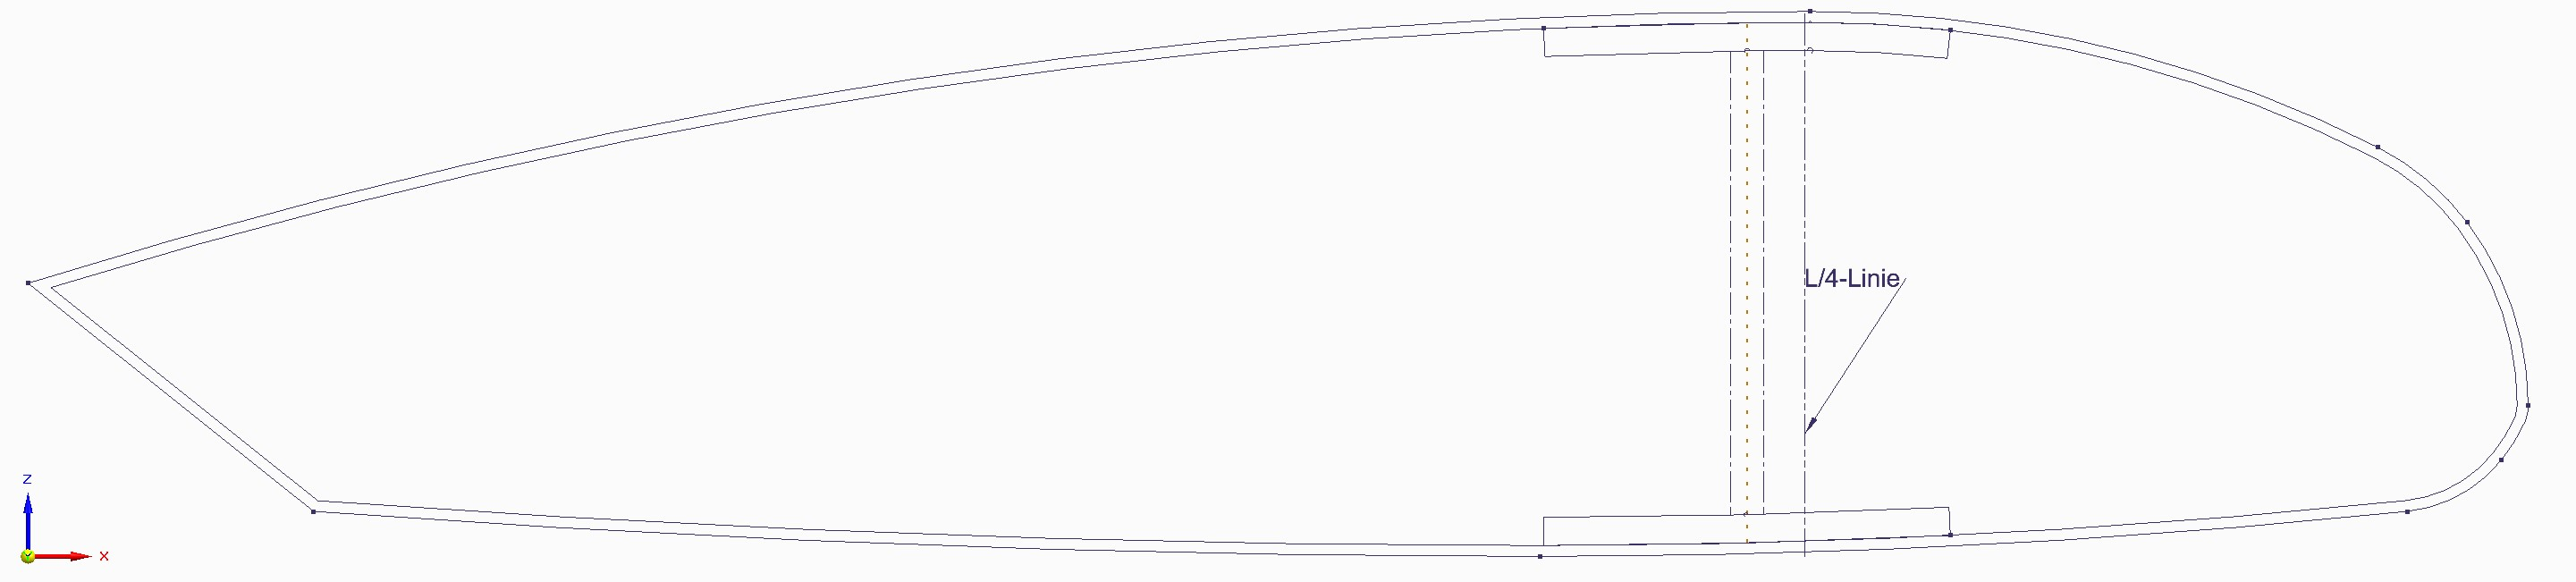
\includegraphics[width=1.0\textwidth]{Bilder/Kontur.jpg}
	\caption{Haut und Gurte nach dem ersten Schritt der Konstruktion}
	\label{fig: Kontur}
\end{figure} 
Der Vergleich mit dem erforderlichen Flächenträgheitsmoment zeigt, dass die angepasste Geometrie der Gurte die Steifigkeitsbedingung (vgl. Beziehung ~\ref{IVergleich}) erfüllt. Die Haut konstanter Dicke und die Gurte im ersten Schritt der Konstruktion werden durch Abbildung ~\ref{fig: Kontur} veranschaulicht. Zusätzlich zeigt die Abbildung die ungefähre Lage der L/4-Linie. Diese wurde mithilfe einer vorhandenen Hilfsansicht der Tragfläche inklusive der Hinterkantenklappen und des Vorflügels, beide im eingefahrenen Zustand, ermittelt. In der Hilfsansicht wird die abgebildete Länge des mittleren auszulegenden Teils der Tragfläche gemessen. Der Maßstab der ausgedruckten Hilfsansicht bezüglich des Modellmaßstabes wird zu 1:2,529 berechnet. Diese Kenntnis ermöglicht die Berechnung des Abstandes der L/4-Linie zur Vorderkante der Haupttragfläche, der $ 42,4mm $ beträgt und besonders für die Berechnung der Torsion ausschlaggebend ist.\\

\subsection{Konstruktion des Stegs}
\noindent Im nächsten Schritt werden die beiden Stegseiten und der in der Mitte liegende Schaum konstruiert. Im CAD-Programm erfolgt dies mithilfe von nur einer Skizze, die der Extrusion der Einzelteile zugrunde liegt.So kann sichergestellt werden, dass in jeder Komponente der Bezug auf die angrenzenden Gurte und die Krümmung der Seitenkanten gewahrt bleibt. Die Konstruktionen des Steges und des Schaumes erfordern auch die Berücksichtigung der verschieden belegten Unterteilungen des Steges. Während der innere Teil des Stegs, am inneren Holmstummel-Ende beginnend und $ 23mm $ in $y$-Richtung über die Aufnahme der Querkraftbolzen an Punkt C hinaus gehend, gemäß der Dimensionierung mithilfe des Laminatrechners mit 24 Lagen aufgeteilt zu jeweils zwölf Lagen auf beiden Seiten des Schaums belegt wird, soll der gesamte äußere Teil mit nur insgesamt vier Lagen gleichmäßig verteilt belegt werden. Es bietet sich an, die vier Lagen des äußeren Bereichs über die gesamte Holmlänge zu erstrecken. Die 20 verstärkenden Lagen enden $ 23mm $ hinter Punkt C in einem sanften Übergang mit einer Länge von $ 30mm $. Der dünn belegte Teil wird durch einen $ 2mm $ breiten Schaumkern vor dem Beulen geschützt, der zum dicken belegten Teil hin entsprechend schmaler wird. Das innere Holmstummel-Ende wird auf eine Länge von $ l_{0}=30mm $ im Abstand vom Mittelpunkt des Lagers A abgeschätzt. Abbildung ~\ref{fig: Steg} veranschaulicht den prinzipiellen Aufbau qualitativ. Eine technische Zeichnung im Anhang illustriert die Konstruktion von Gurten und Steg. Sie gibt außerdem Aufschluss über die wichtigsten Maße und stellt die unterschiedlichen Wandstärken des Schaumkerns und des Faserverbundanteils im Steg für die verschiedene Bereiche im Querschnitt grafisch dar.

\begin{figure}[h]
	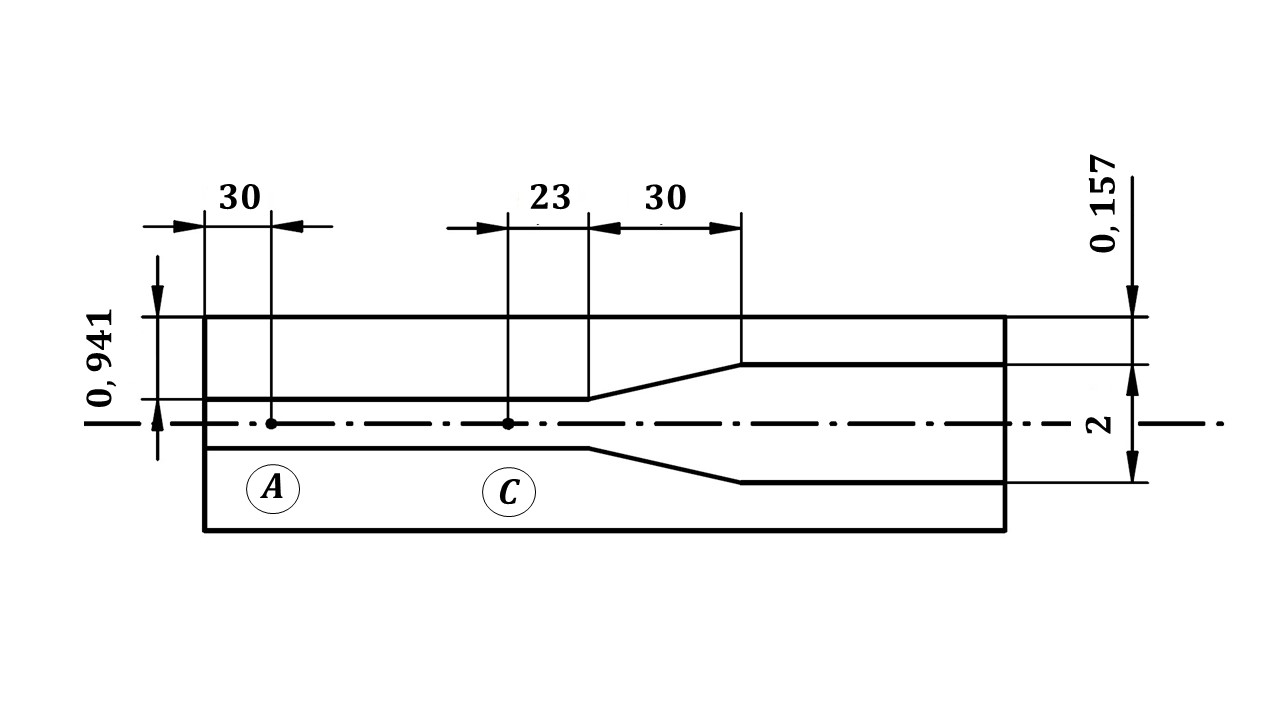
\includegraphics[width=1.0\textwidth]{Bilder/StegPrinzip.jpg}
	\caption{Prinzipskizze der Sandwichstruktur im Steg}
	\label{fig: Steg}
\end{figure}


\subsection{Konstruktion der Haut und der Rippen}
Um die Haut vor Beulerscheinungen zu schützen, soll ein Schaumkern zwischen die innere und äußere Hautschicht gelegt werden. Der Beulberechnung ist zu entnehmen, dass mit einem $ 3mm $ dicken Kern ausreichende Sicherheit gegen Beulen gegeben ist. Ein Schaumkern dieser Stärke ist darüber hinaus gut handhabbar und kann mithilfe eines heißen Drahtes einfach und kostengünstig aus einem Styrodurklotz ausgeschnitten werden. Um die Höhe $ h_{a} $ der Gurte möglichst nicht durch die Haut einzuschränken, soll der Schaumkern zu den Gurten hin über $ 5mm $ in einem sanften Übergang auslaufen, sodass nur das Laminat über und unter den Gurten hergeführt werden muss. Abbildung ~\ref{fig: Hautuebergang} veranschaulicht die prinzipielle Gestaltung der Haut im Bereich des oberen Gurtes, der grau dargestellt ist. \\

\noindent Der Freiraum zwischen Gurten, den Steglagen und der inneren Hautlage kann nun für die Vorder- und Hinterseite des Steges umrandet werden. Die darauf basierende Skizze ist die Grundlage der Konstruktion der zweigeteilten Wurzel- und Endrippe. Die Rippen werden in ihrer Dimensionierung als gegeben angenommen, eine Auslegung erfolgt im Rahmen dieser Projektarbeit nicht. Ein Belastungstest der Tragfläche würde in der Realität durch eine an der Endrippe befestigte Last erfolgen. Damit die Last angeschlagen werden kann, müssen zwei Bohrungen in der Endrippe vorgesehen werden, deren Abstand durch das gegebene Bauteil Endscheibe bestimmt wird. Zur einfachen Montage der Last werden zwei Gewindehülsen konstruiert, die in die Bohrungen eingefügt werden.

\begin{figure}[h]
	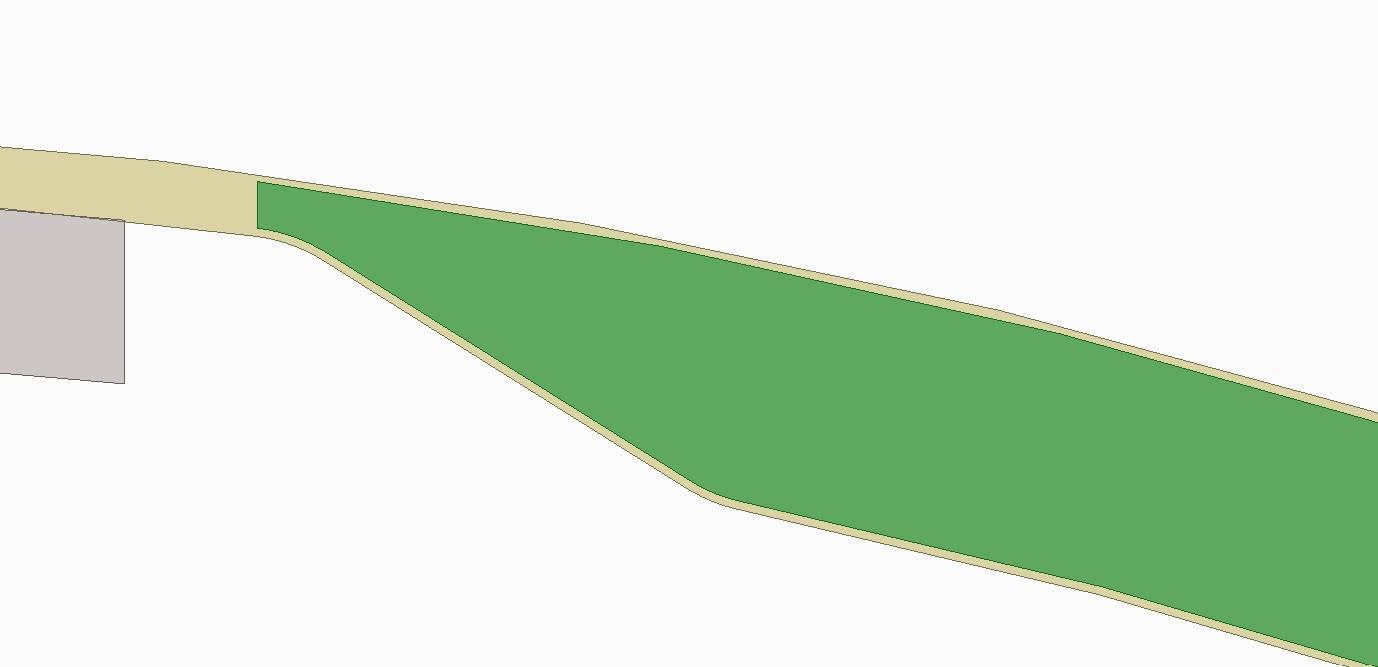
\includegraphics[width=1.0\textwidth]{Bilder/Hautuebergang.jpg}
	\caption{Hautsandwich am Übergang zum Gurt}
	\label{fig: Hautuebergang}
\end{figure}

\subsection{Holzkonstruktion an der Aufnahme der Hauptbolzen}
Die Kraftaufnahme der  als Fest- und Loslager modellierten Punkte A und B erfolgt durch zwei Hauptbolzen, die im Flugzeug die Tragflächen miteinander verbinden. In diesem Fall werden die Lagerkräfte von maximal $ 5085N $ an den Teststand übertragen. Damit bei der Krafteinleitung in den Holm Spannungsspitzen vermieden werden, soll die Auflagefläche der Bolzen vergrößert werden. Dies geschieht, indem eine Holzkonstruktion für Vorder- und Rückseite des Holms erstellt wird, die der Kontur der Gurte angepasst ist und Bohrungen für die Bolzen enthält. Diese Klötze werden auf ihrer jeweiligen Stegseite mit den Gurten und dem Steg verklebt. Da der Abstand der Bohrungen mit $ 76mm $ gering ist, wird ein längerer Holzklotz für beide Bohrungen konstruiert. Aussparungen an den Seiten und zwischen den Bohrungen sollen das Gewicht der Klötze reduzieren. Zum Schutz der Hauptbolzen werden zwei Messinghülsen konstruiert und in die Bohrungen eingefügt. So kann verhindert werden, dass die gefetteten Bolzen bei Montage und Demontage Späne aus dem Steg lösen oder sich verkanten. Die Messinghülsen weisen eine Wandstärke von $ 0,5mm $ und einen Innendurchmesser von $ 8mm $ auf. In der Fertigung kann auf kostengünstige Messingrohre zurückgegriffen werden. Die Konstruktion wird durch Abbildung ~\ref{fig: Klotz} veranschaulicht. Eine technische Zeichnung des vorderen Holzklotzes mit Angaben zu den Hauptabmessungen befindet sich im Anhang.
\begin{figure}[h]
	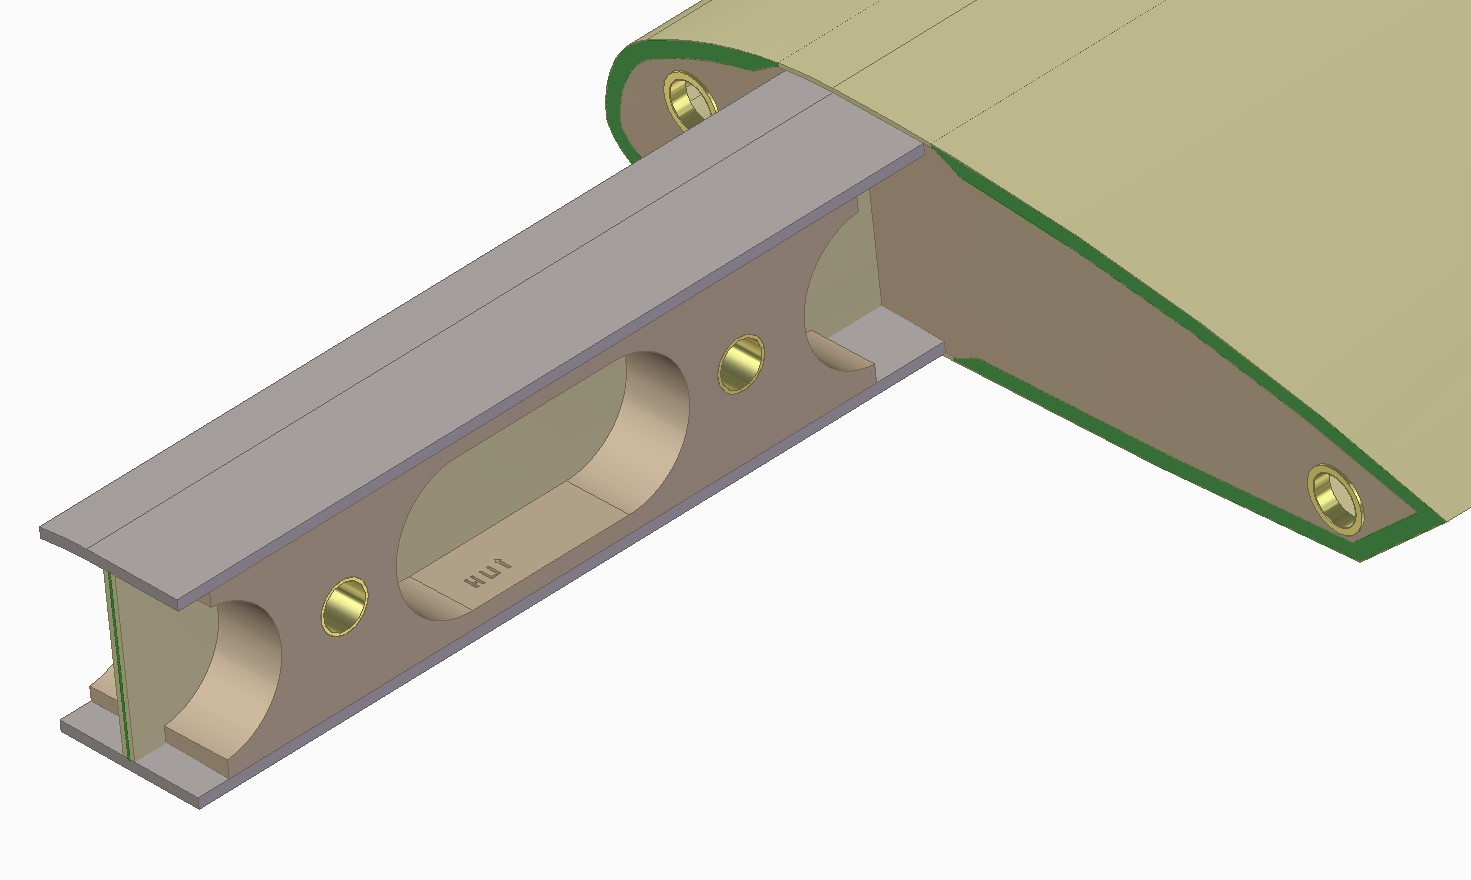
\includegraphics[width=1.0\textwidth]{Bilder/Klotz.jpg}
	\caption{Holzklötze und Hülsen}
	\label{fig: Klotz}
\end{figure}

\subsection{Querkraftbolzen und Montage auf dem Teststand}
Die Prüfung, ob die gesamte Auslegung der Tragfläche den Bestimmungen der Aufgabenstellung gerecht wird, erfolgt anhand einer FEM-Berechnung, anstelle der tatsächlichen Fertigung des Flügels und des Bruchtests. Dennoch kann mithilfe gegebener Zeichnungen der Teststandelemente geprüft werden, ob die konstruierte Tragfläche in der Realität auf dem Teststand montierbar wäre. Der Abstand der Hauptbolzen zueinander wurde bereits in der frühen Modellierung des Holms als Biegebalken berücksichtigt. Für die Positionierung der Bohrungen und Hülsen der Querkraftbolzen wird der Abstand zwischen den Langlöchern und der Aussparung für den Holm in der Montageplatte gemessen. An der gegenüberliegenden Wurzelrippe können so die Bohrungen festgelegt werden. Bei Verwendung der Maße aus der gegebenen technischen Zeichnung der Montageplatte, fällt auf, dass das Langloch zur Aufnahme des hinteren Querkraftbolzens für diese Konstruktion ungeeignet ist. Es liegt außerhalb des Bereichs der Wurzelrippe. Dies wird auf die Anordnung des Holms in der Tragfläche zurückgeführt, die die Position der Flügelkontur bezüglich der Montageplatte festlegt. Sie kann nachträglich nicht ohne größere Änderungen des Holmquerschnitts und eine damit verbundene Neuauslegung verändert werden. Abbildung \ref{fig: SeiteRichtig} des Anhangs veranschaulicht die ursprüngliche Lage des hinteren Langlochs. Um eine grundsätzlich neue Dimensionierung aller Komponenten zu vermeiden, wurde die Position des Langlochs angepasst. Da die Querkraftbolzen einen großen Abstand zueinander aufweisen (vgl. Abb. \ref{fig: Klotz}), müssen zur Aufnahme der Torsionsmomente nur kleine Kräfte übertragen werden. Die Radien der Langlöcher in der Montageplatte begrenzen den Durchmesser der Querkraftbolzen auf $ 8,5mm $. Auch für die Querkraftbolzen werden Hülsen konstruiert, die die Wurzelrippe schützen und die Montage erleichtern. Sie sind in \ref{fig: Klotz} ebenfalls dargestellt.\\

\noindent Alle Komponenten der Tragfläche und ihre Positionen sind im Anhang auf einer Explosionszeichnung ersichtlich. Eine Grafik des gesamten CAD-Modells und der Bauteile des Teststandes ist ebenfalls im Anhang enthalten (vgl. Abb. \ref{fig:AufbauGesamt}).Abbildung \ref{fig:MontagePlatte} zeigt die auf der Montageplatte positionierte Tragfläche unter Verwendung des angepassten Langlochs.

\newpage
\section{Zusammenfassung}
\subsection{Die Berechnungen im Überblick (H.K.)}
Im Folgenden werden die Ergebnisse der Auslegungsschritte und Berechnungen zusammengefasst und die wichtigsten Aspekte herausgestellt.\\

\noindent Die gesamte Auslegung folgte übergeordneten Zielsetzungen, die das mechanische Verhalten bei quasistatischer Belastung an der Endrippe vorgeben. Bei einer Prüfkraft von $ F_{pruef}=100N $ darf sich die Flügelspitze um höchstens $ w(100N)=22mm $ absenken. Um diese Bedingung sicher zu erfüllen wurde ein Sicherheitsfaktor von $ j=1,1 $ festgelegt, der die zulässige Absenkung auf $ w_{j=1,1}(100N)=20mm $ verringert. Bei einer Prüfkraft von $ F_{pruef}=500N $ darf die Tragfläche nicht versagen und Beulerscheinungen dürfen nicht auftreten. Zusätzlich sollte ein Hauptaugenmerk auf das möglichst geringe Gewicht der Konstruktion gerichtet sein.\\

\noindent Der Auslegung des Holms ging die \textit{Modellierung als Biegebalken} voraus, der mit der schubstarren Balkentheorie nach Bernoulli berechnet wurde. Zur Modellierung wurden die Hauptbolzen Lager interpretiert, die Querkraftbolzen und die Prüfkraft als äußere Lasten. Vorgegebene Längenangaben des Teststandes und der Tragfläche bestimmen die Maße der einzelnen Bereiche. Für jeden Bereich wurden die Differentialgleichungen des Biegebalkens aufgestellt und gelöst. Die zentralen Ergebnisse sind die Kenntnisse der Schnittkraft- und -momentenverläufe, sowie die erforderliche Biegesteifigkeit von $ EI_{x}=962,552Nm^{2} $ zur Einhaltung der maximalen Absenkung $ w_{j=1,1}(100N) $. Zur Einhaltung der Anforderungen an die Festigkeit sind die Querkräfte $ Q_{1}(500N)=5085,5N $ in Bereich 1, $ Q_{2}(500N)=0N $ in Bereich 2 und $ Q_{3}(500N)=-500N $ in Bereich 3 relevant.\\

\noindent Die \textit{Holmgurte} nehmen, entsprechend der Schubfelträgertheorie, das Biegemoment auf und sind damit Hauptbestandteil der Auslegung zur Einhaltung des Steifigkeitskriteriums. Um das erforderliche Flächenträgheitsmoment der Rechteckquerschnitte, das sich aus der Biegesteifigkeit $ EI_{x} $ und dem aus der Mischungsregel bestimmbaren E-Modul in Fadenrichtung $ E_{11}=31580MPa $ berechnen lässt, bei einer möglichst kleinen und damit gewichtsoptimierten Querschnittsfläche zu erreichen, wurden die Gurte in z-Richtung möglichst weit auseinander gelegt und möglichst breit in x-Richtung gestaltet. Die resultierende Gurtdicke wird mit $ n=9 $ Lagen des annähernd unidirektionalen Gewebes Interglas 92145 erreicht und beträgt damit $ \tilde{h}=1,941mm $. Die Anpassung der rechteckigen Gurtquerschnitte an die gekrümmte Profilkontur der Tragfläche verringert das Flächenträgheitsmoment leicht, dennoch ist das dadurch entstandene $ \tilde{I_{x}}>I_{min} $ und die in den Randfasern resultierende Spannung an der Stelle der maximalen Biegebeanspruchung weniger als halb so groß, wie die zulässige Spannung des unidirektionalen Handlaminats.\\

\noindent Der \textit{Holmsteg} wird durch drei Kraftflüsse beansprucht. Durch die stoffschlüssige Verbindung von Gurten und Steg wird die Längsdehnung $ \epsilon_{Gurt} $ dem Steg aufgeprägt und führt zu einem Normalkraftfluss $ n_{\epsilon} $ parallel zu den Gurten. Aufgrund der Absenkung des Holms entstehen Druckkräfte, die eine zu den Gurten senkrechten Kraftfluss $ n_{A} $ erzeugen. Zusätzlich wirkt ein Schubfluss $ q_{s} $. Zur Vorauslegung wurde der Glasfaserverbund durch allgemeine Dimensionierungskennwerte charakterisiert, bezüglich der Steifigkeitseigenschaften mit $ K_{E\#} $ und mit $ K_{\sigma d} $ für die Festigkeitseigenschaften. Mithilfe der VDI 2013 konnten auf diese Weise die Lagenanzahlen zu $ n=20 $ für die Bereiche 1 und 2 und $ n=2 $ für den Bereich 3 bestimmt werden.\\

\noindent Der Tatsache, dass die Auslegung des Holmstegs nach dieser Richtlinie nur überschlägig erfolgt, wurde in der detaillierteren Dimensionierung mit der \textit{CLT} Rechnung getragen. Diese berücksichtigt die gegebenen Materialkennwerte des Laminats. Die aus der Balkenanalyse und Schubflussberechnung hervorgehenden Beanspruchungen, sowie die Lagenanzahlen der Vorauslegung wurden als Grundlage für das Festigkeitskriterium nach Puck verwendet. Mithilfe des Laminatrechners ließen sich die Lagenanzahlen und Beanspruchungen variieren und Sicherheiten gegen Faser- und Zwischenfaserbruch bestimmen. Die Analyse hat gezeigt, dass die Lagenanzahlen erhöht werden mussten, auf $ n=24 $ in den Bereichen $I$ und $II$, sowie $ n=4 $ im Bereich 3.\\

\noindent Um die \textit{Sicherheit gegen Beulen} für den Holm zu prüfen, wurden anschließend der auf Druck beanspruchte Gurt und der Steg mithilfe der Berechnungsmethoden nach Hertel analysiert. Für den Druckgurt konnte unter Verwendung des E-Moduls und der Gurtdicke die Sicherheit gegen Beulen zu $ j_{Gurt}=1,08 $ bestimmt werden. Der Steg wurde bereichsweise mit den jeweils vorliegenden Biege- und Schubbeanspruchungen untersucht. Die Bereiche 1 und 2 sind mit Sicherheiten von $ j_{1}=1,148 $, bzw. $ j_{2}=1,59 $ schon ohne die Verwendung eines Schaumkerns sicher gegen Beulen. Für den Bereich 3 ist eine Sandwichkonstruktion zur Gewährleistung der Beulsicherheit notwendig. Ein $ 2mm $ starker Schaumkern wurde gewählt, um die Fertigung zu vereinfachen. Damit ergibt sich eine Beulsicherheit von $ j_{3}=6,88 $ im Bereich 3 und eine zusätzliche Sicherheit für die Bereiche 1 und 2.\\

\noindent Die \textit{Klebeverbindungen} zwischen dem Steg und den Gurten werden durch das Aufbringen von Mumpe hergestellt. Mit der gegebenen Schubfestigkeit $ \tau_{Mumpe}=10MPa $ wird eine Klebebreite von $ l=15,9mm $ in den Bereichen 1 und 2 benötigt, für den schwächer beanspruchten Bereich 3 reichen $ l=1,62mm $. Bei einer Prüfkraft von $ F_{pruef}=500N $ wird gemäß der grundlegenden Annahme $ F_{Q}=F_{pruef} $ eine ebenso große Kraft über die Wurzelrippe abgesetzt. Eine schmale Holzleiste mit einer Breite von $ 1,56mm $ kann auf jeder Seite des Stegs die Klebefläche zwischen Wurzelrippe und Steg bereitstellen.\\

\noindent Als Verbindung der Tragfläche zum Teststand sind zwei \textit{Hauptbolzen} und zwei Querkraftbolzen vorgesehen, deren Durchmesser bereits durch die Bohrungen im Teststand festgelegt ist. Beide Hauptbolzen werden bei einer Prüfkraft von $ F_{pruef}=500N $durch eine $ 5085,5N $ beansprucht. Unter Berücksichtigung der Bolzenlänge wurde eine Mindeststreckgrenze des Bolzenwerkstoffs von $ R_{e}=360,8MPa $ ermittelt. Als Werkstoff für alle Bolzen wurde daraufhin S620Q gewählt. Diese Wahl gewährleistet auch, dass die Querkraftbolzen mit einem Durchmesser von $ d=8mm $ sicher ausgelegt sind.\\

\noindent Die im Allgemeinen außerhalb des Schubmittelpunkts der Tragfläche angreifende Belastung, führt zu einem Torsionsmoment und einer Biegebelastung des Flügels. Letztere wird durch den Holm aufgenommen, der unter dieser Annahme bereits dimensioniert wurde, ersteres muss durch die Flügelschale aufgenommen werden und darf hier nicht zu Beulerscheinungen führen. Zur Bestimmung des Schubflusses in der Schale, wurde die Profilkontur durch zehn Abschnitte angenähert und der Schaum der Sandwichkonstruktion vernachlässigt. Für die erste Berechnung wurde die Hautdicke zu $ t=0,2mm=konst. $ angenommen. Bezüglich der vordersten Kante und der speziell definierten Koordinatenrichtungen des angenäherten Profils liegt der Schwerpunkt bei $ y_{0}=78,53mm $ und $ z_{0}=-15,39mm $. Über die Flächenträgheits-, Deviations- und statischen Momente wurde die Lage des Schubmittelpunkts im Falle des offenen Profils lokalisiert, der bei $ y_{M}=207,60mm $ und $ z_{M}=-41,35mm $ und damit, wie erwartet, außerhalb des Profils liegt. Die Kontur wurde geschlossen und über die Momentenäquivalenz die Lage des Schubmittelpunktes zu $ y_{Mg}=76,78mm $, $ z_{Mg}=-21,56mm $ berechnet. Für den enstandenen Zweizeller wurde unter Annahme gleicher Verwindung beider Zellen der Drillwinkel bei einer Belastung von $ F_{pruef}=500N $ im l/4-Punkt zu $ \varphi=-1,87^{\circ} $ ermittelt. Darüber hinaus konnte mit den Kenntnissen auftretender Schubflüsse die maximale Schubspannung ermittelt werden. Zur Dimensionierung der Hautstärke wurde die Berechnung der Schubflüsse für mehrere Hautstärken $ t $ vorgenommen. Die so bestimmten maximalen Schubflüsse wurden mit den zugehörigen Lagenaufbauten in den Laminatrechner $ eLamX^{2} $ eingegeben, um die Sicherheiten gegen Faser- und Zwischenfaserbruch zu ermitteln. $ n=2 $ Lagen ermöglichen eine Sandwichkonstruktion und sichern die Auslegung gegenüber den Vereinfachungen ab. Daraus ergab sich ein Drillwinkel für die neue Dicke von $ \varphi(500N)=-2,32^{\circ} $.\\

\noindent Die Auslegung nach Handbuchmethoden wurde durch die \textit{Beulabschätzung der Flügelschale} abgeschlossen. Dazu wurde der gefährdetsten Profilabschnitt betrachtet, dessen Krümmung vernachlässigt wurde, um die Sicherheit zu erhöhen und um die Rechnung zu vereinfachen. Weiterhin wurde mit der größten auftretenden Schubspannung gerechnet, obwohl diese nicht im betrachteten Bereich vorliegt. Bei Verwendung eines 3mm dicken Schaumkerns ergibt sich eine Sicherheit gegen Beulen von $ j=1,09 $. Die Wahl der Schaumdicke ist durch die einfache Fertigbarkeit begründet. Die großzügige Auslegung wirkt sich wegen der sehr geringen Dichte des Styrodurs nur unwesentlich auf die Massenbilanz aus. 


\subsection{Die Konstruktion und FEM-Analyse im Überblick (H.K.)}
Als \textit{Grundlage der FEM-Analyse} und zur Veranschaulichung der vorangegangenen Auslegung nach Handbuchmethoden, wurde ein Modell der Tragfläche im CAD-Programm erstellt. Es berücksichtigt alle bisherigen geometrischen Größen. Desweiteren wurden zusätzliche Bauteile und Details erstellt. Für die Sandwichkonstruktion der Flügelschale wurde eine Lösung gefunden, bei der der Schaumkern die beulgefährdeten Bereiche schützt, im Bereich der Gurte jedoch ausläuft, um die Höhe $ h_{a} $ des Holms nicht weiter einzuschränken. Es wurden Wurzel- und Endrippe konstruiert, in denen Bohrungen zur Aufnahme der Querkraftbolzen und zur Verschraubung der Endplatte vorgesehen sind. Messinghülsen wurden für die Bohrungen der Bolzen erstellt, um die betreffenden Bereiche zu schützen und die Montage zu erleichtern. Auch die Holzklötze, die die Auflagefläche der Hauptbolzen am Steg vergrößern, wurden konstruiert. Alle Bauteile wurden zum Schluss im CAD-Programm zusammengebaut. Die jeweiligen Dichten wurden den Komponenten zugeordnet und ermöglichten eine Massenabschätzung des Tragflügels zu $ m_{ges}=0,366kg $. \\

\noindent Der im CAD-Programm zusammengebaute Tragflügel wurde zur \textit{FEM-Analyse in Abaqus} importiert. Die Analyse dünnwandiger Bauteile wird durch die Verwendung von Schalenmodellen erleichtert, sodass der Volumenkörper im ersten Schritt in Flächen umgewandelt wurde. Die Materialkennwerte für Styrodur und GFK wurden in das Programm integriert und das Laminat zusammengestellt. Anschließend wurde den einzelnen Flächen die Dicke des zugehörigen Bauteils, bei GFK-Teilen die jeweilige Lagenanzahl zugeordnet. Lager A und B wurden als feste Einspannung modelliert, die Querkraftbolzen und Prüfkraft als äußere Lasten, letztere mit Angriffspunkt im l/4-Punkt. Die Analyse hat zeigt, dass sich die Flügelspitze bei einer Prüfkraft von $ F_{pruef}=100N $ um $ w(100N)=17,34mm $ absenkt. Dieses Ergebnis bestätigt die Einhaltung der Anforderung an die Steifigkeit die eine Absenkung von $ w_{zul}=20mm $ erlaubt. Um die Einhaltung der Festigkeitsanforderungen zu prüfen, wurde ein Prüfkraft von 500N eingestellt. Spannungsspitzen ergaben sich im Bereich der Hauptbolzen, die jedoch durch die nicht modellierten Holzklötze gemildert würden. Genauere Aussagen zur Ertragbarkeit der Belastungen, lieferte die Analyse der größten aufgetretenen Dehnungen im Faserkoordinatensystem, die als für alle Lagen gleich groß angenommen wurden. Die Dehnungen konnten in $elamX^{2}$ übertragen werden, um auf diese Weise die Sicherheiten gegen Faser- und Zwischenfaserbruch einer Komponente an einer kritischen Stelle zu ermitteln. Bei einer Prüfkraft von $ F_{pruef}=500N $ ergaben sich die kleinsten Sicherheiten gegen Zfb im Steg zu $ j_{min}=2,32 $, in der Haut zu $ j_{min}=2,785 $, am oberen Gurt zu $ j_{min}=2,332 $ und am unteren Gurt zu $ j_{min} =1,312$. Es wird vermutet, dass diese, gegenüber der beabsichtigten Auslegung, großen Sicherheiten auf die konservativen Annahmen der einzelnen Auslegungsschritte zurückzuführen sind. Die gegenseitige Stützung der Komponenten untereinander, die in der Auslegung nach Handbuchmethoden nicht berücksichtigt werden konnten, wird so deutlich.\\

\noindent Mithilfe des FEM-Programms wurde auch eine \textit{Beulanalyse} durchgeführt. Da der Holmstummel nicht genau genug modelliert werden konnte, wurde vereinfachend eine Einspannung an den Querkraftbolzen angenommen. Nahe dieser Einspannung tritt das Beulen am ehesten auf. Der Beulfaktor entspricht dem Sicherheitsfaktor bzgl. einer Beulform. Selbst bei $ F_{pruef}=1000N $ beträgt er noch $ 1,0253 $, damit wird die Konstruktion als sicher gegen Beulen im beabsichtigten Bereich der Prüfkraft angenommen.





\subsection{Gewichtsnormalisiertes Festigkeitskriterium (O.S.)}
Um eine Vergleichbarkeit zwischen verschiedenen Flügeln zu schaffen wird die gewichtsnormalisierten Festigkeit
\begin{equation}
	P=\frac{m_{\mathrm{Belastung,max}}}{m_{\mathrm{Fluegel}}}
\end{equation}
definiert. Es wird also die Gewichtskraft als Masse $m_{\mathrm{Belastung,max}}$, die der Flügel im Testaufbau maximal aushält, ins Verhältnis mit der Flügelmasse $m_{\mathrm{Fluegel}}$ gesetzt. Auch wenn das Ziel war, einen möglichst leichten Flügel, der den in der Aufgabenstellung formulierten Anforderungen entspricht, zu konstruieren, wird somit berücksichtigt, dass mehr Material zwar eine höhere Masse mit sich bringt, aber er wahrscheinlich auch größere Lasten aushalten kann. Üblicher Weise würde man die Bruchlast im Teststand ermitteln, aber auf Grund der COVID-19 Pandemie ist es uns nicht möglich den Flügel zu bauen, geschweige denn zu testen.\\
	
\noindent Eine Möglichkeit wäre es $500$ Newton als Bruchlast anzunehmen, da wir im Rahmen der Projektarbeit nachgewiesen haben, dass unsere Konstruktion dies aushält. Da jedoch immer eher vorsichtige Annahmen getroffen und die errechneten Werte dann meist noch aufgerundet wurden, wäre die gewichtsnormalisierten Festigkeit weit unter dem voraussichtlich im Teststand ermittelten Wert. Somit wäre der Aussagewert sehr gering.
Eine bessere Möglichkeit bietet hier das FE-Modell. Dies ist zwar auch nicht perfekt, da zum einen die Einspannung auf Grund der Holzblöcke nicht perfekt realistisch modelliert werden kann. Die kritischste Stelle liegt nach Überlegungen und durch ABAQUS bestätigt am Ansatz des Holmstummels, also dem Flügelende, dass am Rumpf anliegt, bzw. an der Stelle, wo der GFK im Steg dicker wird. Diese Stellen liegen weit genug von der Einspannung entfernt, sodass die Werte als plausibel angenommen werden können. Zum anderen ist durch die Studentenversion von ABAQUS der Idealisierungsgrad auf $1000$ Knoten und somit auch die Genauigkeit der Ergebnisse beschränkt. Trotzdem ist dies mit den zur Verfügung stehenden Mitteln der beste Ansatz um die Bruchlast zu ermitteln, da hier als Einziges der Flügel als Ganzes modelliert wird.\\

\noindent Da nicht bekannt ist, in welchem Bereich das Material zuerst versagt, wird in Gurt, Steg und Schale jeweils der Ort der höchsten Belastung einzeln betrachtet. Da nur ein einheitlich Wert für die Spannung der Elemente gegeben wird, diese in Realität aber nicht über alle Schichten konstant ist, wird die Dehnung betrachtet, da sie für alle identisch ist. Wird nun die Dehnung in die beiden Achsenrichtungen und der Schubwinkel in $elamX^{2}$ eingegeben, erhält man sofort die Sicherheit gegen den Bruch. Die Ergebnisse sind in Abbildung \ref{sicher-steg} bis \ref{sicher-gurt} zu erkennen, wobei es zwei verschieden Werte für den Holm gibt, da er auf der einen Seiten auf Druck und auf der anderen auf Zug belastet wird. Der untere Gurt hat demnach die geringste Sicherheit von $1,31$. Da die Belastung im Flügel linear mit der anliegenden Kraft steigen, lässt sich der Faktor direkt auf die aufgebrachte Last von $500\mathrm{N}$ übertragen. Somit ergibt sich eine Bruchlast von 650N oder mit einer Erdbeschleunigung von $9,81\frac{\mathrm{m}}{\mathrm{s^2}}$
$$m_{\mathrm{Belastung,max}} = 66,26\mathrm{kg}. $$ Eine erneute FEM-Berechnung mit der gesteigerten Kraft liefert neue Dehnungen, die im Gurt wie erwartet eine Sicherheit von ungefähr $1$ ergeben. Da der kleinste Beulfaktor deutlich höher als diese Sicherheit war, kommt es auch nicht bei der erhöhten Last zum Beulen.
Für das Gewichtsnormalisiertes Festigkeitskriterium ergibt sich nun also mit $m_{\mathrm{Fluegel}}$ aus der Massenabschätzung ungefähr ein Wert von
$$P = 181,04.$$
\subsection{Diskussion der Ergebnisse}
\subsection{Ausblick auf Optimierungen der Berechnungen (H.G.)}
Da für die Auslegung viele Annahmen und Vereinfachungen getroffen wurden, lassen sich einige Optimierungsmöglichkeiten für das Projekt nennen.\\
\noindent
Zunächst ließe sich die Dicke der Gurte über der Holmlänge als nicht konstant annehmen um zusätlich das Gewicht zu verringern. Da dies jedoch schwer bis nicht analytisch zu lösen wäre und einen signifikanten Mehraufwand für eine relativ kleine Gewichtsänderung mit sich gebracht hätte, wurde in dieser Arbeit davon abgesehen.\\
\noindent
Die Wurzelrippe wurde mit einer definierten Dicke als gegeben angesehen. Hier wäre ebenfalls eine Möglichkeit, um evtl. Gewicht einzusparen und die Absenkung zusätzlich zu verringern. Da dies jedoch zusätzliche Einarbeitung in die Holztechnik und deutlich mehr Zeitaufwand mit sich bringen würde, wurde hier davon abgesehen.\\
\noindent
Die Berechnung des FKV wurde mit mittels der Mischungsregel durchgeführt. In alternativer Literatur wurde dies beispielsweise nach Puck berechnet. Dadurch könnten sich genauere Materialkennwerte ergeben, was zu einer möglichen Verringerung der GFK Schichten und somit des Gewichts führen könnte. Dies würde aber wiederum zu einer deutlich aufwändigen Rechnung führen, deren Ertrag zu gering ist, um dies zu rechtfertigen.\\
\noindent
In mehreren Berechnungen wurden schwächere Annahmen getroffen, als die Realität widerspiegelt. So wurde in der Auslegung des Holms und der Haut die Steifigkeit des Schaums nicht mit einberechnet, wodurch etwas Leichtbaupotential verschenkt wurden.\\
\noindent
Es wurde in vielen Fällen mit einer Sicherheit gerechnet. Da in den Annahmen und in den Materialkennwerten schon eine gewisse Ungenauigkeit und diese oft kleiner als in der Realität sind, können die Sicherheitswerte herabgesetzt werden, oder sogar gleich 1 gesetzt werden.\\
\noindent
Die FEM-Modellierung ist ebenfalls in vielerlei Hinsicht optimierbar. Durch die Studentenversion kann das Bauteil nicht so genau vernetzt werden, wie es für eine genau Auswertung nötig wäre. Zusätzlich sind die Holzblöcke am Holmstummel nicht modelliert worden, da dies sehr aufwändig gewesen wäre.\\
\noindent
 

\newpage
\section{FEM}
\subsection{Warum FEM? (O.S.)}
Nachdem der Flügel nun analytisch ausgelegt wurde, stellt sich die Frage, ob eine numerische Herangehensweise hier überhaupt noch sinnvoll ist. In den vorherigen Kapiteln wurde viele Vereinfachungen angenommen, um die Berechnungen mit verhältnismäßigen Aufwand zu bewältigen. Je komplexer ein Bauteil ist, desto unwirtschaftlicher wird es, dieses in seiner Fülle analytisch zu berechnen oder gar unmöglich, wenn keine geschlossenen Lösungen bekannt sind. Im Leichtbau werden diese Details benutzt, um Beiteile an de Stellen zu verstärken, wo besonders große Lasten auftreten (z.B. Rippen). Wenn diese nun für eine einfachere Berechnung wegfallen, muss das Restliche Bauteil robuster ausgelegt werden, was zu einer vermeidbaren Gewichtszunahme führt. Auch wenn es sich bei numerischen Lösungen nur um Annäherungen an den wahren Zustand handelt, kann durch einen hohen Vernetzungsgrad ein präziseres Ergebnis erzielt werden als das vereinfachte Analytische. Somit übernimmt die nummerische Berechnung auch eine Kontrollfunktion.
\subsection{Wie funktioniert FEM? (O.S.)}
\subsubsection{Schwache Lösung der Elastostatik}
Für die Berechnung der Elastostatik sind die Gleichgewichtsbedingung (\ref{GGB}),  Verzerrungs-Verschiebungsbedingung (\ref{VVB}) und das Stoffgesetz (\ref{SG}) auch bei der Finiten Elemente Methode (FEM) ausschlaggebend.
\begin{equation}\label{GGB}
	\underline{0} = \underline{X} + \underline{\underline{E}}^T \sigma 
\end{equation}
\begin{equation}\label{VVB}
	\underline{\epsilon} = \underline{\underline{D}} \underline{u}
\end{equation}
\begin{equation}\label{SG}
	\underline{\sigma} = \underline{\underline{E}} \underline{\epsilon}
\end{equation}
Wobei \underline{$X$} der Vektor der Volumenkräfte, \underline{\underline{$E$}} die Steifigkeitsmatrix, \underline{$\epsilon$} der Verzerrungsvektor, \underline{$u$} der Verschiebungsvektor und \underline{\underline{$D$}} die Operatormatrix ist.\\
Um einer aufwendigen Bestimmung der analytischen Lösung zu entgehen, bedient sich die FEM an dem Prinzip der \textit{schwachen Lösung}. Hierbei hat man eine Differenzialgleichung, die in dem betrachteten Gebiet gleich null ist. Für die Elastostatik kann man hierbei die Gleichgewichtsbedingung verwenden. Diese kann man mit $\delta\underline{u}$ multiplizieren und über das Gebiet integrieren, sodass man
\begin{equation}
	\int_{V}^{}\delta\underline{u}^T\underline{\underline{D}}^T\underline{\sigma}\,dV + \int_{V}^{}\delta\underline{u}^T\underline{X}\,dV = 0
\end{equation}
erhält. Umgeformt ergibt sich das zu
\begin{equation}\label{SL}
	\int_{V}^{}\delta\underline{u}^T\underline{\underline{D}}^T\underline{\underline{E}}\underline{\underline{D}}\underline{u}\,dV = \int_{O_{p}}^{}\delta\underline{u}^T\underline{p}\,dO_p + \int_{V}^{}\delta\underline{u}^T\underline{X}\,dV
\end{equation}
Wobei die Terme auf der rechten Seite den Lasten entsprechen, die auf das Volumen $V$ und die mit $p$ belastete Oberfläche $O_{p}$ wirken. Die schwer zu lösende Differenzialgleichung hat sich nun schon zu einem Integrationsproblem vereinfacht. Daraus kann die Verschiebung bestimmt werden, weswegen man dies auch die Weggrößenmethode nennt. Die Verzerrungen und Spannungen erhält man aus Nachrechnungen mit den Gleichungen (\ref{VVB}) und (\ref{SG}) berechnet werden. Diese Gleichung ist noch ganz allgemein fürs Kontinuum gültig. Im nächsten Schritt wird das Gebiet in eine finite Menge von Elementen zerteilt.
\subsubsection{Diskretisierung}
Die Werte der Verschiebung $\underline{u}$ werden nur an Aufpunkten, den sogenannten Knoten, bestimmt. Mittels einer von Laufvariable $\underline{x}$ abhängigen Formfunktion $\underline{\underline{N}}$ wird der Verlauf von einem Knoten zu seinen Nachbarn definiert, um wieder einen kontinuierlichen Verlauf zu erhalten. Hierbei muss die Formfunktion an dem Knoten, von dem sie ausgeht, den Wert $1$  und bei jedem anderen den Wert $0$ annehmen. Allgemein ergibt sich somit
\begin{equation}
	\underline{u}(\underline{x})=\underline{\underline{N}}(\underline{x})\underline{u}^{(e)}
\end{equation}
, wobei $\underline{u}^{(e)}$ der Vektor der Verschiebungen eines Elementes $e$ ist.
Wenn man nun diese Gleichung in die Gleichung der schwachen Lösung (\ref{SL}) einsetzt, lässt sich $\delta(\underline{u}^{(e)})^T$ aus den Integralen raus ziehen und kürzen, da es von $\underline{x}$ unabhängig sind.
\begin{equation}
	\int_{V}^{}\underline{\underline{N}}^T\underline{\underline{D}}^T\underline{\underline{E}}\underline{\underline{D}}\underline{\underline{N}}\,dV\underline{u}^{(e)} = \int_{O_{p}}^{}\underline{\underline{N}}^T\underline{p}\,dO_p + \int_{V}^{}\underline{\underline{N}}^T\underline{X}\,dV
\end{equation}
Wobei sich das linke Integral zu der Elementsteifigkeitsmatrix $\underline{\underline{K}}^{(e)}$ ergibt.
\begin{equation}
	\underline{\underline{K}}^{(e)} = \int_{V}^{}\underline{\underline{N}}^T\underline{\underline{D}}^T\underline{\underline{E}}\underline{\underline{D}}\underline{\underline{N}}\,dV
\end{equation}
Die einzelnen Elementsteifigkeitsmatrixen lassen sich zu einer Gesamtsteifigkeitsmatrix zusammenfassen, mit der dann die Lösung berechent wird. --> Beispiel einfügen?
\newpage
\section{Quellenverzeichnis}
\begin{thebibliography}{99}          
	\bibitem{item1}
	H. Hertel :
	\textit { Leichtbau:Bauelemente,Bemessungen und Konstruktionen von Flugzeugen u.a. }.
	Springer Verlag Berlin/Göttingen/Heidelberg , 1960.
	
	\bibitem{item2}
	Mises, R. V. :
	\textit { Fluglehre: Vorträge über Theorie und Berechnung der Flugzeuge in elementarer Darstellung }.
	Springer Verlag , 1936.
	
	\bibitem{item3}
	Helmut Schürmann :
	\textit { Konstruieren mit Faser-Kunststoff-Verbunden }.
	Springer Verlag , 2005.
	
	\bibitem{item4}
	Elmar Witten :
	\textit { Handbuch Faserverbundkunststoffe, Composites: Grundlagen, Verarbeitung, Anwendungen }.
	Springer Vieweg , 2014.
	





	
	
\end{thebibliography}
\newpage
\section{Abbildungsverzeichnis}
\listoffigures
\newpage
\section{Tabellenverzeichnis}
\listoftables
\newpage
\section{Anhang}
\subsection{Berechnung: Analytischen Lösung der Holm-Modellierung}
In diesem Abschnitt werden die Gleichungen \ref{eq:34}, \ref{eq:35} und \ref{eq:36} herlgeleitet:
\begin{itemize}
	\item Aus Gleichung \ref{eq:11} und \ref{eq:22} ergibt sich:
	\begin{equation}\label{eq:164}
		R_{4}=0
	\end{equation}
	\item Aus Gleichung \ref{eq:9} und \ref{eq:23} ergibt sich:
	\begin{equation}\label{eq:165}
		R_{2}=0
	\end{equation}
	\item Aus Gleichung \ref{eq:18} und \ref{eq:33} ergibt sich:
	\begin{equation}\label{eq:166}
		R_{9}=-F
	\end{equation}
	\item Aus Gleichung \ref{eq:13}, \ref{eq:18}, \ref{eq:33} und \ref{eq:166} ergibt sich:
	\begin{equation}\label{eq:167}
		R_{5}=-F_{pruef}-F_{Q}
	\end{equation}
	\item Aus Gleichung \ref{eq:19} , \ref{eq:32} und \ref{eq:166} ergibt sich:
	\begin{equation}\label{eq:168}
		R_{10}=F_{pruef}\cdot (l_{1}+l_{2}+l_{3})
	\end{equation}
	\item Aus Gleichung \ref{eq:14}, \ref{eq:19}, \ref{eq:30}, \ref{eq:166}, \ref{eq:167} und \ref{eq:168} ergibt sich:
	\begin{equation}\label{eq:169}
		R_{6}=F_{pruef}\cdot (l_{1}+l_{2}+l_{3}) + F_{Q}\cdot (l_{1}+l_{2})
	\end{equation}
	\item Aus Gleichung \ref{eq:9}, \ref{eq:14}, \ref{eq:27}, \ref{eq:167} und \ref{eq:169} ergibt sich:
	\begin{equation}\label{eq:170}
		R_{1}=F_{pruef}\cdot\frac{l_{2}+l_{3}}{l_{1}} + F_{Q}\cdot\frac{l_{2}}{l_{1}}
	\end{equation}
	\item Aus Gleichung \ref{eq:11}, \ref{eq:24} und \ref{eq:170} ergibt sich:
	\begin{equation}\label{eq:171}
		R_{3}=-\frac{1}{6}\cdot F_{pruef}\cdot (l_{2}+l_{3})\cdot l_{1} - \frac{1}{6}\cdot F_{Q}\cdot l_{2}\cdot l_{1}
	\end{equation}
	\item Aus Gleichung \ref{eq:10}, \ref{eq:15}, \ref{eq:26}, \ref{eq:167}, \ref{eq:169}, \ref{eq:170} und \ref{eq:171} ergibt sich:
	\begin{equation}\label{eq:172}
		R_{7}=F_{pruef}\cdot \Bigl[-\frac{1}{2} l_{1}^{2}-\frac{2}{3} l_{1}l{2}-\frac{2}{3} l_{1}l{3}\Bigr] + F_{Q}\cdot \Bigl[-\frac{1}{2} l_{1}^{2}-\frac{2}{3} l_{1}l{2}\Bigr]
	\end{equation}
	\item Aus Gleichung \ref{eq:16}, \ref{eq:25}, \ref{eq:167}, \ref{eq:169} und \ref{eq:172} ergibt sich:
	\begin{equation}\label{eq:173}
		R_{8}=F_{pruef}\cdot \Bigl[\frac{1}{6} l_{1}^{3}+\frac{1}{6} l_{1}^{2}l{2}+\frac{1}{6} l_{1}^{2}l{3}\Bigr] + F_{Q}\cdot \Bigl[\frac{1}{6} l_{1}^{3}+\frac{1}{6} l_{1}^{2}l{2}\Bigr]
	\end{equation}
	\item Aus Gleichung \ref{eq:15}, \ref{eq:20}, \ref{eq:29}, \ref{eq:166}, \ref{eq:167}, \ref{eq:168}, \ref{eq:169} und \ref{eq:172} ergibt sich:
	\begin{equation}\label{eq:174}
		R_{11}=F_{pruef}\cdot \Bigl[-\frac{1}{2} l_{1}^{2}-\frac{2}{3} l_{1}l{2}-\frac{2}{3} l_{1}l{3}\Bigr] + F_{Q}\cdot \Bigl[\frac{1}{2} l_{1}^{2}+\frac{1}{3} l_{1}l{2}\Bigr]
	\end{equation}
	\item Aus Gleichung \ref{eq:16}, \ref{eq:21}, \ref{eq:28}, \ref{eq:166}, \ref{eq:167}, \ref{eq:168}, \ref{eq:169}, \ref{eq:172}, \ref{eq:173} und \ref{eq:174} ergibt sich:
	\begin{equation}\label{eq:175}
		R_{12}=F_{pruef}\cdot \Bigl[\frac{1}{6} l_{1}^{3}+\frac{1}{6} l_{1}^{2}l{2}+\frac{1}{6} l_{1}^{2}l{3}\Bigr] + F_{Q}\cdot \Bigl[-\frac{1}{6} l_{2}^{3}-\frac{1}{3} l_{1}^{2}l{2}-\frac{1}{2} l_{2}^{2}l{1}\Bigr]
	\end{equation}
	\item Nun können die Gleichungen \ref{eq:166}, \ref{eq:167}, und \ref{eq:170} in folgende Gleichung eingesetzt werden, sodass sich Gleichung \ref{eq:34} ergibt:
	\begin{equation}
		Q(y,F_{pruef},F_{Q},EI_{x})=\left\{\begin{array}{ll}
			-R_{1}&,y\epsilon (0,l_{1})\\
			-R_{5}&,y\epsilon (l_{1}+l_{2})\\
			-R_{9}&,y\epsilon (l_{1}+l_{2}+l_{3})
		\end{array}\right.
	\end{equation}
	\item Nun können die Gleichungen \ref{eq:165}, \ref{eq:166}, \ref{eq:167}, \ref{eq:168}, \ref{eq:169} und \ref{eq:170} in folgende Gleichung eingesetzt werden, sodass sich Gleichung \ref{eq:35} ergibt:
	\begin{equation}
		M(y,F_{pruef},F_{Q},EI_{x})=\left\{\begin{array}{ll}
			-R_{1}\cdot y - R_{2}&,y\epsilon (0,l_{1})\\
			-R_{5}\cdot y - R_{6}&,y\epsilon (l_{1}+l_{2})\\
			-R_{9}\cdot y - R_{10}&,y\epsilon (l_{1}+l_{2}+l_{3})
		\end{array}\right.
	\end{equation}
	\item Nun können die Gleichungen  \ref{eq:164}, \ref{eq:165}, \ref{eq:166}, \ref{eq:167}, \ref{eq:168}, \ref{eq:169}, \ref{eq:170},  \ref{eq:171},  \ref{eq:172},  \ref{eq:172},  \ref{eq:174} und  \ref{eq:175} in folgende Gleichung eingesetzt werden, sodass sich Gleichung \ref{eq:36} ergibt:
	\begin{equation}
		w(y,F_{pruef},F_{Q},EI_{x})=\left\{\begin{array}{ll}
			\frac{1}{EI}\cdot\Bigl(\frac{R_{1}\cdot y^{3}}{6}+\frac{R_{2}\cdot y^{2}}{2}+R_{3}\cdot y +R_{4}\Bigr)&,y\epsilon (0,l_{1})\\
			\frac{1}{EI}\cdot\Bigl(\frac{R_{5}\cdot y^{3}}{6}+\frac{R_{6}\cdot y^{2}}{2}+R_{7}\cdot y +R_{8}\Bigr)&,y\epsilon (l_{1}+l_{2})\\
			\frac{1}{EI}\cdot\Bigl(\frac{R_{9}\cdot y^{3}}{6}+\frac{R_{10}\cdot y^{2}}{2}+R_{11}\cdot y +R_{12}\Bigr)&,y\epsilon (l_{1}+l_{2}+l_{3})
		\end{array}\right.
	\end{equation}
\end{itemize}
\newpage
\subsection{Abbildungen}
\begin{figure}[h]
	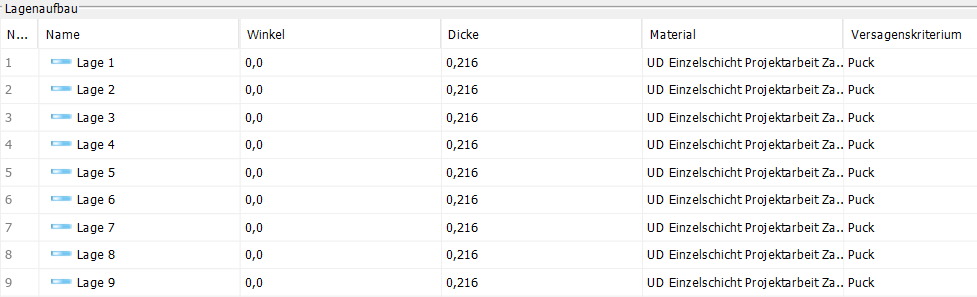
\includegraphics[width=1.0\textwidth]{Bilder/Lagenaufbau Holmgurte.png}
	\caption{Lagenaufbau Holmgurte}
	\label{fig:Lagenaufbau Holmgurte}
\end{figure}
\begin{figure}[h]
	\includegraphics[width=1.0\textwidth]{Bilder/Lagenaufbau Steg dünn.png}
	\caption{Lagenaufbau Steg Bereich $III$}
	\label{fig:Lagenaufbau Steg dünn}
\end{figure}
\begin{figure}[h]
	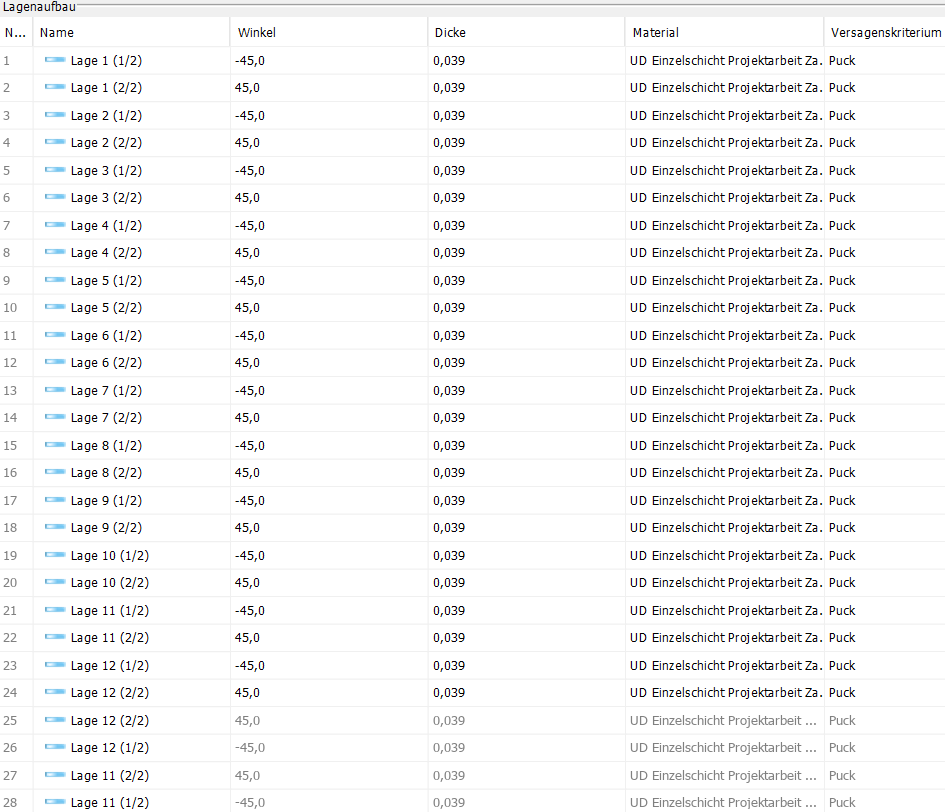
\includegraphics[width=1.0\textwidth]{Bilder/Lagenaufbau Steg dick.png}
	\caption{Lagenaufbau Steg Bereich $I$\&$II$}
	\label{fig:Lagenaufbau Steg dick}
\end{figure}
\begin{figure}[h]
	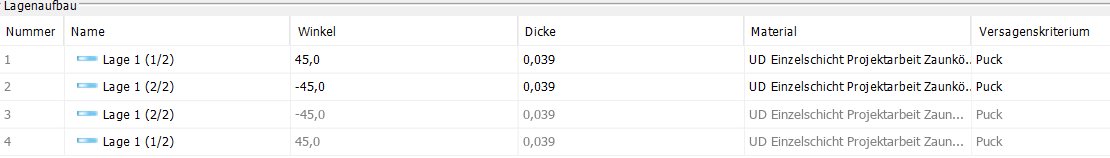
\includegraphics[width=1.0\textwidth]{Bilder/Lagenaufbau Haut.png}
	\caption{Lagenaufbau Flügelschale}
	\label{fig:Lagenaufbau Haut}
\end{figure}
\begin{figure}[h]
	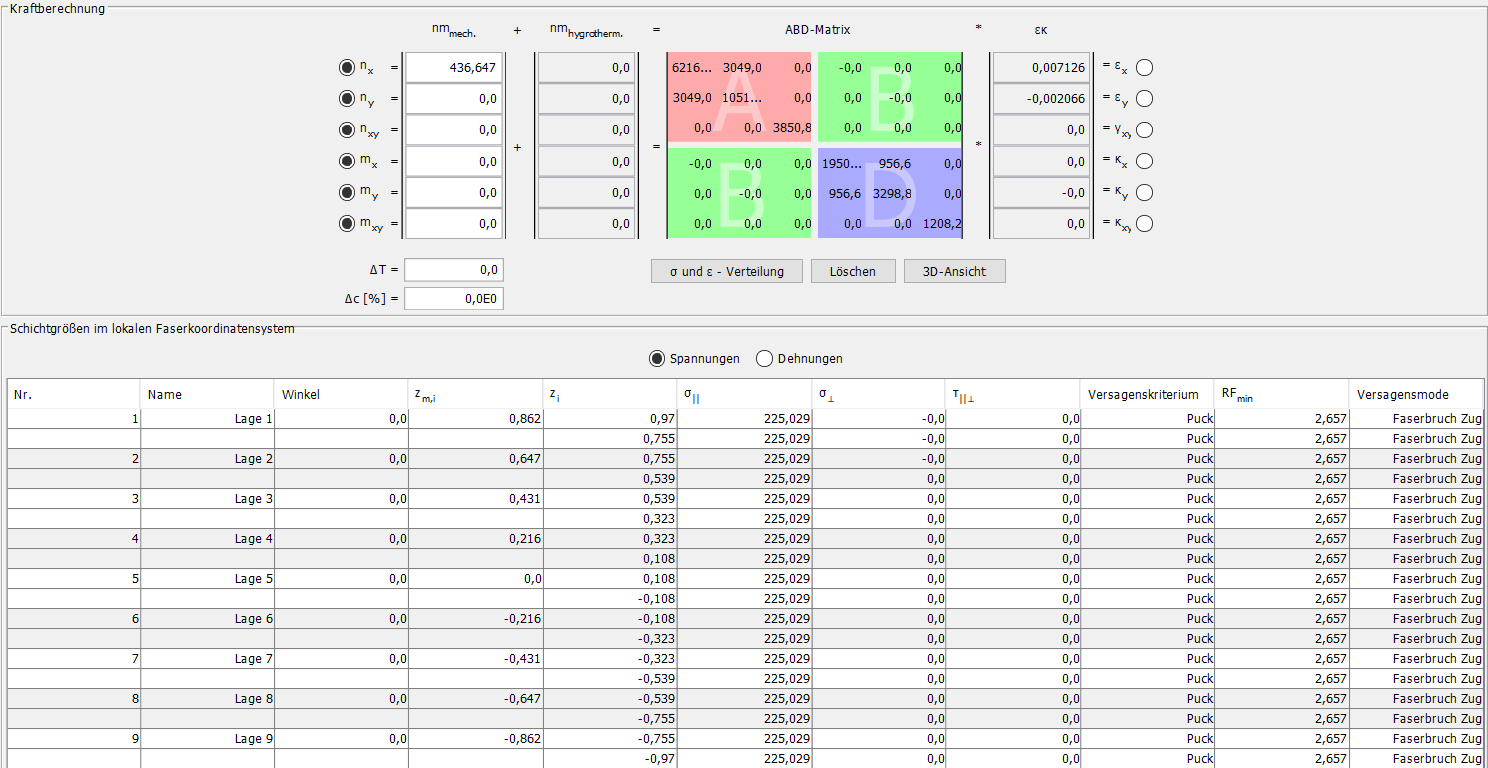
\includegraphics[width=1.0\textwidth]{Bilder/Berechnung Holmgurte.png}
	\caption{Berechnung Holmgurte}
	\label{fig:Berechnung Holmgurte}
\end{figure}
\begin{figure}[h]
	\includegraphics[width=1.0\textwidth]{Bilder/Berechnung Steg dünn.png}
	\caption{Berechnung Steg Bereich $III$}
	\label{fig:Berechnung Steg dünn}
\end{figure}
\begin{figure}[h]
	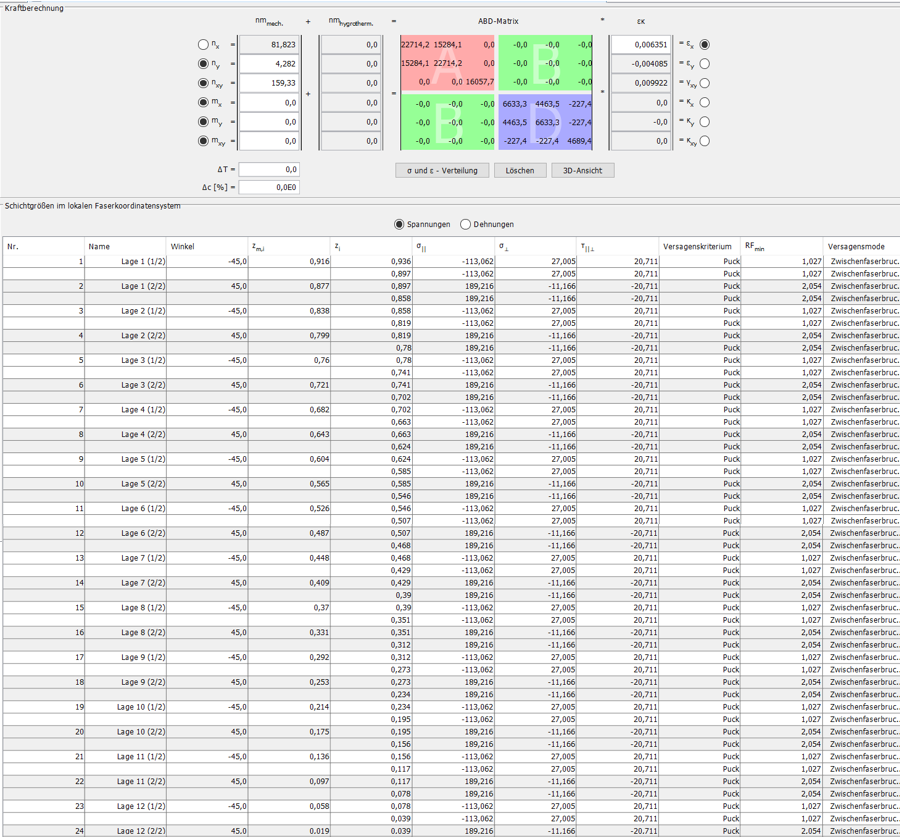
\includegraphics[width=1.0\textwidth]{Bilder/Berechnung Steg dick.png}
	\caption{Berechnung Steg Bereich $I$\&$II$}
	\label{fig:Berechnung Steg dick}
\end{figure}
\begin{figure}[h]
	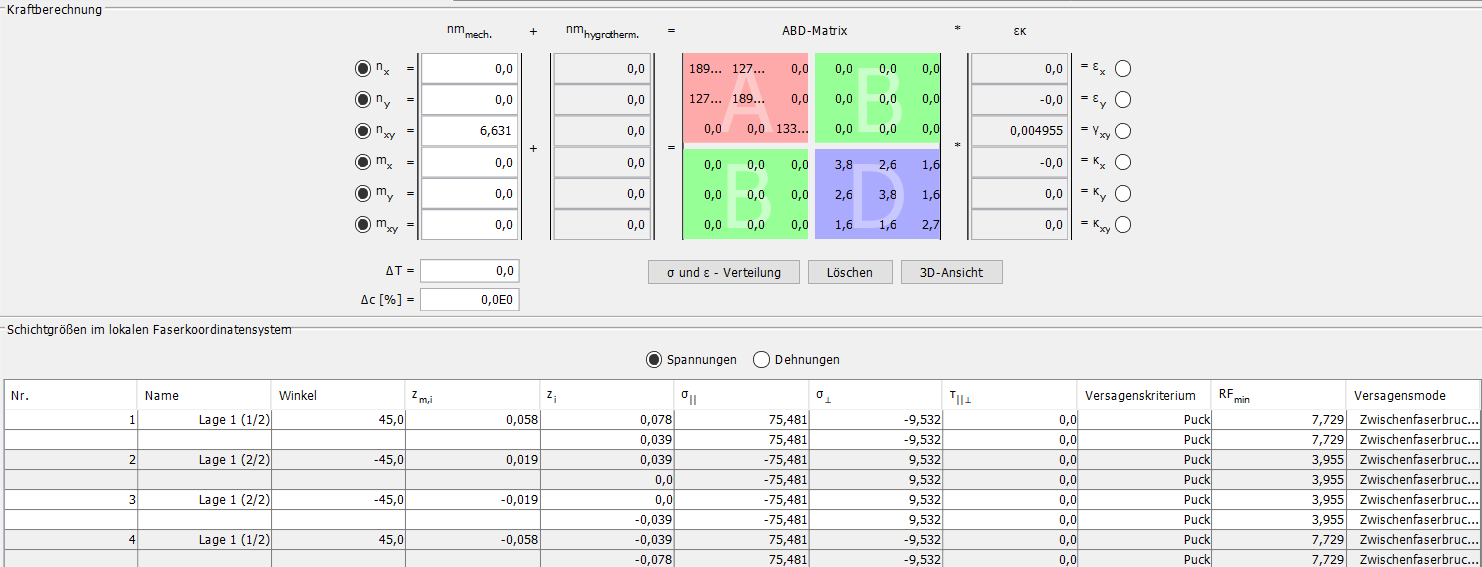
\includegraphics[width=1.0\textwidth]{Bilder/Berechnung Haut.png}
	\caption{Berechnung Flügelschale}
	\label{fig:Berechnung Haut}
\end{figure}
\begin{figure}[h]
	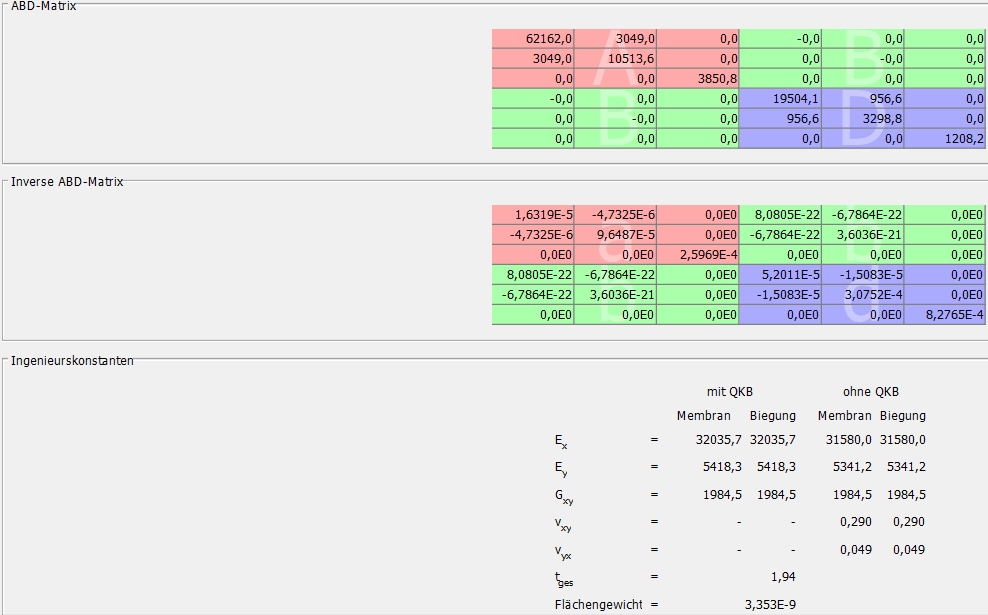
\includegraphics[width=1.0\textwidth]{Bilder/Konstanten Holmgurte.png}
	\caption{Ingenieurskonstanten Holmgurte}
	\label{fig:Ingenieurskonstanten Holmgurte}
\end{figure}
\begin{figure}[h]
	\includegraphics[width=1.0\textwidth]{Bilder/Konstanten Steg dünn.png}
	\caption{BerechnIngenieurskonstantenung Steg Bereich $III$}
	\label{fig:Ingenieurskonstanten Steg dünn}
\end{figure}
\begin{figure}[h]
	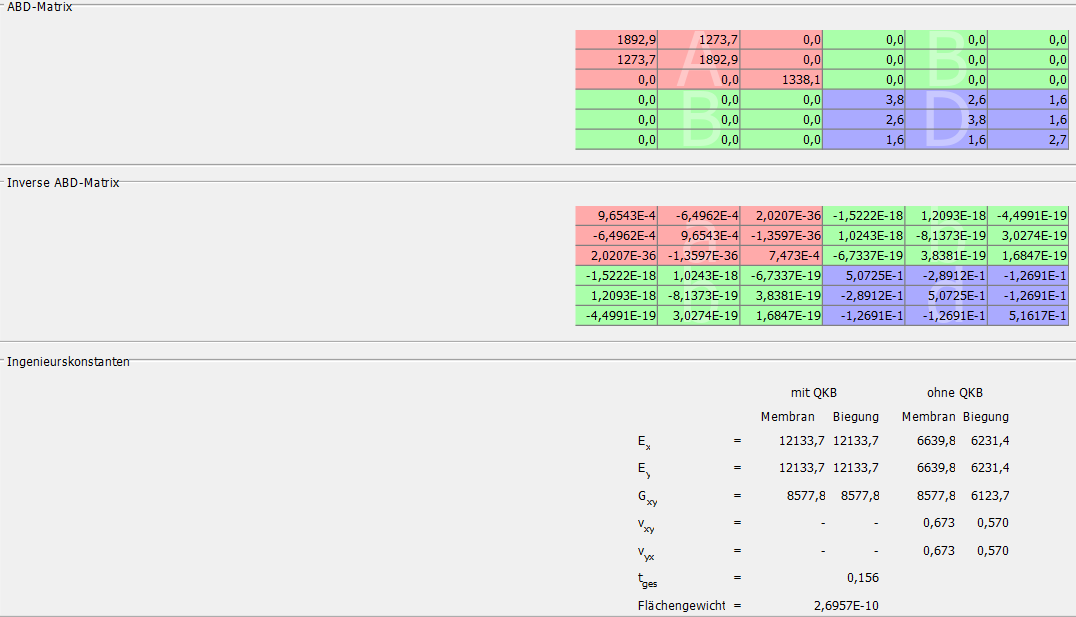
\includegraphics[width=1.0\textwidth]{Bilder/Konstanten Haut.png}
	\caption{Ingenieurskonstanten Flügelschale}
	\label{fig:Ingenieurskonstanten Haut}
\end{figure}
\begin{figure}[h]
	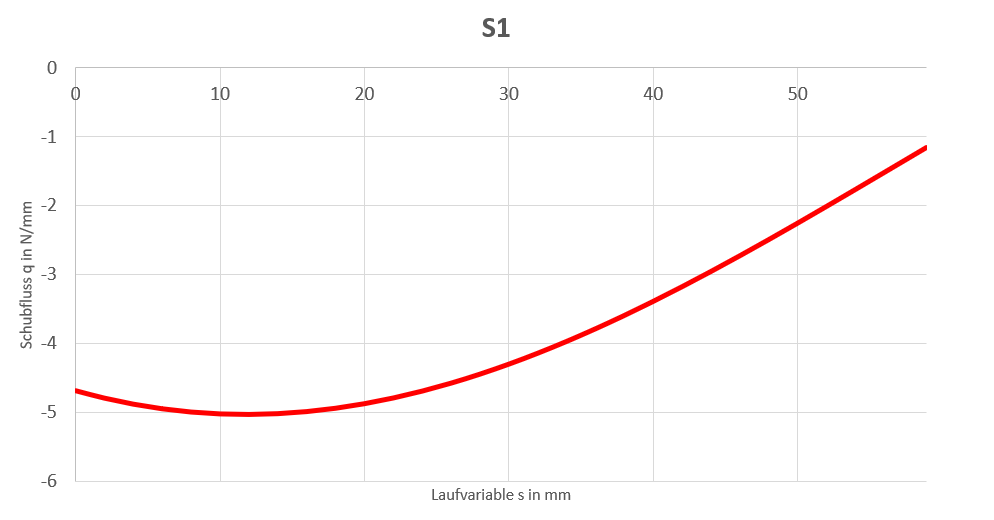
\includegraphics[width=1.0\textwidth]{Bilder/S1.png}
	\caption{Schubfluss Bereich $I$}
	\label{fig:S1}
\end{figure}
\begin{figure}[h]
	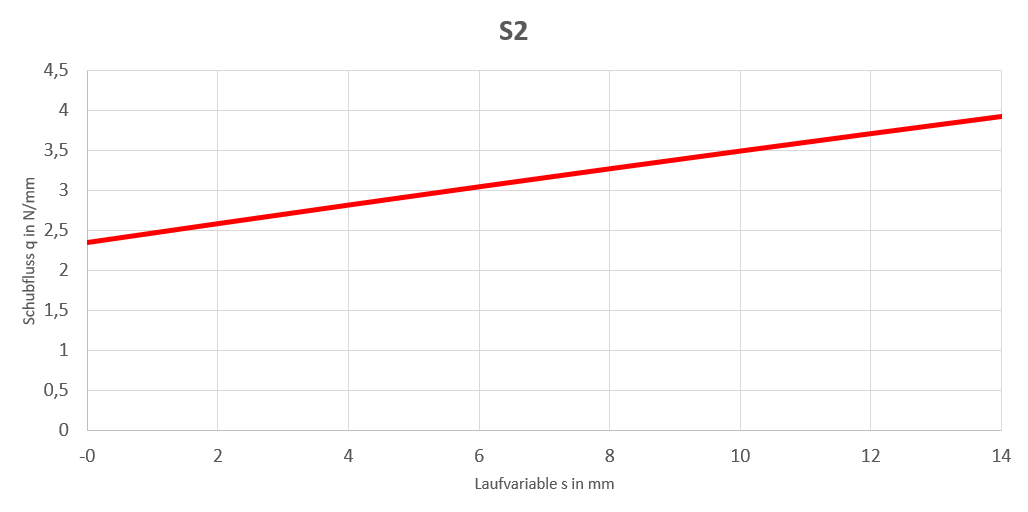
\includegraphics[width=1.0\textwidth]{Bilder/S2.png}
	\caption{Schubfluss Bereich $II$}
	\label{fig:S2}
\end{figure}
\begin{figure}[h]
	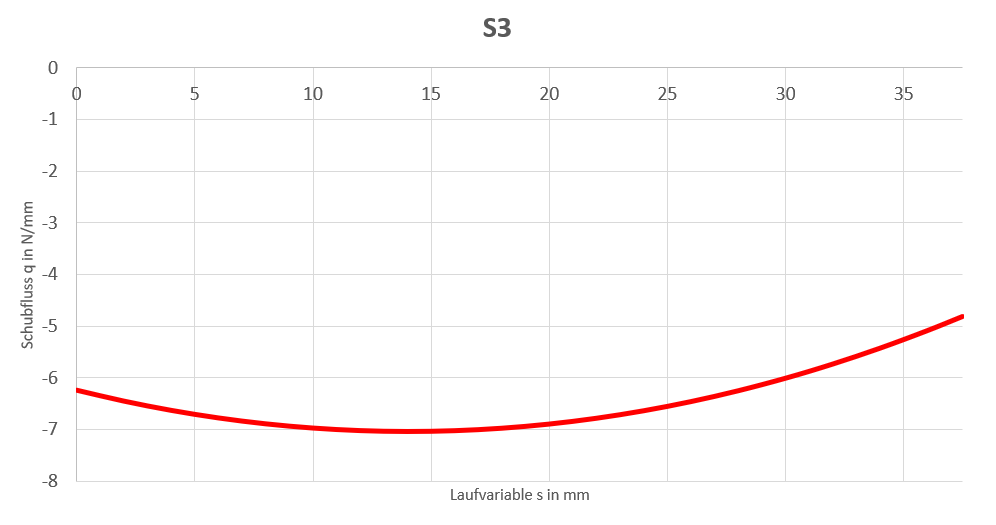
\includegraphics[width=1.0\textwidth]{Bilder/S3.png}
	\caption{Schubfluss Bereich $III$}
	\label{fig:S3}
\end{figure}
\begin{figure}[h]
	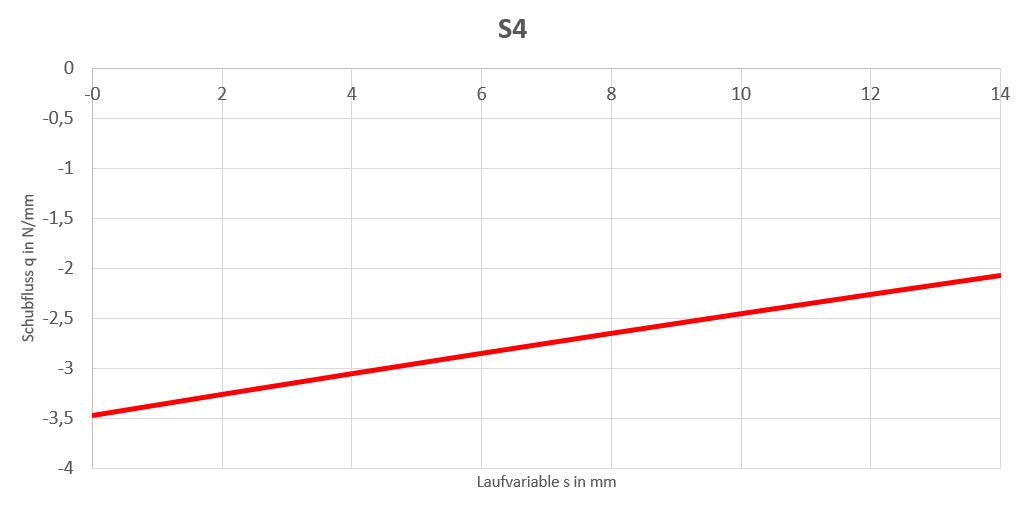
\includegraphics[width=1.0\textwidth]{Bilder/S4.png}
	\caption{Schubfluss Bereich $IV$}
	\label{fig:S4}
\end{figure}
\begin{figure}[h]
	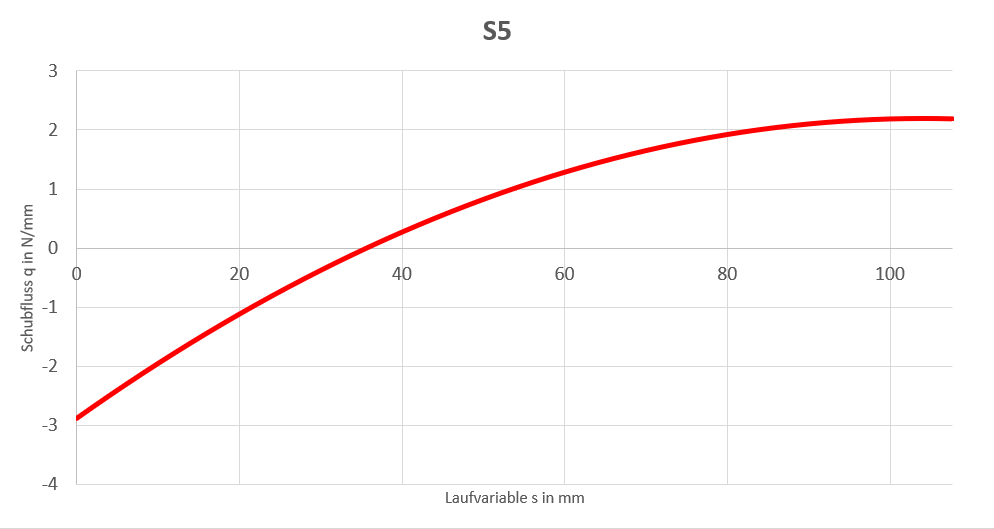
\includegraphics[width=1.0\textwidth]{Bilder/S5.png}
	\caption{Schubfluss Bereich $V$}
	\label{fig:S5}
\end{figure}
\begin{figure}[h]
	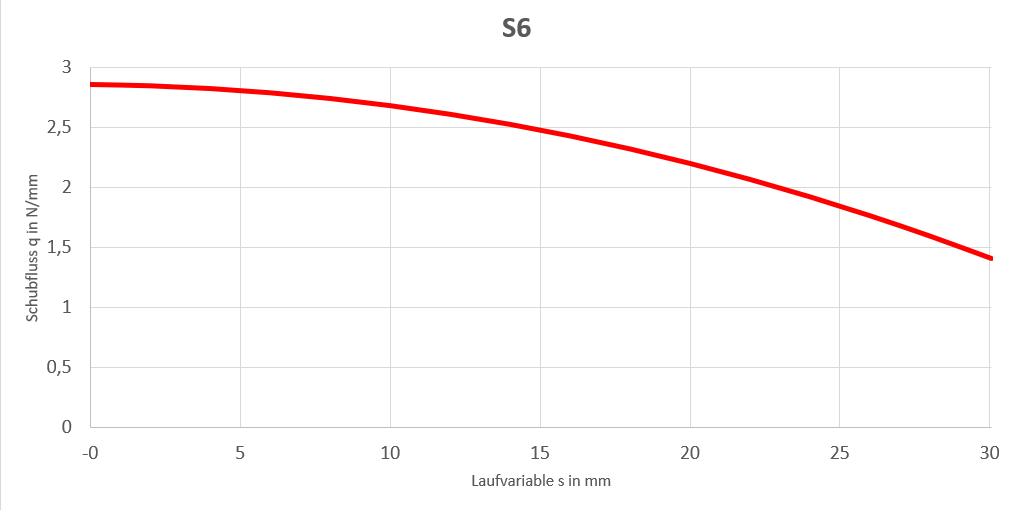
\includegraphics[width=1.0\textwidth]{Bilder/S6.png}
	\caption{Schubfluss Bereich $VI$}
	\label{fig:S6}
\end{figure}
\begin{figure}[h]
	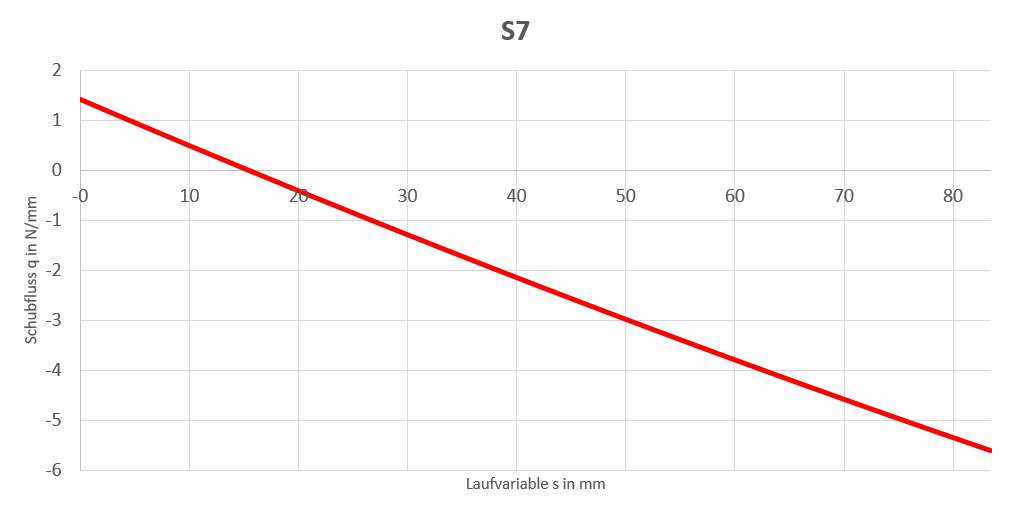
\includegraphics[width=1.0\textwidth]{Bilder/S7.png}
	\caption{Schubfluss Bereich $VII$}
	\label{fig:S7}
\end{figure}
\begin{figure}[h]
	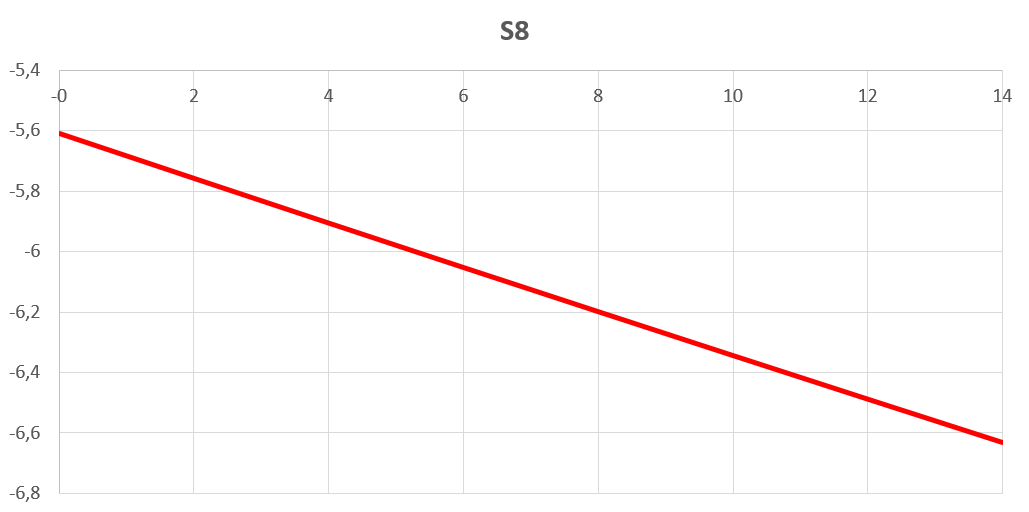
\includegraphics[width=1.0\textwidth]{Bilder/S8.png}
	\caption{Schubfluss Bereich $VIII$}
	\label{fig:S8}
\end{figure}
\begin{figure}[h]
	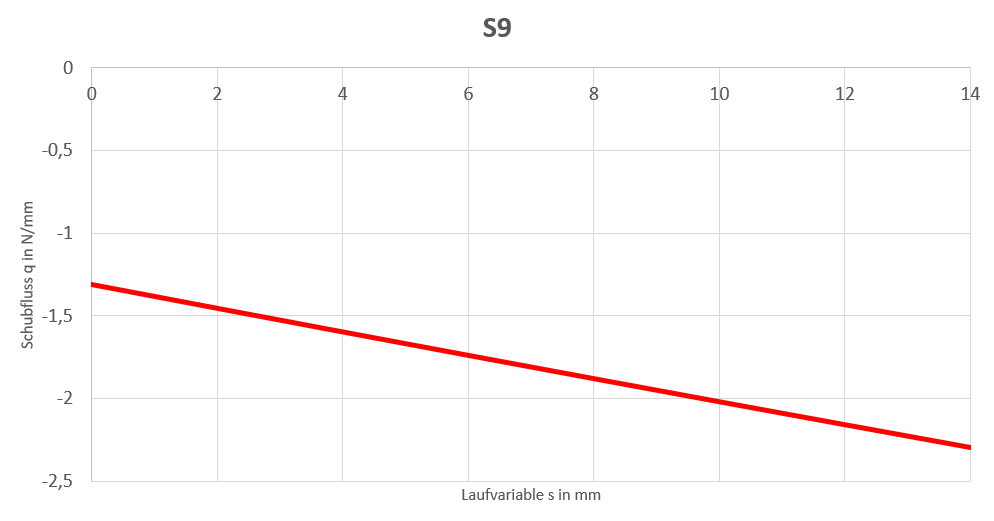
\includegraphics[width=1.0\textwidth]{Bilder/S9.png}
	\caption{Schubfluss Bereich $IX$}
	\label{fig:S9}
\end{figure}
\begin{figure}[h]
	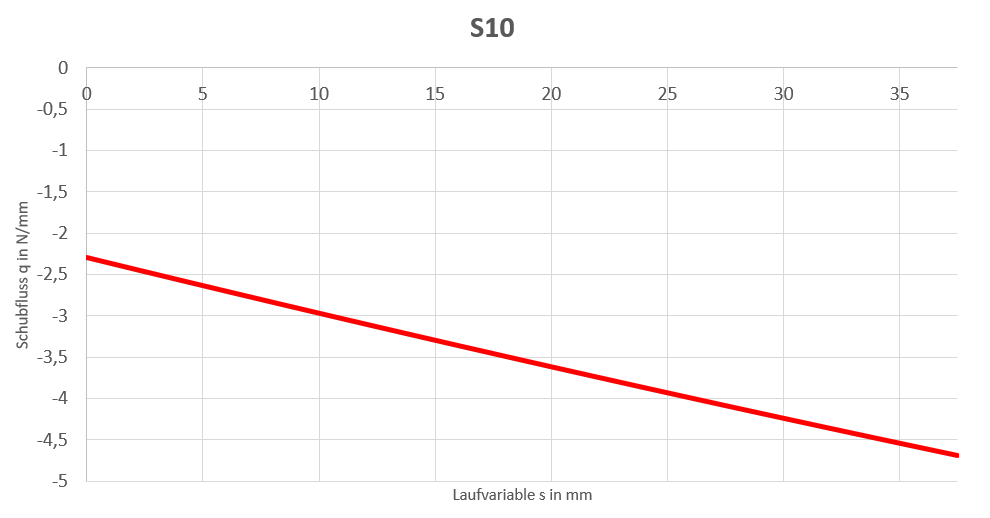
\includegraphics[width=1.0\textwidth]{Bilder/S10.png}
	\caption{Schubfluss Bereich $X$}
	\label{fig:S10}
\end{figure}



\end {document}